\documentclass[12pt]{article}

\usepackage{mathpazo}
\usepackage[T1]{fontenc}
\usepackage{lscape}
\usepackage{floatrow}
\usepackage[natbib=true,style=authoryear,sorting=nyt, uniquelist=false,maxbibnames=9,maxcitenames=2]{biblatex}
\AtEveryBibitem{\clearfield{month}}
\addbibresource{ECA.bib}
%\usepackage[a4paper, total={6in, 8in}]{geometry}
%\linespread{1.5}
\usepackage{rotating}
\usepackage{pifont}
\newcommand{\cmark}{\ding{51}}  % coche
\usepackage{epstopdf}
\usepackage{graphicx}
\usepackage{booktabs}
\usepackage{dcolumn}
\usepackage{caption,subcaption}
\usepackage[dvipsnames]{xcolor}
\definecolor{redfab}{rgb}{0.6, 0.0, 0.0}
\usepackage[colorlinks=true, linkcolor=redfab, citecolor=redfab, urlcolor=black]{hyperref}
\usepackage{etoolbox}
\AtBeginEnvironment{tabular}{\fontsize{10}{12}\selectfont}
\usepackage{siunitx}     % Column number alignment
\usepackage[margin=1in]{geometry} % Page margins
%\usepackage{rotating}
%\counterwithout{figure}{section}
%\setlength{\footnotesep}{10pt}

\providecommand{\sym}[1]{\ifmmode^{#1}\else\(^{#1}\)\fi}

\begin{document}
\title{The Hidden Cost of Globalization in the Underwater World: Evidence from California's Kelp Forests}
\author{\large Fabien Candau\thanks{UPPA E2S, TREE, France. fabien.candau@univ-pau.fr}\thanks{We would like to thank David Nagy, Sandra Poncet, Pamina Koenig, Antoine Bouet, Aicha Hasni, \'{E}lise Labauvie, Isabelle Chort, and Christophe Maes for valuable comments and discussions. We also thank all the participants of several seminars (RITM, BSE, CEEM), particularly Raphael Chiappini, Tanguy Bernard and S\'{e}bastien Desbureaux as well as participants of the 29th Annual Conference of the EAERE.
We are grateful for the excellent working conditions provided by the Atlantic Port of Bordeaux, Bordeaux School of Economics, and Pompeu Fabra University. Finally, we thank the R\'{e}gion Nouvelle-Aquitaine (project PORTeur) for providing all the funds necessary for this research.} \and \large Florian Lafferrere\thanks{UPPA E2S, TREE, France.}}
\maketitle
\begin{abstract}
This article analyzes how maritime regulation affects kelp forests along the California coast. Combining satellite measures of kelp canopy and biomass with AIS vessel trajectories, we exploit variation in pre-policy shipping exposure across kelp cells. After California's Ocean-Going Vessel Fuel Rule (July 2009), kelp improves disproportionately where maritime traffic was highest, with estimated gains of approximately 15--17\% per unit of log shipping exposure. Event studies show no differential pre-trends, with the treatment effect appearing sharply at implementation. We apply the same design to the 2011 boundary modification around the Channel Islands, which re-concentrated vessel traffic in specific corridors. Kelp declined most in the cells that had the highest pre-modification shipping exposure. JEL: Q57, R41, F18

\medskip
\noindent\textbf{Keywords:} Kelp forests, maritime regulation, emission control areas, difference-in-differences, ecosystem services
\end{abstract}

\section{Introduction}

Contemporary globalization relies heavily on maritime routes that generate substantial negative externalities and hidden costs. The consequences of air pollution related to shipping for human health are now well documented (e.g., \citealp{Klotz2022}; \citealp{HansenLewis2022}), but evidence on the impacts on marine ecosystems remains comparatively limited at the spatial scale relevant for policy. A growing body of work shows that environmental regulations can yield ecological co-benefits beyond their primary design targets (\citealp{ShapiroWalker2018}; \citealp{KeiserShapiro2019}). Whether maritime emission controls similarly benefit nearshore ecosystems is an open question. This paper investigates it by quantifying how a major coastal shipping regulation and the associated reconfiguration of traffic patterns relate to the dynamics of kelp forests along the California coast. Our identification strategy isolates a specific physical channel---the spatial footprint of maritime activity---through which international trade affects nearshore ecosystems.

Kelp forests are large biogenic habitats that support coastal biodiversity and provide multiple ecosystem services. As a foundation species (\citealp{Paine1969}; \citealp{Hale2018}), kelp creates habitat structure that functions as nursery grounds and supports complex food webs (\citealp{Christie2009}). Recent global accounting exercises suggest that kelp ecosystems contribute sizable benefits through fisheries production, nutrient cycling, and carbon sequestration (\citealp{Eger2023}; see also \citealp{Costello2020} on the broader economics of marine food systems). Because kelp can respond quickly to changing local conditions through rapid growth and recruitment (\citealp{Krumhansl2016}; \citealp{Carr2019}), it offers an informative setting to study ecosystem responses to changes in nearshore stressors over a relatively short horizon.

We study California's Ocean-Going Vessel Fuel Rule, which established a regulated zone in 2009 and later modified the boundary in southern California in 2011. The policy was designed to reduce sulfur-related emissions by requiring the use of low-sulfur marine distillate fuels within the zone. For our setting, the rule altered vessel routing decisions (\citealp{Klotz2022}), thereby changing the spatial footprint of maritime activity near kelp forests. These routing adjustments provide quasi-experimental variation that can be exploited to learn about the sensitivity of kelp forests to maritime exposure.

Our contribution is twofold. First, we combine quarterly satellite-based measures of kelp canopy and biomass with AIS-derived shipping exposure to implement a continuous difference-in-differences design. We exploit within-zone variation in pre-policy vessel traffic; kelp cells that were more exposed to shipping before 2009 should benefit more if the regulation effectively reduces nearshore pressures. We find evidence consistent with this prediction: the interaction between shipping exposure and the post-policy indicator is positive and significant across all specifications. Event-study estimates show no differential pre-trends in kelp outcomes across exposure levels, strengthening the causal interpretation.

Second, we apply the same continuous difference-in-differences framework to the 2011 boundary modification around the Channel Islands---a change that re-concentrated traffic in specific corridors. Using pre-modification shipping activity as a predetermined treatment intensity, we show that kelp cells more exposed to vessel traffic before 2011 experienced disproportionately worse outcomes after the boundary change. This result mirrors the first finding: cells that benefited most from the 2009 regulation saw kelp recover; cells most affected by the 2011 re-concentration of traffic saw kelp deteriorate. Taken together, the two designs trace out both sides of the same relationship between maritime exposure and kelp health.

This analysis relates to four strands of work. First, it contributes to the economics of trade, environmental regulation, and pollution. Recent work has quantified the environmental costs of CO$_2$ emissions associated with international trade (\citealp{Shapiro2016}), shown that environmental regulation accounts for most of the decline in U.S.\ manufacturing pollution (\citealp{ShapiroWalker2018}), and examined the distributional incidence of carbon pricing (\citealp{GraingerKolstad2010}). Our paper extends this line of work to marine ecological outcomes by providing evidence that trade-related regulation is associated with changes in coastal ecosystem outcomes. Second, it complements research on international economic activity and environmental outcomes by bringing marine forests---kelp in particular---into the economic analysis of deforestation (e.g., \citealp{Berman2023}; \citealp{Abman2020}; \citealp{Carreira2024}; \citealp{Nedoncelle2024}). Third, it complements experimental and site-specific ecological studies on shipping-related stressors (e.g., \citealp{Johansson2012}) by providing a spatially comprehensive, policy-relevant analysis that follows a regulatory change. Fourth, it connects to the literature evaluating emission control policies in maritime settings by documenting ecosystem responses in coastal waters, beyond human-health endpoints (e.g., \citealp{Klotz2022}; \citealp{HansenLewis2022}).\footnote{More broadly, \citet{KeiserShapiro2019} provide a precedent for our approach by estimating the ecological consequences of the Clean Water Act using large-scale environmental monitoring data---a parallel to our use of satellite-based kelp monitoring to evaluate maritime regulation.}

\section{Background}

The California--Baja California coast hosts extensive kelp forests dominated by canopy-forming species (giant kelp, \textit{Macrocystis pyrifera}, and bull kelp, \textit{Nereocystis luetkeana}). These species form surface (or near-surface) canopies that are detectable with satellite imagery (\citealp{Bell2023}). 

Kelp performance is shaped by ocean temperature, nutrient availability, water light (or coastal darkening), as well as localized stressors that can damage fronds, inhibit photosynthesis, or alter community structure (\citealp{Carr2019}). More broadly, climatic variability is a first-order driver of kelp outcomes. Ocean climate oscillations influence sea surface temperatures, salinity, and nutrient availability over multi-year cycles (\citealp{Castorani2022}). Warm-water events can sharply reduce canopy extent, and the decline observed since 2014 has been linked to prolonged warm conditions and cascading ecological interactions (\citealp{RogersBennett2019}; see also \citealp{Krumhansl2016}). These mechanisms motivate the inclusion of sea surface temperature and wave intensity controls in our empirical models.

Maritime activity can affect kelp through several channels. Vessel operations generate discharges (greywater and blackwater) and associated chemical and nutrient loads that can contribute to eutrophication and oxygen depletion (\citealp{Lindgren2016}), with potential consequences for coastal vegetation and algal community composition (e.g., \citealp{FilbeeDexter2018}). Shipping can also introduce contaminants through antifouling practices. Biocidal compounds historically used to reduce hull fouling can enter coastal waters and affect marine organisms (\citealp{Dafforn2011}; \citealp{Cima2022}), with laboratory evidence that antifouling compounds can inhibit kelp photosynthesis and growth (\citealp{Johansson2012}). Finally, maritime traffic can influence nearshore physical conditions (wake, turbulence, localized disturbance) and can concentrate stressors along heavily trafficked corridors.

A distinct, potentially important channel is the introduction of non-native species via hull fouling and ballast water. The literature has documented introductions linked to shipping, with consequences that vary across species and contexts (\citealp{Williams2007}). Evidence on the impacts of particular invaders on native kelp is mixed, including work on \textit{Sargassum muticum} (\citealp{Ambrose1982}; \citealp{BrittonSimmons2004}; \citealp{Smith2015}) and more recent assessments of \textit{Undaria pinnatifida} (\citealp{McHaskell2024}).\footnote{\textit{Undaria pinnatifida} is a kelp from northeast Asia, established in California in the 2000s, and classified as one of the ``100 of the world's worst invasive alien species'' (in the IUCN's list). The invasion of this kelp may have an effect on the native sub-canopy (e.g., on \textit{Pyrifera} and \textit{Pterygophora californica}) but not on the native canopy kelp studied here, which are not found in the same habitats.} Ballast water can also transport grazers and pathogens with ecosystem-wide effects (e.g., \citealp{Phinney2001}). 

While our empirical designs do not identify the relative importance of these channels, they motivate the hypothesis that changes in the spatial distribution and intensity of shipping activity can matter for kelp outcomes. California's Ocean-Going Vessel Fuel Rule introduced a regulated zone extending 24 nautical miles off the coast starting in 2009 that enables us to test this hypothesis. Covered vessels must use low-sulfur marine distillate fuels within the zone. Compliance increases operating costs within the regulated area and can induce changes in routing and the spatial distribution of traffic. As we discuss in Section~\ref{sec:threats}, voyage-level evidence confirms that vessels sharply adjusted routes following implementation (\citealp{Klotz2022}). Finally, in 2011, the southern boundary was modified around the Channel Islands, affecting where ships concentrate as they approach ports and creating additional variation in maritime exposure.

\section{The 2009 Ocean-Going Vessel Fuel Rule}
\label{sec:empirical}

This section describes the data and the continuous difference-in-differences design used to estimate changes in kelp canopy and biomass associated with the 2009 implementation of the regulated zone.

\subsection{Data}\label{sec:data}

We combine satellite kelp observations, AIS vessel tracking data, and environmental covariates, all aggregated to a common spatial grid of 10\,km hexagonal cells at quarterly frequency.

\paragraph{Kelp outcomes and shipping exposure.}
Kelp outcomes come from \citet{Bell2023}, which provides quarterly cloud-free Landsat-based measures of floating kelp canopy at 30m resolution along the Pacific coast.\footnote{The underlying imagery consists of Landsat Collection~1 Level-2 Surface Reflectance products, which apply atmospheric correction for aerosols and water vapor \emph{before} kelp classification. Images with more than 25\% cloud cover are excluded, and remaining cloud and cloud-shadow pixels are masked using the quality-assurance band. Any localized change in atmospheric transparency---such as reduced sulfur aerosols from the fuel regulation---is therefore corrected at the reflectance stage rather than propagated into the kelp canopy estimates.} We use two variables: (i) kelp canopy area within each pixel (m$^{2}$) and (ii) kelp canopy biomass (kg) inferred from validated relationships between surface reflectance and in situ canopy and biomass measurements (\citealp{Bell2023}). Satellite detection captures surface (or near-surface) canopy and does not observe subsurface kelp.

We overlay a uniform grid of 10\,km hexagonal cells covering the study area (the 2009 regulated zone and the 2011 boundary modification area) and aggregate all variables to this common spatial unit at the quarterly frequency.

For each year--quarter, the 30\,m pixel-level kelp observations are converted to point geometries using their latitude and longitude coordinates and spatially joined to the hexagonal grid. Within each hexagon $i$ and quarter $t$, we compute the sum and mean of kelp canopy area (m$^{2}$) and biomass (kg), as well as the count of kelp pixels.

Vessel trajectories are derived from georeferenced ship positions recorded by the Automated Identification System (AIS), made available by the U.S. Coast Guard.\footnote{AIS data accessed via MarineCadastre.gov, jointly maintained by the U.S. BOEM and NOAA.} We focus on four major cargo vessel classes---tankers, container ships, general cargo ships, and bulk carriers---and summarize their activity at the hexagon--month level in terms of total distance traveled within the cell (``length'', in meters) and number of unique vessel passages (``count''). To assign shipping exposure to kelp locations, we proceed as follows. For each hexagon containing kelp, we create a circular buffer of 20\,km radius and identify all shipping hexagons that intersect this buffer. We then aggregate the shipping measures---summing length and count---across all identified shipping hexagons for each kelp hexagon $i$ and quarter $t$. This yields two continuous exposure variables per kelp cell: total distance traveled by vessels in its vicinity ($Length_{it}$) and total number of vessel passages ($Count_{it}$).

Finally, we incorporate the cumulative human impact index of \citet{Halpern2009}, which combines 25 anthropogenic stressors and 19 marine ecosystems to map cumulative pressure on the California Current at ${\sim}$1\,km$^{2}$ resolution (see also \citealp{Maxwell2013}).\footnote{For each pixel the index is $I_{C}=\sum_{s}\sum_{e}D_{s}\,E_{e}\,\mu_{se}$, where $D_{s}$ is the normalized intensity of stressor $s$, $E_{e}$ indicates the presence of ecosystem $e$, and $\mu_{se}$ is an expert-elicited vulnerability weight scored on a 0--4 scale based on spatial extent, frequency, functional impact, resistance, and recovery time.} Using zonal statistics, we compute the mean value of this raster within each 10\,km hexagonal cell, providing a time-invariant measure of baseline anthropogenic pressure at each kelp location.

\paragraph{Environmental controls.}
Kelp forests are affected by multiple interacting environmental drivers, including temperature, water motion, and nutrient availability (\citealp{Carr2019}; \citealp{Castorani2022}). We include three time-varying physical controls that are well-established determinants of kelp dynamics.

Sea surface temperature (SST) is sourced from MODIS monthly composites and aggregated to quarters. SST is a central determinant of kelp dynamics and is also informative about broader ocean conditions (e.g., \citealp{Yang2023}; \citealp{Dunstan2018}).\footnote{We do not include a separate upwelling index (e.g., CUTI or BEUTI; \citealp{Jacox2018}) because SST is strongly negatively correlated with upwelling intensity along the California coast---cold surface water is the primary physical signature of upwelling events---and our year--quarter fixed effects already absorb the dominant seasonal upwelling cycle. Any remaining bias would require a differential change in upwelling at the policy date that is spatially correlated with shipping exposure.} Wave intensity is drawn from ERA5 (\citealp{Hersbach2023}) and measured as significant wave height (the average height of the highest third of waves), aggregated to quarters; it captures physical stress associated with storms and strong sea states. Precipitation is drawn from ERA5 and aggregated to quarters; it proxies terrestrial nutrient runoff, which can affect kelp growth.

\subsection{Specification}

Our main design is a continuous difference-in-differences (\citealp{CallawayGoodmanBaconSantAnna2024}) that exploits cross-sectional variation in pre-policy shipping exposure. The intuition is straightforward: kelp cells that were more exposed to vessel traffic before 2009 should benefit more from the implementation of the regulated zone if that regulation effectively reduces nearshore stressors. The treatment intensity is measured by pre-policy shipping activity derived from AIS data: logged mean vessel traffic (measured as total distance traveled) or logged mean vessel count within a 20\,km buffer around each kelp hexagon during January--June 2009, before implementation.

We estimate:
\begin{equation}
Kelp_{it}=\exp\!\left(\beta\,Exposure_{i}\times \mathit{Post2009}_{t}+\delta\,Z_{it}+f_{i}+f_{t}\right)\cdot\eta_{it},
\label{eq:cdid}
\end{equation}
where $\eta_{it}$ is a multiplicative error term satisfying $E[\eta_{it}\mid Exposure_{i},Z_{it},f_{i},f_{t}]=1$, and $Kelp_{it}$ is the sum of kelp biomass (kg) or canopy area (m$^{2}$) in hexagonal cell $i$ during quarter $t$. $Exposure_{i}$ is the time-invariant, predetermined measure of shipping activity described above (logged mean vessel traffic or logged mean vessel count, January--June 2009). $\mathit{Post2009}_{t}$ equals one from 2009Q3 onward and zero otherwise. $Z_{it}$ is a vector of log-transformed environmental controls (log sea surface temperature, log precipitation, and log significant wave height).\footnote{All controls are transformed as $\ln(1+x)$. For SST and significant wave height, which are strictly positive and large in magnitude, this is virtually identical to $\ln(x)$. For precipitation, the $\ln(1+x)$ form handles quarters with zero rainfall.} $f_{i}$ denotes kelp-cell fixed effects (one indicator per hexagonal cell) and $f_{t}$ denotes year--quarter fixed effects. The cell fixed effects absorb any time-invariant determinant of kelp outcomes---including the main effect of $Exposure_{i}$---and the time fixed effects absorb shocks common to all cells, including the main effect of $\mathit{Post2009}_{t}$.

Because kelp outcomes are non-negative and include many zeros, we estimate Eq.~(\ref{eq:cdid}) by Poisson pseudo-maximum likelihood (PPML; \citealp{SantosSilva2006}).\footnote{We restrict the sample to cells recording at least two vessel passages per month on average during January--June 2009, excluding cells with negligible shipping exposure. Results are robust to alternative cutoffs (Figure~\ref{fig:weighting_diagnostic}) and to weighting by log vessel count (\hyperref[appendix_weighted]{Appendix~\ref*{appendix_weighted}}).} Standard errors are clustered at the cell level (81 clusters).\footnote{Because kelp cells are hexagons along a narrow coastal strip, adjacent cells may share ocean currents and temperature fields, inducing spatial correlation within clusters. Conley standard errors \citep{Conley1999} which allow for spatial dependence decaying with distance, are the natural remedy in OLS settings but are not available for PPML: the Conley estimator relies on a sandwich formula for the linear GMM moment conditions, which does not directly extend to the nonlinear PPML first-order conditions. Implementing spatial HAC inference for Poisson models would require either a nonlinear GMM framework or a spatial bootstrap, neither of which is standard in the literature. We note this as a limitation and a direction for future methodological work.} The sample covers Southern California (latitudes 32\textdegree--36\textdegree N) from 2005 to 2016. The year--quarter fixed effects absorb any coast-wide ecological shock, including the 2013--2016 marine heat wave that caused catastrophic kelp losses in northern California (\citealp{RogersBennett2019}; \citealp{McPherson2021}). Such a shock would bias $\beta$ only if its spatial footprint were systematically correlated with the pre-policy shipping-exposure cross-section, for which there is no ecological basis.

The coefficient of interest is $\beta$. A positive $\beta$ indicates that, after implementation, kelp outcomes improved disproportionately in cells that were more exposed to vessel traffic before the policy---consistent with the regulation improving conditions in areas where maritime activity was most concentrated.

This continuous design offers two advantages over a binary treated-versus-control comparison. First, it does not require selecting a specific control group outside the regulated zone; identification comes from variation in pre-policy exposure \emph{within} the regulated area. Second, using a continuous treatment intensity exploits the full cross-sectional variation in exposure rather than collapsing it into a binary indicator, yielding a more powerful test of whether kelp forests that were more exposed to maritime traffic recover disproportionately after the implementation of the ECA.

As a complementary exercise, \hyperref[appendix_weighted]{Appendix~\ref*{appendix_weighted}} reports a specification replacing our AIS-based exposure with the cumulative human impact index of \citet{Halpern2009} described in Section~\ref{sec:data}. Although the coefficient is also positive and significant, event-study diagnostics reveal pre-existing differential trends driven by non-shipping stressors bundled in the index (urbanization, fishing pressure, nutrient runoff). This motivates our preference for shipping-specific measures, which isolate the regulatory channel.

\subsection{Results}

Table~\ref{tab:main_2009} reports estimates of the continuous difference-in-differences using pre-policy shipping exposure as treatment intensity. Columns~(1)--(2) measure exposure by total distance traveled by vessels (``Distance Traveled (km)''), with biomass and canopy area as dependent variables respectively. Columns~(3)--(4) measure exposure by the number of vessel passages (``Vessel Count'').

\begin{table}[H]
  \centering
  \caption{Continuous difference-in-differences: Kelp outcomes and the 2009 ECA}
  \label{tab:main_2009}
  \def\sym#1{\ifmmode^{#1}\else\(^{#1}\)\fi}
\begin{tabular}{l*{4}{c}}
\hline\hline
                    &\multicolumn{2}{c}{Distance Traveled}&\multicolumn{2}{c}{Vessel Count}\\
                    \cmidrule(lr){2-3}\cmidrule(lr){4-5}
                    &\multicolumn{1}{c}{(1)}&\multicolumn{1}{c}{(2)}&\multicolumn{1}{c}{(3)}&\multicolumn{1}{c}{(4)}\\
                    &\multicolumn{1}{c}{Biomass}&\multicolumn{1}{c}{Area}&\multicolumn{1}{c}{Biomass}&\multicolumn{1}{c}{Area}\\
\hline
Post 2009 $\times$ Exposure&     0.1361\sym{***}&     0.1317\sym{***}&     0.1548\sym{***}&     0.1493\sym{***}\\
                    &             (0.0359)&             (0.0352)&             (0.0432)&             (0.0424)\\
[1em]
SST                 &     -5.703\sym{***}&     -5.512\sym{***}&     -5.728\sym{***}&     -5.537\sym{***}\\
                    &              (1.145)&              (1.136)&              (1.150)&              (1.142)\\
[1em]
Precipitation       &     0.0764&     0.0812&     0.0846&     0.0891\\
                    &             (0.1003)&             (0.0981)&             (0.1012)&             (0.0989)\\
[1em]
Significant Wave Height&     -3.267\sym{**}&     -3.102\sym{**}&     -3.358\sym{**}&     -3.189\sym{**}\\
                    &              (1.367)&              (1.344)&              (1.367)&              (1.342)\\
[1em]
\hline
Cell FE             &         Yes         &         Yes         &         Yes         &         Yes         \\
Year-Quarter FE     &         Yes         &         Yes         &         Yes         &         Yes         \\
Observations        &        3880         &        3880         &        3880         &        3880         \\
\hline\hline
\end{tabular}
  \vspace{0.5em}

  \begin{minipage}{\linewidth}
  \footnotesize
  \textit{Notes:} Unweighted PPML estimates of Eq.~(\ref{eq:cdid}). The dependent variable is kelp biomass (kg) or canopy area (m$^{2}$). ``Distance Traveled (km)'' columns~(1)--(2) measure exposure by logged mean distance traveled by vessels within a 20\,km buffer around each kelp hexagon during January--June 2009; ``Vessel Count'' columns~(3)--(4) use the corresponding logged mean vessel count. All specifications include kelp-cell and year--quarter fixed effects. Sample: Southern California (32\textdegree--36\textdegree\,N), 2005--2016, restricted to cells with at least two vessel passages per month on average (81 cells $\times$ 48 quarters, less 8 cell-quarters with missing covariates in 2015--2016 = 3,880 observations). Standard errors clustered at the cell level (81 clusters) in parentheses. Weighted estimates are reported in \hyperref[appendix_weighted]{Appendix~\ref*{appendix_weighted}}.\\
  \sym{*} \(p<0.10\), \sym{**} \(p<0.05\), \sym{***} \(p<0.01\).
  \end{minipage}
\end{table}

Across all specifications, the interaction between post-2009 implementation and pre-policy shipping exposure is positive and statistically significant at the 1\% level. The estimates are stable across treatment-intensity measures and dependent variables.

In columns~(1)--(2), which use distance traveled by vessels, the coefficient of approximately 0.136 implies that a one-unit increase in log pre-policy distance traveled is associated with an $\exp(0.136)-1\approx 14.6\%$ larger post-2009 increase in expected kelp biomass and canopy. In columns~(3)--(4), the coefficient on vessel count is approximately 0.155, implying a roughly $16.7\%$ relative increase per unit of log vessel count. This consistency across the two shipping measures is reassuring, as they capture different dimensions of maritime activity (total distance traveled versus number of passages).

Environmental controls enter with expected signs. Sea surface temperature is strongly and negatively associated with kelp outcomes across all columns, consistent with the well-documented sensitivity of kelp to warm-water conditions (\citealp{Carr2019}; \citealp{RogersBennett2019}). Significant wave height is also negatively associated with kelp, consistent with physical damage to fronds and holdfasts during strong sea states. Precipitation is positively associated with kelp, possibly reflecting increased terrestrial nutrient runoff that can support kelp growth under moderate conditions.

\subsection{Dynamic effects}
\label{sec:dynamic}

To assess whether the parallel-trends assumption holds and to trace the evolution of treatment effects over time, we estimate an event-study specification:
\begin{equation}
Kelp_{it}=\exp\!\left(\sum_{\ell\neq 2008}\beta_{\ell}\,Exposure_{i}\times\mathbf{1}_{t\in\ell}+\delta\,Z_{it}+f_{i}+f_{t}\right)\cdot\eta_{it},
\label{eq:es}
\end{equation}
where $\ell$ indexes event-study periods and $\mathbf{1}_{t\in\ell}$ equals one when quarter $t$ falls in period $\ell$. Each calendar year constitutes a single period, except 2009, which is split into H1 (Q1--Q2, pre-enforcement) and H2 (Q3--Q4, post-enforcement). The reference period is 2008. This specification interacts the time-invariant treatment intensity with period indicators, allowing us to trace out the differential evolution of kelp outcomes across cells with different levels of shipping exposure.

Figure~\ref{fig:event_study_main} reports the estimated coefficients $\hat{\beta}_{\ell}$ for distance traveled interacted with period indicators, estimated by PPML with the same controls and fixed effects as Eq.~(\ref{eq:cdid}).

\begin{figure}[H]
    \centering
    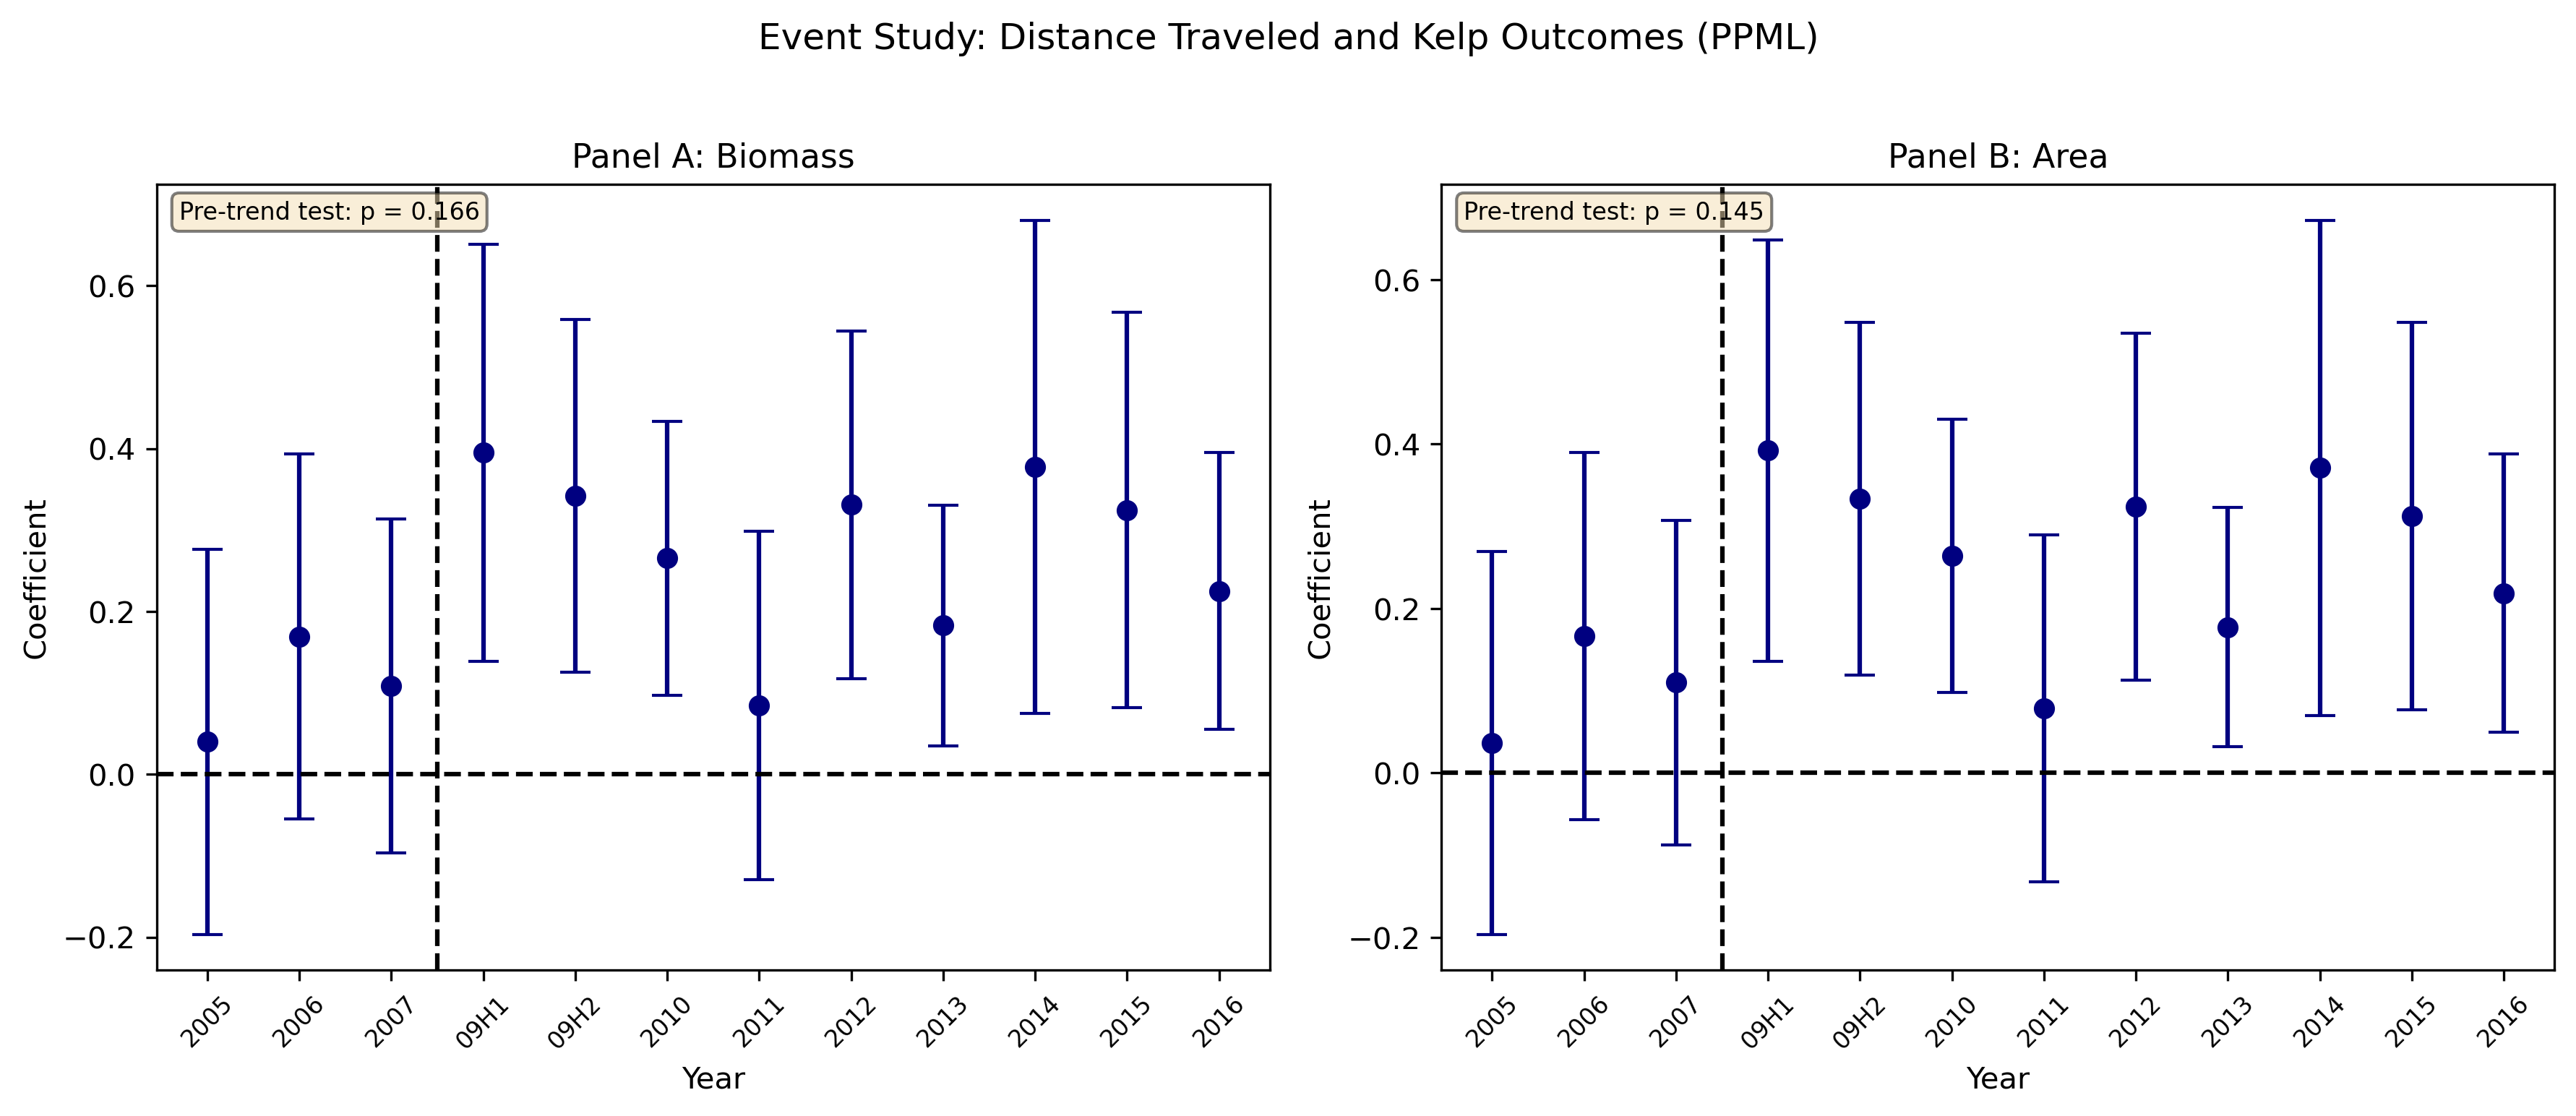
\includegraphics[width=0.95\textwidth]{../output/figures/event_study_main.png}
    \caption{Event study: Distance traveled and kelp outcomes (PPML)}
    \label{fig:event_study_main}
    \vspace{0.15em}
    \begin{flushleft}
        \footnotesize Note: Each panel plots the coefficients from Eq.~(\ref{eq:es}), where distance traveled (logged mean, January--June 2009) is interacted with year indicators, estimated by PPML. The reference year is 2008. The vertical dashed line marks the start of enforcement (2009Q3). Error bars are 95\% confidence intervals based on standard errors clustered at the cell level. Panel~A: kelp biomass; Panel~B: kelp canopy area.
    \end{flushleft}
\end{figure}

Two features of Figure~\ref{fig:event_study_main} merit attention. First, all pre-policy coefficients (2005, 2006, and 2007) are close to zero and statistically insignificant, and a joint Wald test fails to reject the null of no pre-trend ($p=0.17$ for biomass, $p=0.15$ for area), though the power of this test is limited with only three pre-treatment periods. Second, the coefficients turn positive and significant starting in 2009H1---the six months immediately before enforcement---and remain so through the end of the sample (2016), with a temporary dip in 2011. The fact that the effect emerges already in 2009H1 is consistent with some operators switching to compliant fuel during the compliance ramp-up period preceding the July 2009 enforcement date, though mild anticipation or a coincident shock cannot be fully ruled out. The coefficients are similar in magnitude in 2009H1 and 2009H2, suggesting a relatively smooth onset rather than a discrete jump at enforcement. A placebo test setting the treatment date at 2007Q3 on the pre-policy sample alone confirms no effect ($p\geq 0.26$; \hyperref[appendix_placebo]{Appendix~\ref*{appendix_placebo}}). The next subsection examines what these patterns imply for identification.

\subsection{Threats to identification}
\label{sec:threats}

The identifying assumption behind Eq.~(\ref{eq:cdid}) is that, absent the policy, kelp cells with different levels of pre-policy shipping exposure would have followed parallel trajectories. We now assess this assumption in light of the results.

\paragraph{Pre-trends.} As documented above, the event study (Figure~\ref{fig:event_study_main}) shows no systematic differential pre-trend (joint Wald test $p=0.17$; see also \citealp{RambachanRoth2023} on the interpretation of pre-trend tests). \hyperref[appendix_balance]{Appendix~\ref*{appendix_balance}} reports a balance table showing that pre-treatment environmental covariates (SST, precipitation) are comparable across treatment-intensity quartiles, while kelp outcomes and wave height differ---consistent with the geographic concentration of shipping near specific coastal segments. A placebo test using a fake treatment date reinforces this conclusion (\hyperref[appendix_placebo]{Appendix~\ref*{appendix_placebo}}).

\paragraph{Traffic response to the policy.} Our identification strategy treats shipping exposure as a predetermined intensity measure and tests whether kelp outcomes improve differentially in more-exposed cells after the policy date. A natural question is whether the policy actually altered vessel behavior. \citet{Klotz2022} provide direct, voyage-level evidence. Using one-minute AIS data for roughly 20,000 voyages per year off the U.S.\ west coast, they document a sharp discontinuity at the July 2009 enforcement date: container ships reduced fuel consumption within the ECA by 33--52\%, primarily by rerouting outside the regulated boundary---exiting the zone as quickly as possible and traveling south of the Channel Islands rather than through the Santa Barbara Channel. Speed reductions within the ECA reinforced the effect. The 2011 boundary modification around the Channel Islands partially reversed the avoidance pattern, drawing some traffic back into the channel. These voyage-level behavioral shifts are precisely the variation in shipping intensity that our cell-level treatment variable captures, and they confirm that the policy generated a meaningful change in nearshore maritime activity at both dates exploited in our analysis.

\paragraph{Financial crisis.} The most salient contemporaneous shock is the 2008--09 global financial crisis, which reduced trade volumes and port throughput at Southern California ports by roughly 20\% in 2009. If reduced port-related economic activity differentially improved conditions in high-shipping cells through channels unrelated to the ECA (e.g., reduced industrial discharge or ancillary vessel traffic), it could confound our estimates. \hyperref[appendix_crisis]{Appendix~\ref*{appendix_crisis}} addresses this concern directly by constructing a cell-level measure of port economic activity from the National Ballast Information Clearinghouse (NBIC) vessel arrival database and adding it as a time-varying control. The shipping-exposure coefficient is virtually unchanged (at most 2\% attenuation). This coefficient stability when controlling for port activity is the most direct evidence that the crisis does not confound the ECA effect.

\paragraph{Anticipation.} Because CARB adopted the regulation in 2008, vessel operators may have begun rerouting before the July 2009 enforcement date, potentially contaminating our January--June 2009 treatment measure. There are strong economic reasons to discount this concern. The regulation requires the use of low-sulfur marine fuel within the ECA, which is substantially more expensive than the heavy fuel oil used outside it \citep{Klotz2022}. Switching to compliant fuel before enforcement was required would raise operating costs with no offsetting benefit, since penalties for noncompliance did not apply until July 2009. Vessel operators therefore had a clear incentive to maintain pre-policy routing patterns until the enforcement date. The event study is broadly consistent with this reasoning: the 2009H1 coefficient is positive and statistically significant, but similar in magnitude to 2009H2, suggesting a smooth onset of the effect during the compliance ramp-up period rather than anticipatory rerouting. This pattern is compatible with some operators beginning to use low-sulfur fuel in the months before mandatory enforcement, as documented in comparable regulatory settings. The pre-policy coefficients (2005--2007) remain close to zero---the break occurs precisely at the transition to the enforcement year, not gradually over the pre-period. \hyperref[appendix_anticipation]{Appendix~\ref*{appendix_anticipation}} provides further evidence, showing that the cross-sectional ranking of cells by shipping intensity is highly stable in years unaffected by the 2011 boundary modification (Spearman $\rho \geq 0.94$ for 2009, 2012--2014), with a temporary dip in 2010--2011 ($\rho$ between 0.63 and 0.76) driven by the traffic reshuffling around the Channel Islands. Replacing the baseline treatment with 2012 AIS data yields similar coefficients. These patterns confirm that the treatment variable captures stable geographic variation in shipping intensity rather than transient noise.

\paragraph{Spillovers.} If the policy redistributed vessel traffic from high-exposure to low-exposure cells, kelp improvements in treated cells could partly reflect worsened conditions in nearby untreated cells, violating SUTVA. Two features of our design mitigate this concern. First, the 10\,km hexagonal aggregation internalizes local physical spillovers (e.g., pollution or turbidity drifting between adjacent pixels) within each unit. Second, for the broader rerouting-induced interference---where traffic displaced from one corridor reappears in another---the complementary exercise described next, which uses an external control group, is immune to this concern by construction.

\paragraph{External validation.} We subject the main findings to a complementary exercise that relies on an entirely different identification strategy. Following \citet{Arkhangelsky2021}, we construct a synthetic counterpart for treated California hexagons using a donor pool of Mexican coastal hexagons. The estimated post-2009 effect is positive and significant, and the result holds whether we include or exclude southern California hexagons from the treated sample. Full details---sample construction, donor weights, and the synthetic-versus-treated trajectory---are reported in \hyperref[appendix_sc]{Appendix~\ref*{appendix_sc}}. Because the continuous DiD and the synthetic DiD differ in spatial unit, control group, and identifying variation, their convergence strengthens confidence that the pattern reflects a genuine policy effect rather than an artifact of a single design choice.

\section{Boundary Modification of the Regulated Zone in 2011}
\label{sec:extension2011}

This section exploits the 2011 boundary modification around the Channel Islands to provide a second, mirror-image test of the relationship between maritime exposure and kelp health. While Section~\ref{sec:empirical} showed that kelp improved after 2009 in cells more exposed to pre-policy vessel traffic, the 2011 episode allows us to test the converse: whether kelp \emph{deteriorated} in cells more exposed to shipping when the boundary change re-concentrated traffic in specific corridors. Applying the same continuous difference-in-differences logic to a policy change that \emph{increased} rather than decreased local maritime pressure provides a partially independent test that strengthens the causal interpretation of both results.

\subsection{Spatial redistribution of traffic after 2011}

This section relies on the same AIS-derived shipping measures (vessel count and distance traveled) described in Section~\ref{sec:empirical} and assigned to kelp hexagons via the buffer procedure defined above.

The 2011 boundary modification around the Channel Islands altered where vessels concentrate as they approach Southern California ports and contributed to a reallocation of traffic toward specific corridors (\citealp{Klotz2022}). Figures~\ref{fig:shipping_exposure_2009} and~\ref{fig:shipping_exposure_2011} illustrate the baseline spatial distribution of traffic exposure in 2009 and 2011, respectively; \hyperref[appendix_after_2011]{Appendix~\ref*{appendix_after_2011}} documents the post-modification redistribution directly.

\begin{figure}[H]
    \centering
    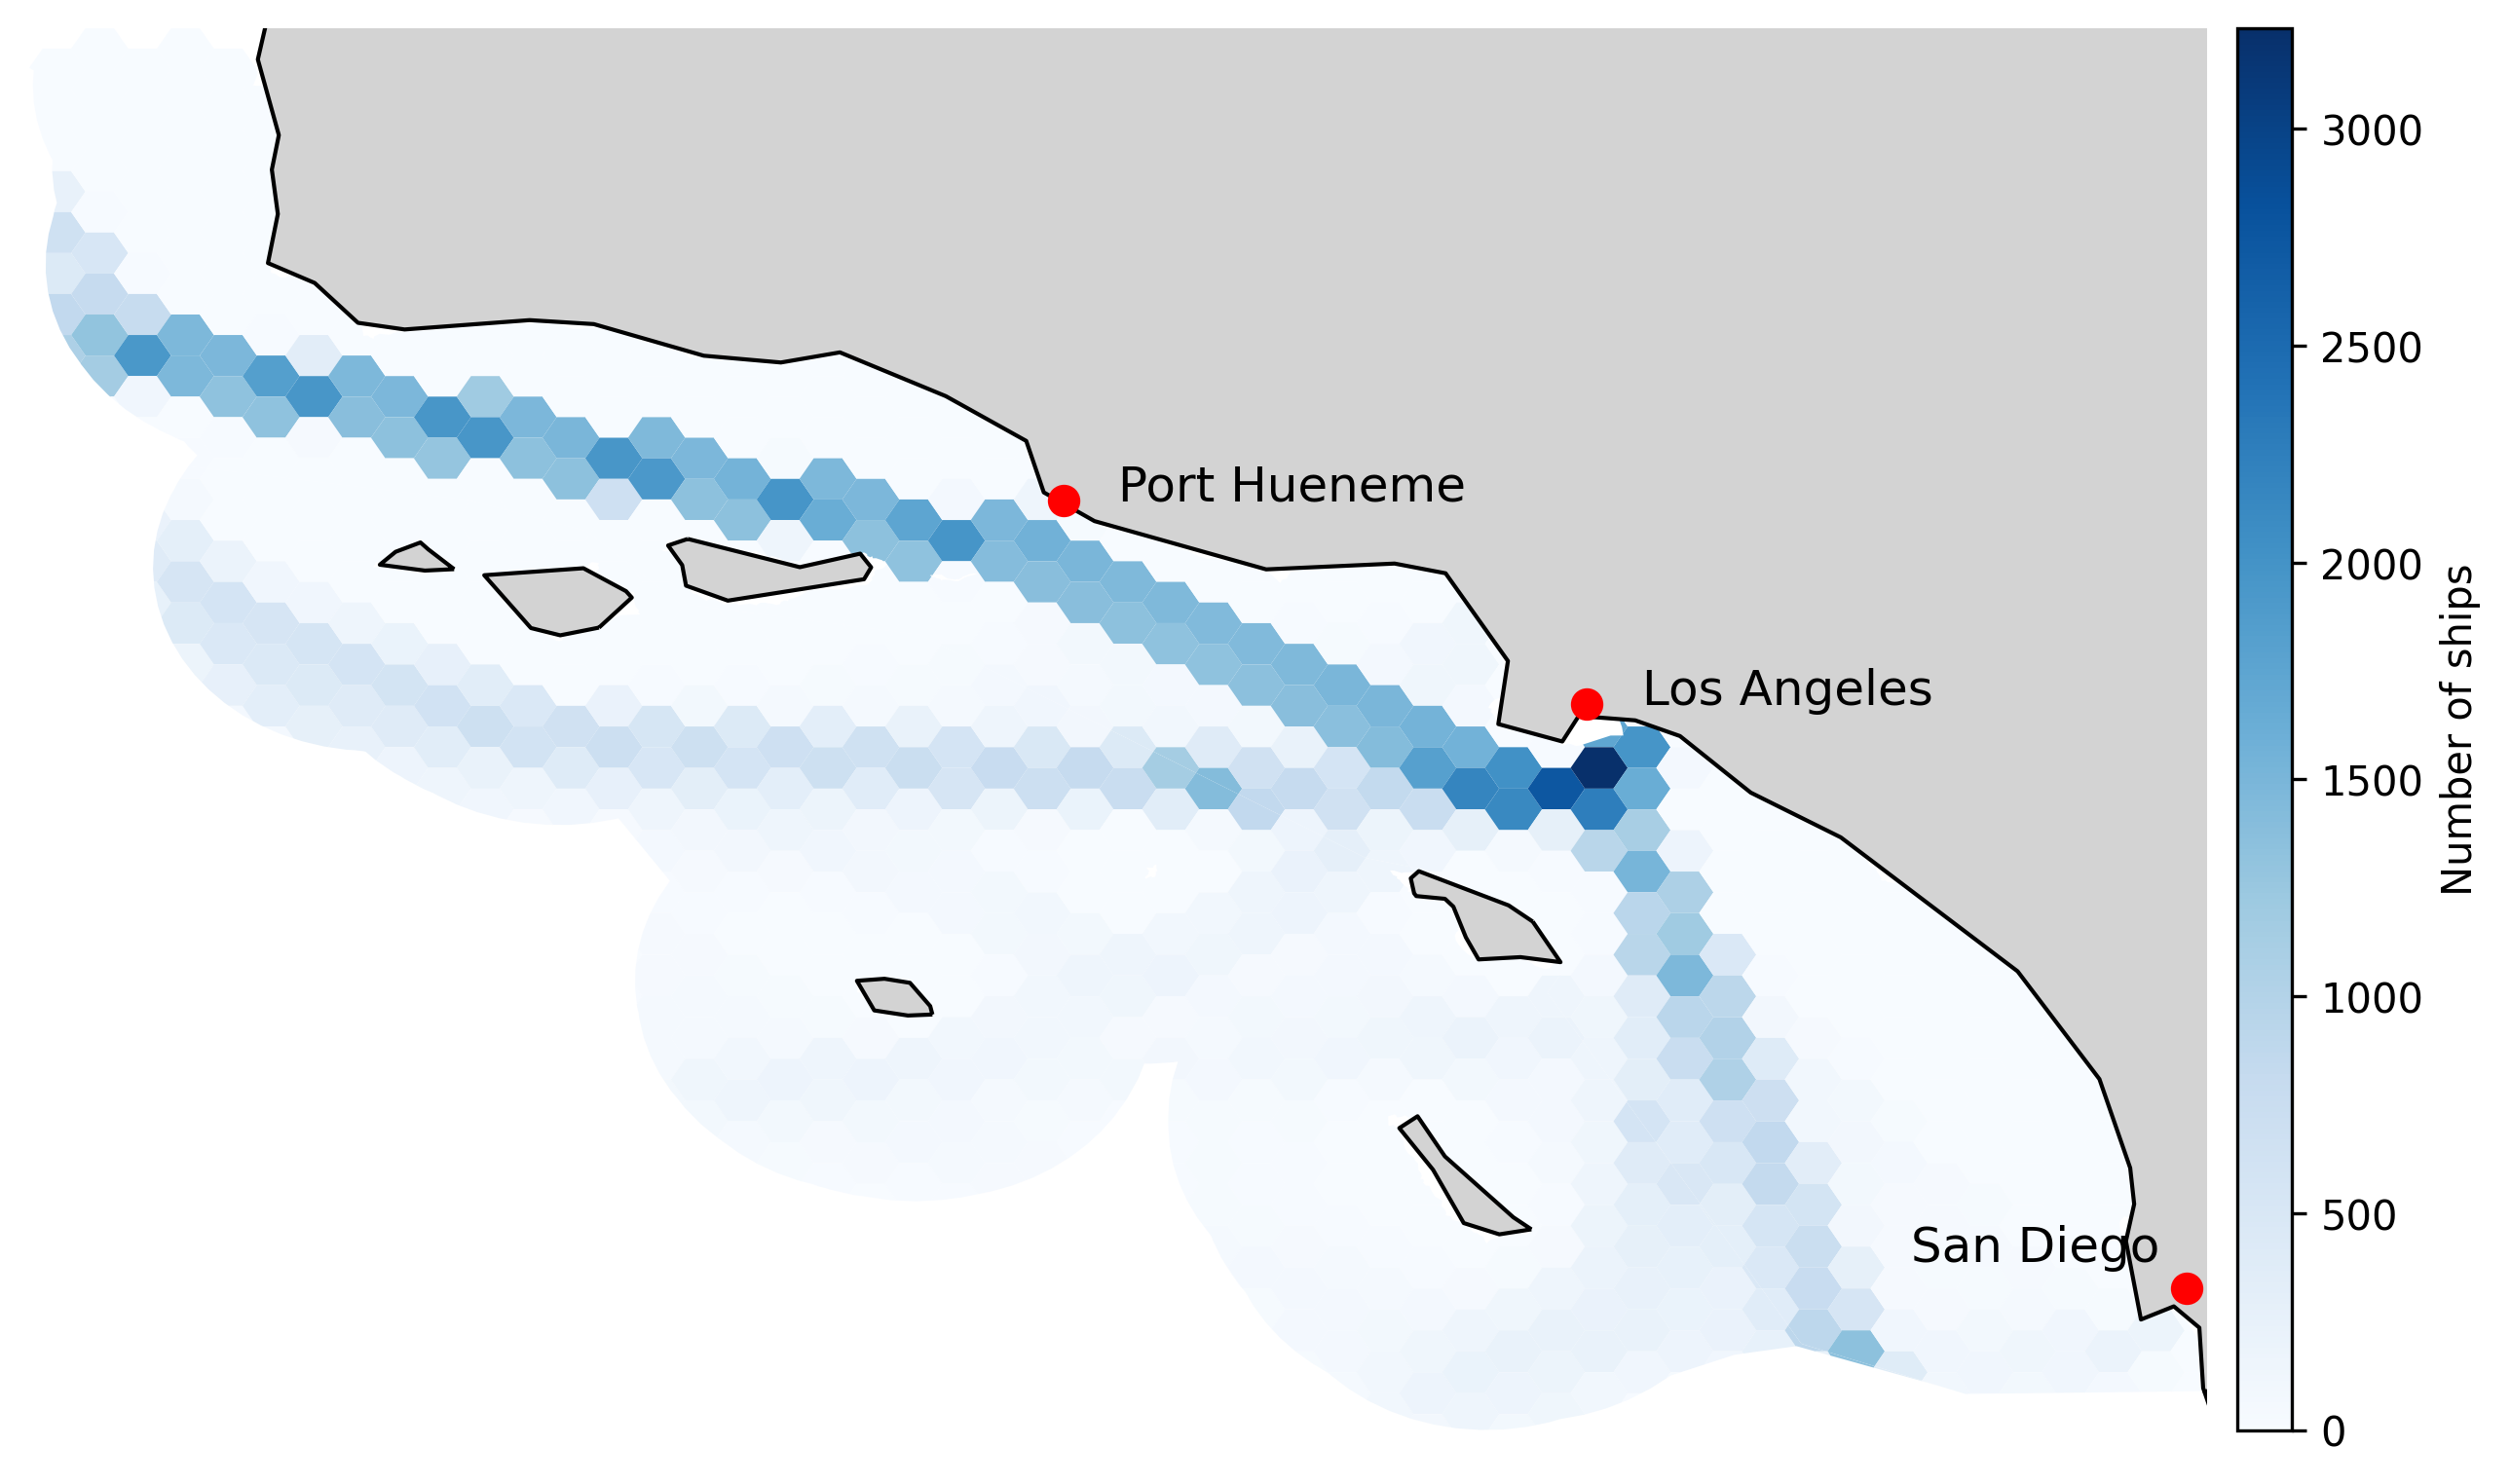
\includegraphics[width=0.7\textwidth]{../output/figures/shipping_exposure_2009.png}
    \caption{Exposure of kelp to maritime traffic in 2009}
    \label{fig:shipping_exposure_2009}
    \vspace{0.5em}
    \begin{flushleft}
{\footnotesize \textit{Notes:} Number of vessel passages through each 10\,km hexagonal cell in Southern California during 2009. Darker shading indicates higher traffic intensity. Data source: AIS.}
    \end{flushleft}
\end{figure}

\begin{figure}[H]
    \centering
    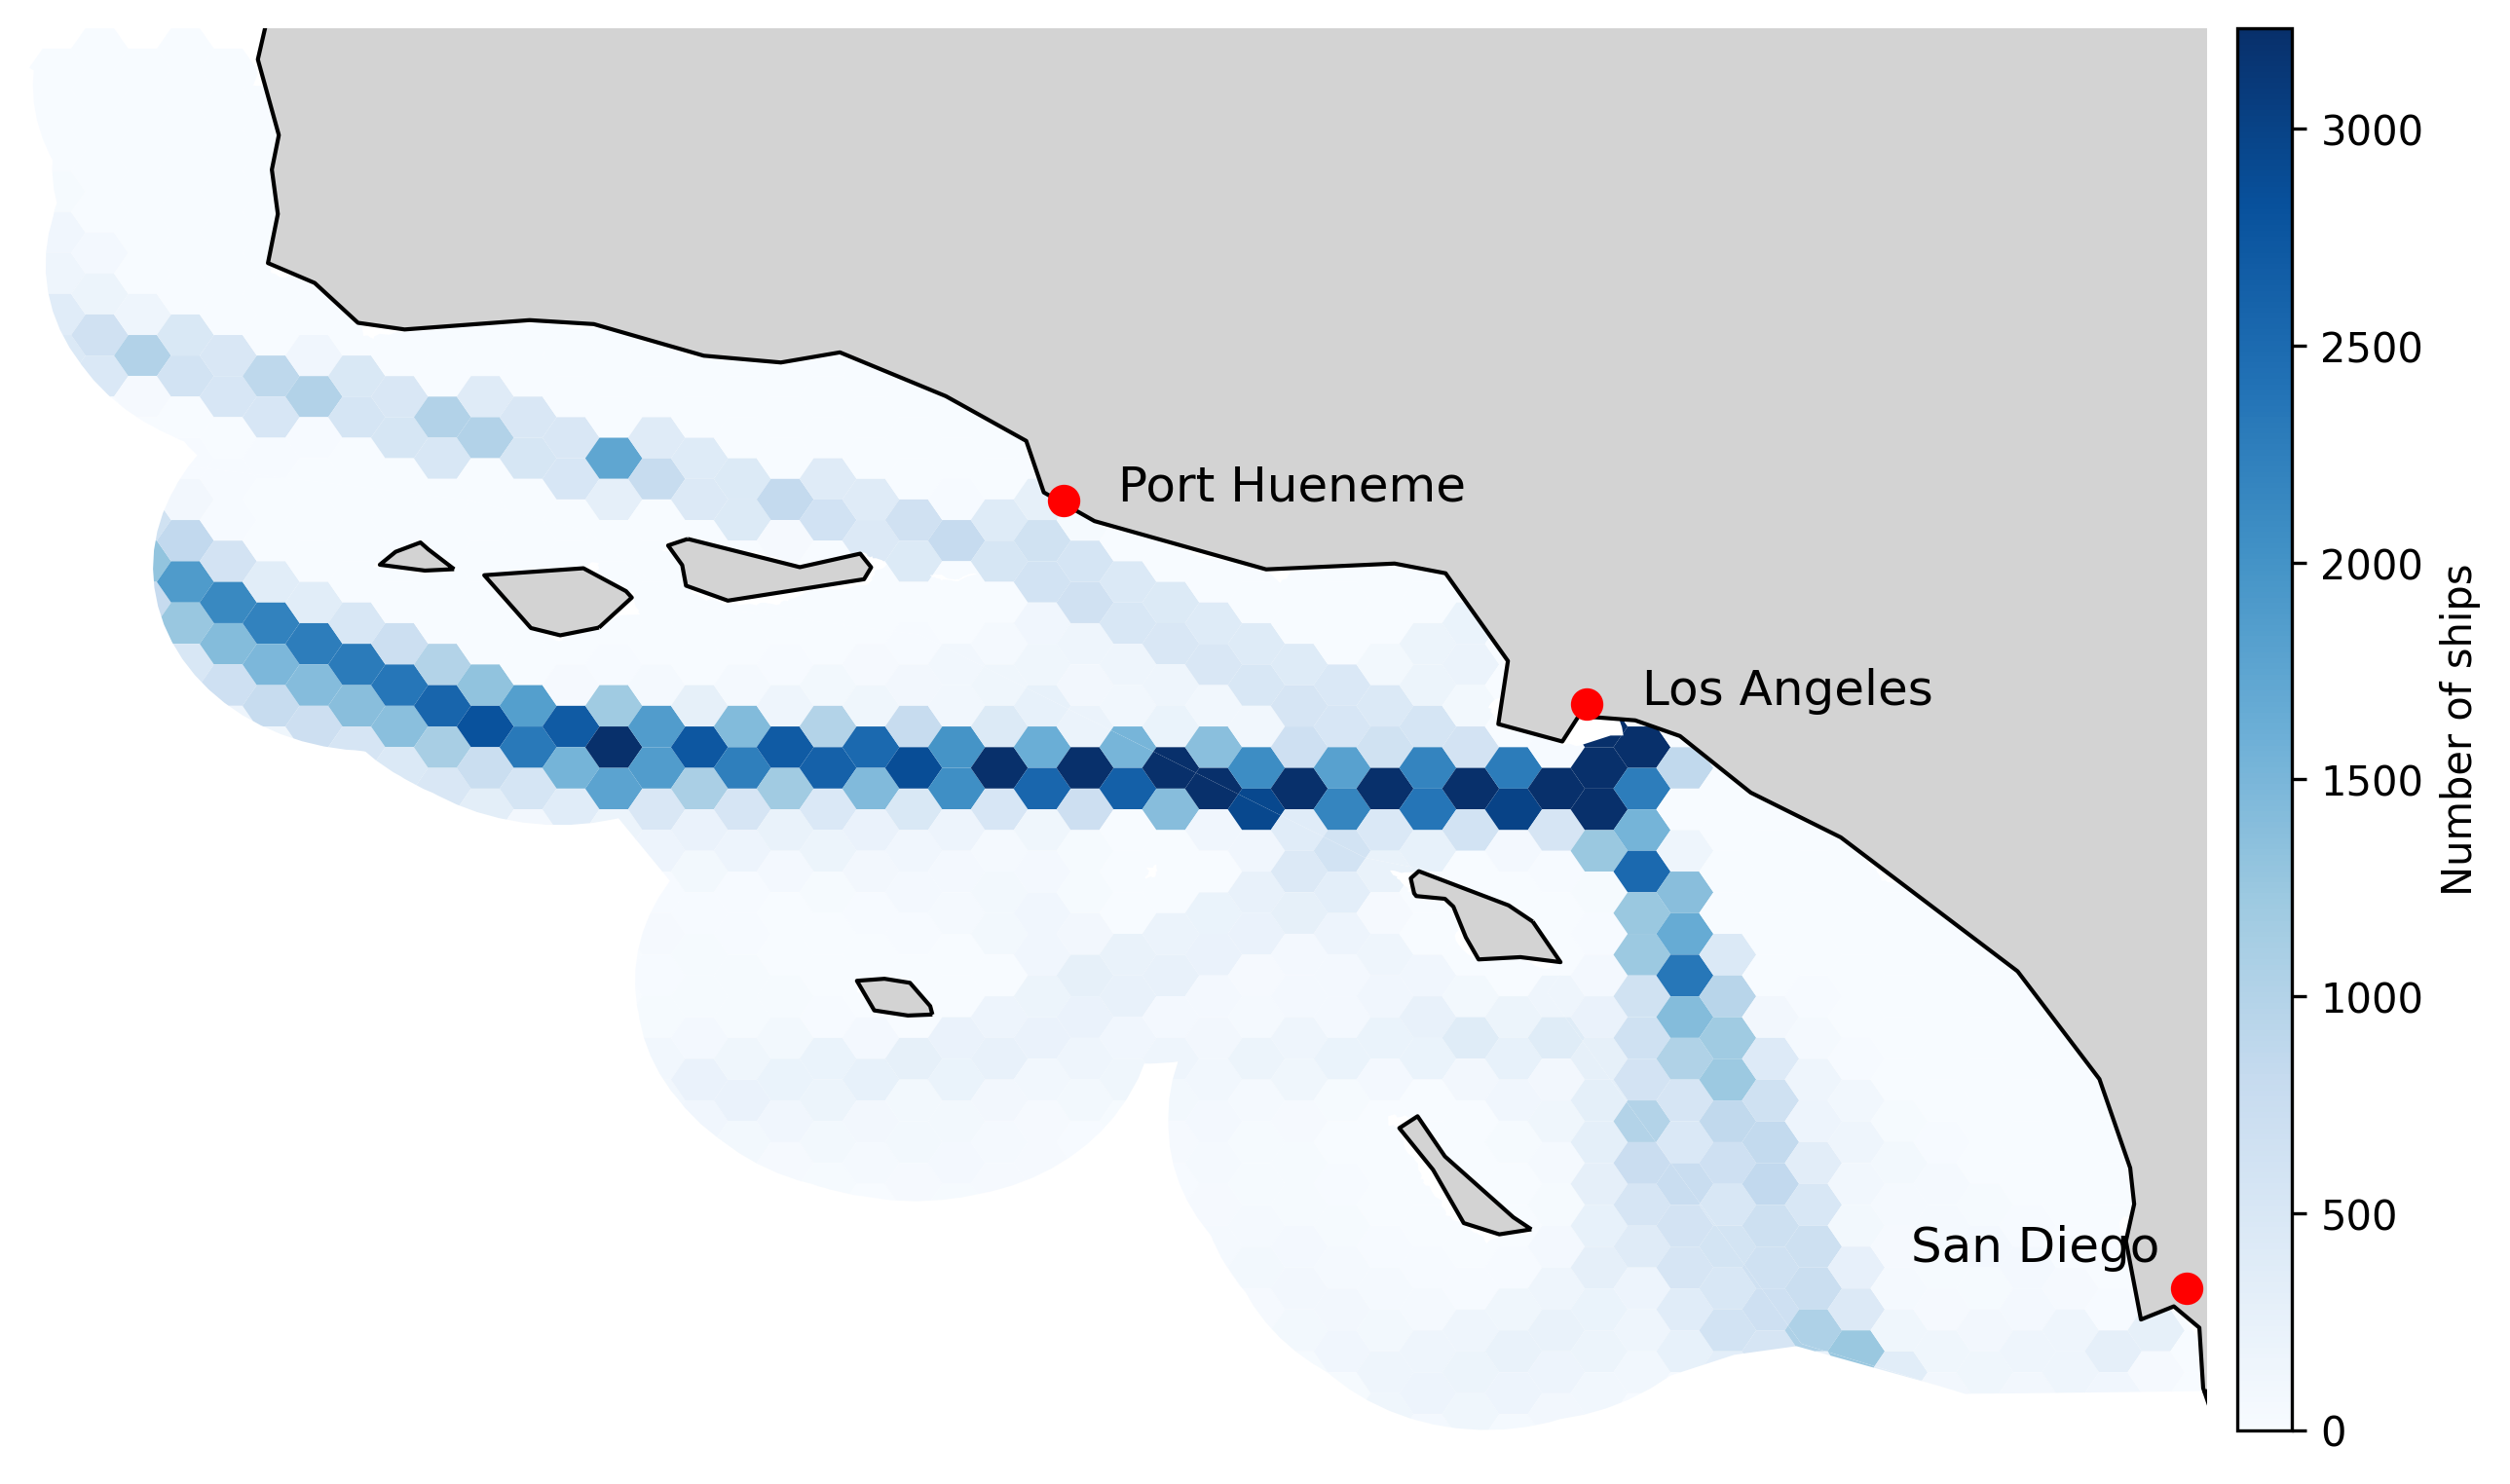
\includegraphics[width=0.8\textwidth]{../output/figures/shipping_exposure_2011.png}
    \caption{Exposure of kelp to maritime traffic in 2011}
    \label{fig:shipping_exposure_2011}
    \vspace{0.5em}
    \begin{flushleft}
{\footnotesize \textit{Notes:} Number of vessel passages through each 10\,km hexagonal cell in Southern California during 2011. The boundary modification took effect in December 2011, so the map overwhelmingly reflects pre-modification routing. Data source: AIS.}
    \end{flushleft}
\end{figure}

\hyperref[appendix_after_2011]{Appendix~\ref*{appendix_after_2011}} provides direct evidence of this redistribution. AIS cell-level data show a shift in total vessel distance between the 2009 zone and the boundary modification area (Figure~\ref{fig:graph_exposure}), consistent with the route adjustments documented in \citet{Klotz2022}.

\subsection{Empirical strategy}

To exploit the 2011 boundary modification, we implement a continuous difference-in-differences design that parallels Eq.~(\ref{eq:cdid}). As in the 2009 specification, the treatment intensity is measured by shipping activity---now from the pre-modification period. The logic is analogous: kelp cells that were more exposed to vessel traffic before the 2011 boundary change should experience worse outcomes afterward if the reallocation of traffic into those corridors increased nearshore stressors.

Specifically, we measure shipping exposure over the full calendar year 2011 using total distance traveled and vessel count within a 20\,km buffer around each kelp hexagon. Because the boundary modification took effect in December 2011---the last month of the year---eleven out of twelve months in our treatment variable reflect pre-modification routing patterns. The remaining month contributes roughly 8\% of the annual average: NBIC vessel arrival records for California ports over 2005--2016 show that December ranks sixth out of twelve months, with a traffic share (8.4\%) virtually identical to the uniform benchmark (8.3\%). Any contamination from post-modification routing in December would blur the spatial contrast between high- and low-exposure cells---mixing pre- and post-modification patterns---thereby attenuating $\gamma$ toward zero rather than inflating it. The 2011 treatment variable is therefore overwhelmingly predetermined and, to the extent it is not, the resulting bias works against our finding. As a direct check, \hyperref[appendix_2010treat]{Appendix~\ref*{appendix_2010treat}} replaces the 2011 treatment with shipping exposure measured during 2010---a year entirely preceding the boundary modification. All coefficients remain negative and significant at the 1\% level, confirming that the results are not driven by the inclusion of December 2011 in the treatment variable. \hyperref[appendix_treat_corr]{Appendix~\ref*{appendix_treat_corr}} documents the correlation between the 2009 and 2011 treatment variables, confirming that the boundary modification generated partially independent spatial variation in shipping exposure.

We estimate:
\begin{equation}
Kelp_{it}=\exp\!\left(\gamma\,Exposure_{i}^{2011}\times \mathit{Post2011}_{t}+\delta\,Z_{it}+f_{i}+f_{t}\right)\cdot\eta_{it},
\label{eq:cdid2011}
\end{equation}
where $Kelp_{it}$ is the sum of kelp biomass (kg) or canopy area (m$^{2}$) in hexagonal cell $i$ during quarter $t$. $Exposure_{i}^{2011}$ is the log of pre-modification shipping intensity measured during 2011 (total distance traveled or vessel count within a 20\,km buffer zone). $\mathit{Post2011}_{t}$ equals one from 2012Q1 onward and zero otherwise (the boundary modification took effect in December 2011, so 2011 quarters are coded as pre-treatment). $Z_{it}$ is defined as in Eq.~(\ref{eq:cdid}). $f_{i}$ denotes kelp-cell fixed effects (defined as in Eq.~(\ref{eq:cdid})) and $f_{t}$ year--quarter fixed effects.

As in Eq.~(\ref{eq:cdid}), the cell fixed effects absorb the main effect of $Exposure_{i}^{2011}$ and any other time-invariant determinant of kelp outcomes; the year--quarter fixed effects absorb common shocks, including the main effect of $\mathit{Post2011}_{t}$. The equation is estimated by PPML, as in the main 2009 specification. Standard errors are clustered at the cell level. The sample covers Southern California (latitudes 32\textdegree--36\textdegree N) from 2005 to 2016, matching the 2009 specification. The year--quarter fixed effects absorb any coast-wide ecological shock, including the 2013--2016 warming episode; such a shock would bias $\gamma$ only if its spatial footprint were systematically correlated with the 2011 shipping-exposure cross-section, for which there is no ecological basis.

The coefficient of interest is $\gamma$. A negative $\gamma$ indicates that, after the 2011 boundary modification, kelp outcomes deteriorated disproportionately in cells that were more exposed to shipping before the policy change---consistent with the reallocation of traffic into those corridors worsening local maritime pressures.

This specification offers a key advantage over an alternative approach that would interact time-varying shipping exposure with a post-2011 indicator: the predetermined nature of $Exposure_{i}^{2011}$ eliminates the concern that contemporaneous vessel routing responds to unobserved marine conditions that also affect kelp. The design thus shares the same identification logic as our main 2009 specification, providing internal consistency across the two natural experiments.

\subsection{Results}

Table~\ref{tab:cdid2011} reports estimates of Eq.~(\ref{eq:cdid2011}). Columns~(1)--(2) measure exposure by total distance traveled by vessels (``Distance Traveled (km)''), with biomass and canopy area as dependent variables respectively. Columns~(3)--(4) measure exposure by vessel count (``Vessel Count'').

\begin{table}[H]
  \centering
  \caption{Continuous difference-in-differences: Kelp outcomes and the 2011 boundary modification}
  \label{tab:cdid2011}
  {
\def\sym#1{\ifmmode^{#1}\else\(^{#1}\)\fi}
\begin{tabular}{l*{4}{c}}
\hline\hline
                    &\multicolumn{2}{c}{Distance Traveled} &\multicolumn{2}{c}{Vessel Count}           \\\cmidrule(lr){2-3}\cmidrule(lr){4-5}
                    &\multicolumn{1}{c}{(1)}&\multicolumn{1}{c}{(2)}&\multicolumn{1}{c}{(3)}&\multicolumn{1}{c}{(4)}\\
                    &\multicolumn{1}{c}{Biomass}&\multicolumn{1}{c}{Area}&\multicolumn{1}{c}{Biomass}&\multicolumn{1}{c}{Area}\\
\hline
Post 2011 $\times$ Exposure&     -0.0925\sym{***}&     -0.0914\sym{***}&      -0.210\sym{***}&      -0.208\sym{***}\\
                    &    (0.0288)         &    (0.0282)         &    (0.0433)         &    (0.0425)         \\
[1em]
SST                 &      -7.155\sym{***}&      -7.060\sym{***}&      -7.103\sym{***}&      -7.008\sym{***}\\
                    &     (0.904)         &     (0.909)         &     (0.903)         &     (0.908)         \\
[1em]
Precipitation       &     -0.0359         &     -0.0386         &     -0.0483         &     -0.0508         \\
                    &    (0.0781)         &    (0.0773)         &    (0.0782)         &    (0.0776)         \\
[1em]
Significant Wave Height&      -3.452\sym{***}&      -3.371\sym{***}&      -3.341\sym{***}&      -3.262\sym{***}\\
                    &     (0.958)         &     (0.951)         &     (0.956)         &     (0.949)         \\
\hline
Cell FE             &         Yes         &         Yes         &         Yes         &         Yes         \\
Year-Quarter FE     &         Yes         &         Yes         &         Yes         &         Yes         \\
Observations        &        6000         &        6000         &        6000         &        6000         \\
\hline\hline
\end{tabular}
}

  \vspace{0.5em}

  \begin{minipage}{\linewidth}
  \footnotesize
  \textit{Notes:} Unweighted PPML estimates of Eq.~(\ref{eq:cdid2011}). The dependent variable is kelp biomass (kg) or canopy area (m$^{2}$). ``Distance Traveled (km)'' columns~(1)--(2) measure exposure by logged total distance traveled by vessels within a 20\,km buffer around each kelp hexagon during 2011; ``Vessel Count'' columns~(3)--(4) use the corresponding logged vessel count. All specifications include kelp-cell and year--quarter fixed effects. Standard errors clustered at the cell level (125 clusters) in parentheses. Sample: Southern California (32\textdegree--36\textdegree\,N), 2005--2016, 6,000 observations (125 cells $\times$ 48 quarters). Weighted estimates, which are qualitatively identical, are reported in \hyperref[appendix_weighted_2011]{Appendix~\ref*{appendix_weighted_2011}}.\\
  \sym{*} \(p<0.10\), \sym{**} \(p<0.05\), \sym{***} \(p<0.01\).
  \end{minipage}
\end{table}

Across all specifications, the interaction between post-2011 implementation and pre-modification shipping exposure is negative and statistically significant at the 1\% level. The estimates are stable across treatment-intensity measures and dependent variables.

In columns~(1)--(2), which use logged distance traveled by vessels, the coefficient of approximately $-0.093$ implies that a one-unit increase in log pre-2011 distance traveled is associated with a $1-\exp(-0.093)\approx 8.9\%$ larger post-2011 decrease in expected kelp biomass and canopy. In columns~(3)--(4), the coefficient on logged vessel count is approximately $-0.210$, implying a $1-\exp(-0.210)\approx 18.9\%$ relative decline per unit of log vessel count.

These results are the mirror image of the 2009 findings in Table~\ref{tab:main_2009}. Where the 2009 regulation was associated with disproportionate kelp improvement in high-exposure cells ($\hat{\beta}>0$), the 2011 boundary modification was associated with disproportionate kelp deterioration in cells exposed to re-concentrated traffic ($\hat{\gamma}<0$). The symmetry of these two findings---one following a regulation that tightened fuel standards for nearshore shipping, the other following a boundary change that redirected traffic into new corridors---strengthens the causal interpretation: maritime regulation has a quantitatively important and plausibly causal effect on kelp forest health, mediated by changes in the spatial footprint of vessel activity.

Environmental controls enter with expected signs and are consistent with the estimates in Table~\ref{tab:main_2009}. Sea surface temperature is strongly and negatively associated with kelp outcomes ($-7.2$ to $-7.0$), confirming kelp sensitivity to warm-water conditions. Significant wave height is also strongly negative ($-3.5$ to $-3.3$), reflecting physical stress from storms. Precipitation is positive but statistically insignificant.

\subsection{Dynamic effects}

A standard PPML event study for the 2011 boundary modification faces a specific identification challenge: the 2009 ECA regulation, which constitutes the main treatment in the first part of this paper, falls within the pre-treatment window for the 2011 event. Because both treatments rely on cross-sectional variation in shipping intensity, a conventional two-way fixed-effects event study cannot disentangle the 2009 and 2011 effects---the pre-2011 coefficients would reflect a mix of the 2009 treatment dynamics and genuine pre-trends for the 2011 shock.

To address this, we implement the heterogeneity-robust estimator of \citet{Chaisemartin2024}, which accommodates continuous (non-binary) treatments. The treatment variable $D_{it}^{2011}$ equals zero for all cells before 2011 and equals the log of mean vessel distance traveled within a 20\,km buffer (measured in 2011) from 2011 onward. The key identifying assumption is that, in the absence of the 2011 shock, the evolution of kelp outcomes would have been linear in the cross-sectional shipping intensity. The estimator fits this baseline trend from the earliest pre-treatment period and uses it to project counterfactual outcomes at each event time; deviations from this projection are the estimated treatment effects. Because the treatment variable is identically zero before 2011, the cross-sectional variation that identifies the baseline polynomial comes from the relationship between shipping intensity and kelp trends during the pre-treatment years, not from variation in the treatment itself.

The panel is collapsed to annual frequency to avoid seasonal heteroscedasticity in quarterly kelp data---winter quarters (Q1, Q4) exhibit roughly ten times smaller variance than spring/summer quarters (Q2, Q3), which would distort the apparent precision of quarterly event-study coefficients. The sample covers 2008--2016, with the first pre-treatment year (2008) used to fit the baseline polynomial, leaving two pre-treatment placebos (2009, 2010) and six post-treatment effects (2011--2016). Standard errors are obtained by bootstrap (999 replications) clustered at the cell level.

\begin{figure}[H]
    \centering
    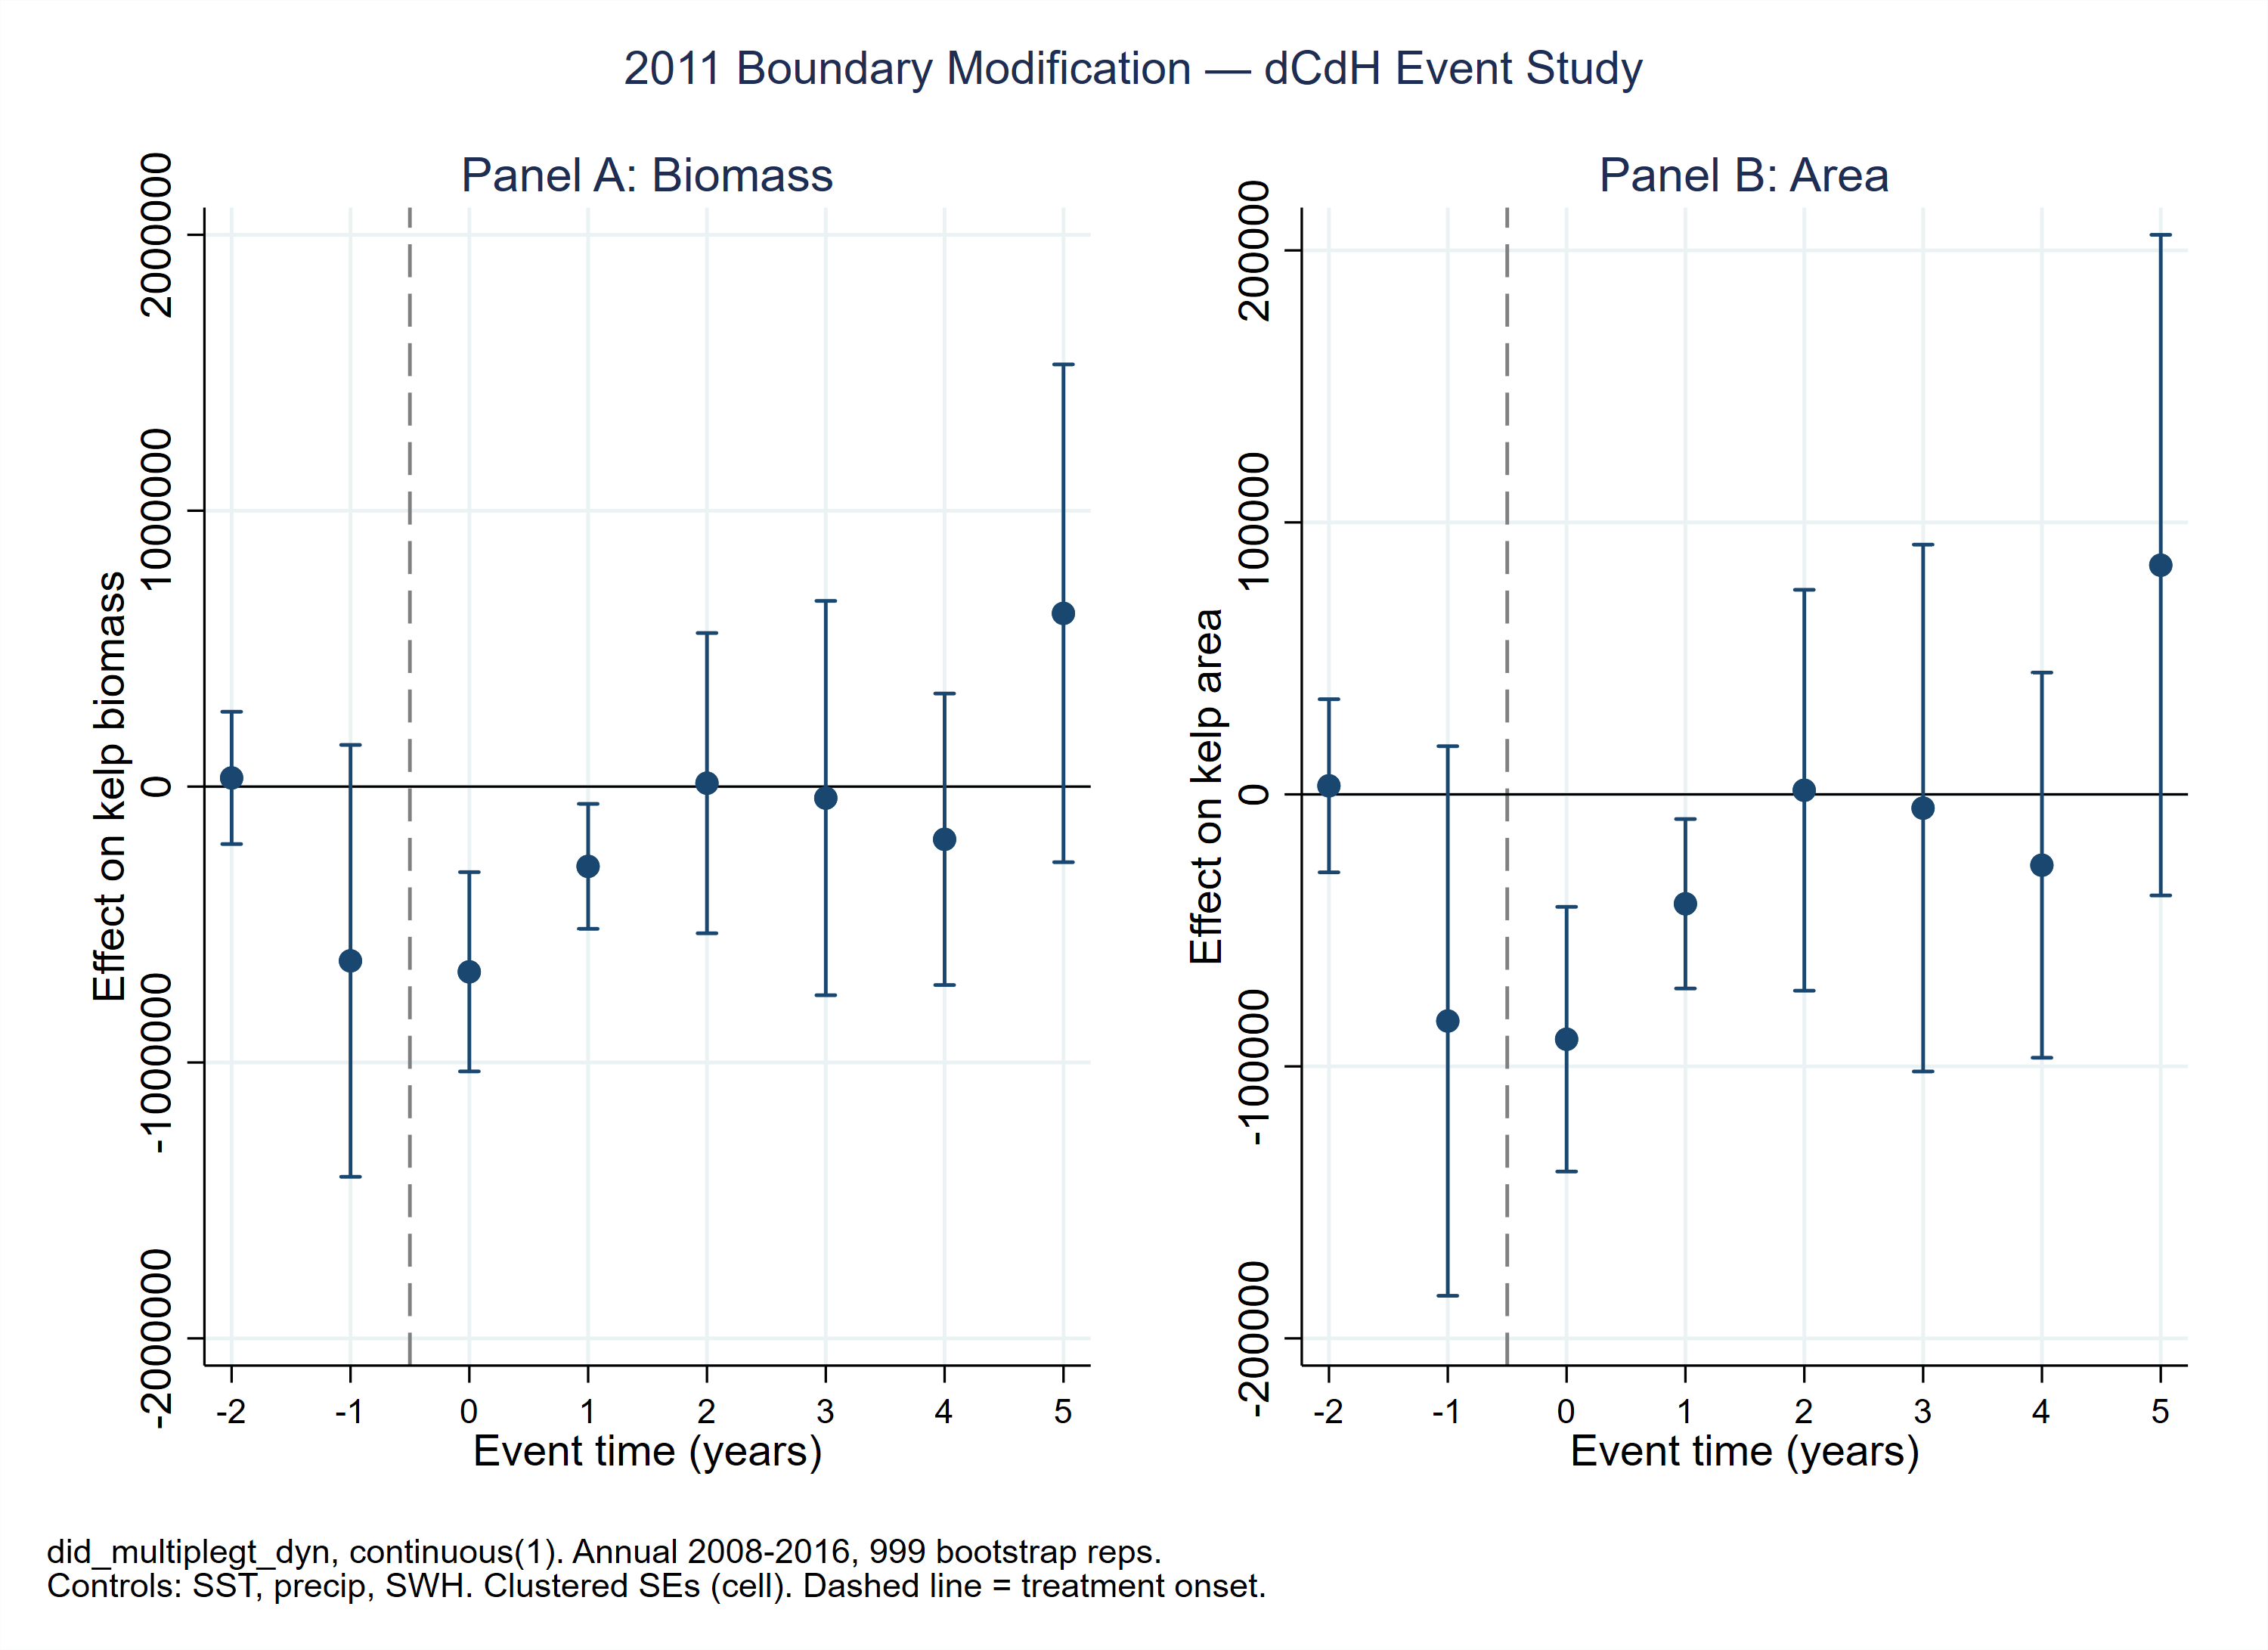
\includegraphics[width=0.95\textwidth]{../output/figures/event_study_2011_dCdH.png}
    \caption{Event study: 2011 boundary modification (de Chaisemartin--D'Haultf\oe uille estimator)}
    \label{fig:event_study_2011_dCdH}
    \vspace{0.15em}
    \begin{flushleft}
        \footnotesize Note: Each panel plots heterogeneity-robust treatment effects from the \texttt{did\_multiplegt\_dyn} estimator of \citet{Chaisemartin2024} with continuous treatment intensity (linear polynomial). The treatment variable is zero before 2011 and equals log mean vessel distance within a 20\,km buffer from 2011 onward. The panel is annual (2008--2016). Controls: log SST, log precipitation, log significant wave height. Error bars are 95\% bootstrap confidence intervals (999 replications, clustered at the cell level). Panel~A: kelp biomass; Panel~B: kelp canopy area. Dashed line marks treatment onset.
    \end{flushleft}
\end{figure}

Figure~\ref{fig:event_study_2011_dCdH} presents the results. Both pre-treatment placebos (event times $-2$ and $-1$, corresponding to 2009 and 2010) are statistically insignificant, with confidence intervals comfortably crossing zero, supporting the parallel-trends assumption for the 2011 shock even in the presence of the concurrent 2009 regulation.\footnote{The event time $-1$ point estimate is negative in the biomass panel, but the wide confidence interval ($p>0.10$) is consistent with sampling variation rather than a pre-trend.} Following the 2011 boundary modification, the treatment effect turns sharply negative at event times~0 and~1, indicating that cells more exposed to shipping experienced a deterioration in kelp outcomes. By event times~2--5 (2013--2016), the point estimates gradually return toward zero, indicating that the negative effect was transitory. This pattern is consistent with kelp's well-documented capacity for rapid regrowth---giant kelp (\textit{Macrocystis pyrifera}) can grow 30--60\,cm per day under favorable conditions---consistent with partial ecological recovery, though other time-varying factors may also contribute.

This dynamic pattern complements the static PPML estimates in Table~\ref{tab:cdid2011}. While the static specification pools all post-2011 periods and estimates the average effect under PPML, the event study traces the temporal evolution under OLS with the heterogeneity-robust corrections of \citet{Chaisemartin2024}. The transitory nature of the effect implies that the static estimate, which averages over both the initial damage and subsequent recovery, understates the short-run impact of the boundary modification. Nevertheless, the convergence of both approaches---different estimators, different functional forms---reinforces the conclusion that the 2011 boundary modification worsened kelp outcomes in high-shipping cells, even if the ecosystem partially recovered.

The transitory nature of the 2011 effect contrasts with the persistent 2009 effect, which shows no attenuation through 2016. This asymmetry has a natural biological explanation. The transitory 2011 effect reflects kelp's capacity for rapid regrowth: once the initial damage from re-concentrated traffic is absorbed, giant kelp can recolonize, closing the gap between high- and low-exposure cells within a few years. The persistent 2009 effect, by contrast, is consistent with a sustained change in nearshore conditions: as long as the regulation remains in force, the conditions favoring kelp recovery in formerly high-exposure cells persist, so the positive differential does not attenuate.

\section{Conclusion}

\begin{quotation}
``If in any country a forest was destroyed, I do not believe as many species of animals would perish as would here from the destruction of kelp.'' --- \citet{Darwin1839}
\end{quotation}
Human reliance on kelp dates back to prehistoric times; \citet{Erlandson2007} even propose a ``Kelp Highway Hypothesis’’ explaining that human migration 20,000 years ago depended on this resource. Yet these same kelp corridors are now traversed by giant vessels that leave maritime pollution in their wake.

In this paper, we have exploited two policy episodes---the 2009 Ocean-Going Vessel Fuel Rule and the 2011 boundary modification around the Channel Islands---to estimate the causal effect of maritime regulation on kelp forests along the California coast, operating through differential shipping exposure. Using a continuous difference-in-differences design with shipping-specific exposure measures derived from AIS vessel trajectories, we show that (i)~kelp canopy and biomass improved disproportionately in cells more exposed to vessel traffic after the 2009 regulation tightened fuel standards for nearshore vessels, and (ii)~kelp deteriorated disproportionately in cells more exposed to shipping before the 2011 boundary change re-concentrated traffic in specific corridors. Event-study diagnostics show approximately flat pre-trends for shipping-specific measures in the 2009 specification (Figure~\ref{fig:event_study_main}), while broader cumulative impact measures exhibit significant pre-trends driven by non-shipping confounders. For the 2011 episode, a heterogeneity-robust event study \citep{Chaisemartin2024} likewise shows no pre-trend despite the concurrent 2009 regulation (Figure~\ref{fig:event_study_2011_dCdH}), and reveals that the negative effect was transitory---kelp partially recovered within two to three years, consistent with the rapid regrowth capacity of giant kelp. The symmetry of the 2009 and 2011 results---one following a tightening of fuel standards, the other following a spatial reallocation of traffic---strengthens the causal interpretation that maritime activity has a quantitatively important effect on kelp forest health, operating through channels that covary with the spatial footprint of maritime activity, which the regulation altered through both fuel switching and route adjustments.

These findings have implications for both economic analysis and maritime policy. First, as the international trade literature now examines the ``hidden costs’’ of globalization, we bring kelp forests into this discussion: they play an important role in fisheries, alginate production, and carbon sequestration in coastal ecosystems. An illustrative back-of-the-envelope calculation suggests that the ECA-induced kelp improvement in our study area is worth on the order of \$59--67 million per year in ecosystem services---a figure not currently reflected in cost-benefit assessments of maritime emission regulation.\footnote{We apply the ecosystem service valuations of \citet{Eger2023}, who estimate that \textit{Macrocystis} kelp forests provide approximately \$72,000/ha/year through fisheries production, nutrient cycling, and carbon sequestration. Our study area contains roughly 5,500 hectares of kelp canopy (pre-period annual mean). Multiplying by the approximately 15--17\% improvement implied by the main estimates yields approximately \$59--67 million per year. This calculation is approximate: it assumes that the average treatment intensity across cells maps one-to-one onto the semi-elasticity, and it relies on global average per-hectare valuations rather than California-specific estimates.}

Second, this study supports the objectives of the International Maritime Organization (IMO), which has been pivotal in enforcing emission control areas over the past decade. In settings where regulated zones overlap with nearshore ecosystems, ECAs may have effects beyond their impact on air pollution, and could play a role in promoting sustainable international trade that limits damage to coastal habitats. At the same time, the 2011 episode serves as a cautionary finding: boundary modifications that re-concentrate traffic can undo some of the environmental benefits of the original regulation, suggesting that spatial design matters as much as the stringency of emission standards.

\printbibliography
\newpage

\appendix


\section{Weighting Robustness and Cumulative Impact Index: the 2009 ECA}\label{appendix_weighted}

The main specification uses unweighted PPML on the restricted sample of 81 cells recording at least two vessel passages per month on average. This appendix examines robustness to alternative weighting schemes and to an alternative treatment measure.

Table~\ref{tab:weighted_2009} reports weighted PPML estimates on the same restricted sample, using log vessel count as observation weight (offset trick; see \citealp{Solon2015} for a discussion of weighting motives in regression). The coefficients are virtually identical to the unweighted estimates in Table~\ref{tab:main_2009}: 0.135 versus 0.136 for vessel distance and 0.152 versus 0.155 for vessel count, all significant at the 1\% level. This stability confirms that the results are not sensitive to the weighting scheme once cells with negligible shipping exposure are excluded.

\begin{table}[H]
  \centering
  \caption{Weighted PPML: Kelp outcomes and the 2009 ECA}
  \label{tab:weighted_2009}
  \def\sym#1{\ifmmode^{#1}\else\(^{#1}\)\fi}
\begin{tabular}{l*{4}{c}}
\hline\hline
                    &\multicolumn{2}{c}{Distance Traveled (km)}&\multicolumn{2}{c}{Vessel Count}\\
                    \cmidrule(lr){2-3}\cmidrule(lr){4-5}
                    &\multicolumn{1}{c}{(1)}&\multicolumn{1}{c}{(2)}&\multicolumn{1}{c}{(3)}&\multicolumn{1}{c}{(4)}\\
                    &\multicolumn{1}{c}{Biomass}&\multicolumn{1}{c}{Area}&\multicolumn{1}{c}{Biomass}&\multicolumn{1}{c}{Area}\\
\hline
Post 2009 $\times$ Exposure&     0.1352\sym{***}&     0.1308\sym{***}&     0.1517\sym{***}&     0.1463\sym{***}\\
                    &             (0.0372)&             (0.0366)&             (0.0446)&             (0.0439)\\
[1em]
SST                 &     -5.364\sym{***}&     -5.194\sym{***}&     -5.387\sym{***}&     -5.216\sym{***}\\
                    &              (1.176)&              (1.161)&              (1.181)&              (1.167)\\
[1em]
Precipitation       &     0.0842&     0.0899&     0.0911&     0.0965\\
                    &             (0.1093)&             (0.1065)&             (0.1100)&             (0.1071)\\
[1em]
Significant Wave Height&     -3.426\sym{**}&     -3.278\sym{**}&     -3.495\sym{**}&     -3.345\sym{**}\\
                    &              (1.538)&              (1.512)&              (1.541)&              (1.513)\\
[1em]
\hline
Cell FE             &         Yes         &         Yes         &         Yes         &         Yes         \\
Year-Quarter FE     &         Yes         &         Yes         &         Yes         &         Yes         \\
Observations        &        3880         &        3880         &        3880         &        3880         \\
\hline\hline
\end{tabular}
  \vspace{0.5em}

  \begin{minipage}{\linewidth}
  \footnotesize
  \textit{Notes:} Weighted PPML estimates of Eq.~(\ref{eq:cdid}). The dependent variable is kelp biomass (kg) or canopy area (m$^{2}$). ``Distance Traveled (km)'' columns~(1)--(2) measure exposure by logged mean distance traveled by vessels within a 20\,km buffer during January--June 2009; ``Vessel Count'' columns~(3)--(4) use the corresponding logged mean vessel count. Observations weighted by log vessel count (offset trick). All specifications include kelp-cell and year--quarter fixed effects. Sample: Southern California (32\textdegree--36\textdegree\,N), 2005--2016, restricted to cells with at least two vessel passages per month on average (81 cells, 3,880 observations). Standard errors clustered at the cell level (81 clusters) in parentheses.\\
  \sym{*} \(p<0.10\), \sym{**} \(p<0.05\), \sym{***} \(p<0.01\).
  \end{minipage}
\end{table}

As a complementary exercise, we replace the AIS-based treatment with the cumulative human impact index of \citet{Halpern2009}, which aggregates 25 anthropogenic stressors into a single measure. The coefficient is positive and significant, but event-study diagnostics reveal severe violations of the parallel-trends assumption (pre-policy coefficients of $-0.18$ to $-0.14$, all significant at the 1\% level; joint Wald test $p<0.001$). These pre-trends are driven by non-shipping stressors bundled in the index, motivating our preference for shipping-specific AIS measures.

\paragraph{Sensitivity to sample restriction.} Figure~\ref{fig:weighting_diagnostic} traces the coefficient as a function of an increasingly restrictive sample cutoff. The estimate stabilizes once cells with negligible shipping exposure are excluded, confirming that the baseline restriction removes noise from cells where the treatment variable captures geographic features rather than policy-relevant variation.

\begin{figure}[H]
  \centering
  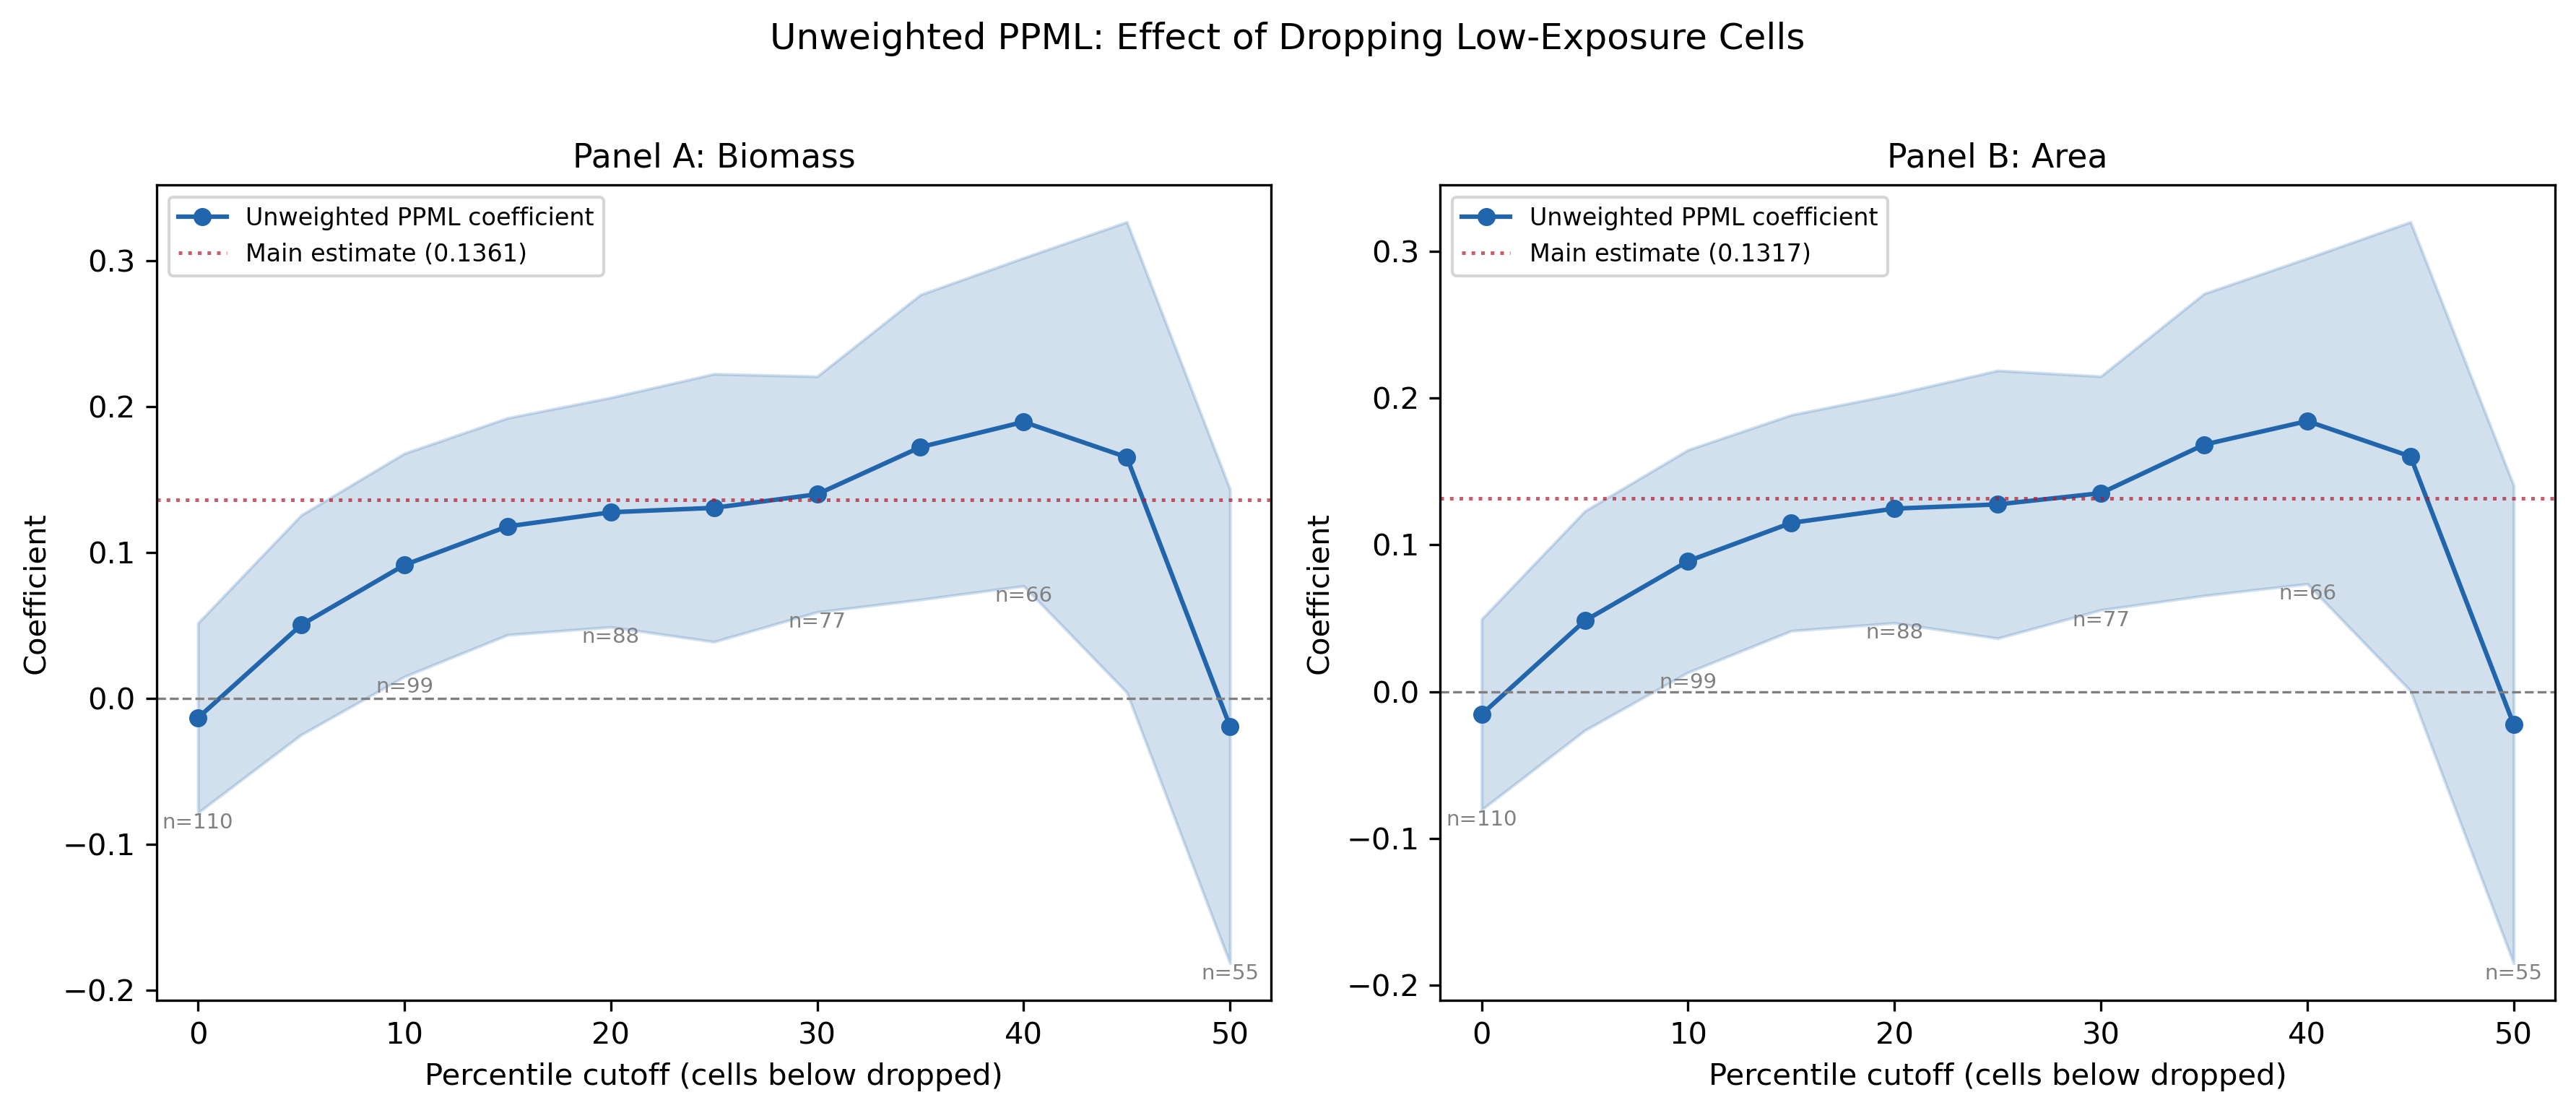
\includegraphics[width=\textwidth]{../output/figures/weighting_diagnostic.png}
  \caption{PPML coefficient as a function of sample restriction}
  \label{fig:weighting_diagnostic}
  \vspace{0.5em}
  \begin{minipage}{\linewidth}
  \footnotesize
  \textit{Notes:} Each point reports the unweighted PPML coefficient from Eq.~(\ref{eq:cdid}) estimated on the subsample of cells above the indicated percentile of pre-policy shipping exposure (logged mean vessel distance). Cutoffs range from the 5th to the 50th percentile. The shaded area shows 95\% confidence intervals based on standard errors clustered at the cell level. The horizontal dashed line marks the main estimate for each dependent variable. The number of cells in each subsample is indicated below the confidence band. Sample: Southern California, 2005--2016.
  \end{minipage}
\end{figure}

Table~\ref{tab:weighting_robustness} confirms this pattern across alternative specifications. Panel~A reproduces the main unweighted estimate. Panel~B applies vessel count weights (offset trick) on the same restricted sample; the coefficients are nearly identical. Panel~C uses pre-period kelp biomass (2005--2008 average) as an alternative weight, capturing the ecological size of each cell rather than its shipping exposure; all four coefficients remain positive and significant at the 1\% level.

\begin{table}[H]
  \centering
  \caption{Weighting robustness: alternative specifications}
  \label{tab:weighting_robustness}
  \def\sym#1{\ifmmode^{#1}\else\(^{#1}\)\fi}
\begin{tabular}{l*{4}{c}}
\hline\hline
                    &\multicolumn{2}{c}{Distance Traveled (km)}&\multicolumn{2}{c}{Vessel Count}\\
                    \cmidrule(lr){2-3}\cmidrule(lr){4-5}
                    &\multicolumn{1}{c}{(1)}&\multicolumn{1}{c}{(2)}&\multicolumn{1}{c}{(3)}&\multicolumn{1}{c}{(4)}\\
                    &\multicolumn{1}{c}{Biomass}&\multicolumn{1}{c}{Area}&\multicolumn{1}{c}{Biomass}&\multicolumn{1}{c}{Area}\\
\hline
\multicolumn{5}{l}{\textit{Panel A: Main specification (unweighted PPML)}}\\[0.3em]
Post 2009 $\times$ Exposure&     0.1361\sym{***}&     0.1317\sym{***}&     0.1548\sym{***}&     0.1493\sym{***}\\
                    &             (0.0359)&             (0.0352)&             (0.0432)&             (0.0424)\\
Observations        &        3880         &        3880         &        3880         &        3880         \\
[1em]
\multicolumn{5}{l}{\textit{Panel B: Weighted by vessel count (offset trick)}}\\[0.3em]
Post 2009 $\times$ Exposure&     0.1352\sym{***}&     0.1308\sym{***}&     0.1517\sym{***}&     0.1463\sym{***}\\
                    &             (0.0372)&             (0.0366)&             (0.0446)&             (0.0439)\\
Observations        &        3880         &        3880         &        3880         &        3880         \\
[1em]
\multicolumn{5}{l}{\textit{Panel C: Weighted by pre-period kelp biomass}}\\[0.3em]
Post 2009 $\times$ Exposure&     0.1029\sym{***}&     0.0995\sym{***}&     0.1242\sym{***}&     0.1196\sym{***}\\
                    &             (0.0296)&             (0.0286)&             (0.0382)&             (0.0365)\\
Observations        &        3736         &        3736         &        3736         &        3736         \\
Controls            &         Yes         &         Yes         &         Yes         &         Yes         \\
Cell FE             &         Yes         &         Yes         &         Yes         &         Yes         \\
Year-Quarter FE     &         Yes         &         Yes         &         Yes         &         Yes         \\
\hline\hline
\end{tabular}
  \vspace{0.5em}
  \begin{minipage}{\linewidth}
  \footnotesize
  \textit{Notes:} Panel~A reproduces the main specification from Table~\ref{tab:main_2009} (unweighted PPML on cells with $\geq 2$ vessel passages/month). Panel~B applies vessel count weights (offset trick) on the same restricted sample. Panel~C uses pre-period kelp biomass (2005--2008 cell-level average) as observation weight; 3 cells with zero pre-period kelp are dropped. All specifications include kelp-cell and year--quarter fixed effects. Controls: log sea surface temperature, log precipitation, log significant wave height. Standard errors clustered at the cell level in parentheses.\\
  \sym{*} \(p<0.10\), \sym{**} \(p<0.05\), \sym{***} \(p<0.01\).
  \end{minipage}
\end{table}

\newpage

\section{Placebo Test for the 2009 ECA}\label{appendix_placebo}

A natural concern with the main results is that the positive post-2009 coefficient might reflect a pre-existing differential trend rather than a causal effect of the ECA regulation. To address this, we conduct a placebo test by assigning a fictitious treatment date within the pre-policy period and verifying that no significant effect is detected.

Specifically, we restrict the sample to the pre-policy years 2005--2008 and define a fake ``post'' indicator equal to one from 2007Q3 onward (and zero before). We then re-estimate Eq.~(\ref{eq:cdid}) using the same PPML specification as in the main analysis: the same treatment variables (vessel distance and vessel count), the same controls (SST, precipitation, significant wave height), and the same cell and year--quarter fixed effects. The only difference is that the genuine post-2009 indicator is replaced by the fake 2007Q3 indicator, and the sample contains no post-regulation observations.

Table~\ref{tab:placebo} reports the results. All four placebo coefficients are small, negative, and statistically insignificant, with $p$-values ranging from 0.26 to 0.30. This stands in sharp contrast to the main estimates in Table~\ref{tab:main_2009}, where the coefficients are positive and significant ($+0.136$ for vessel distance, $+0.155$ for vessel count, both $p<0.01$). The placebo coefficients are also opposite in sign, ruling out the possibility that any pre-existing positive differential trend drives the main result.

\begin{table}[H]
  \centering
  \caption{Placebo test: Fake treatment date (2007Q3) on pre-policy sample}
  \label{tab:placebo}
  \def\sym#1{\ifmmode^{#1}\else\(^{#1}\)\fi}
\begin{tabular}{l*{4}{c}}
\hline\hline
                    &\multicolumn{2}{c}{Distance Traveled (km)}&\multicolumn{2}{c}{Vessel Count}\\
                    \cmidrule(lr){2-3}\cmidrule(lr){4-5}
                    &\multicolumn{1}{c}{(1)}&\multicolumn{1}{c}{(2)}&\multicolumn{1}{c}{(3)}&\multicolumn{1}{c}{(4)}\\
                    &\multicolumn{1}{c}{Biomass}&\multicolumn{1}{c}{Area}&\multicolumn{1}{c}{Biomass}&\multicolumn{1}{c}{Area}\\
\hline
Fake Post 2007Q3 $\times$ Exposure&    -0.0753&    -0.0694&    -0.0859&    -0.0804\\
                    &             (0.0673)&             (0.0669)&             (0.0755)&             (0.0749)\\
[1em]
Observations        &        1248         &        1248         &        1248         &        1248         \\
Controls            &         Yes         &         Yes         &         Yes         &         Yes         \\
Cell FE             &         Yes         &         Yes         &         Yes         &         Yes         \\
Year-Quarter FE     &         Yes         &         Yes         &         Yes         &         Yes         \\
\hline\hline
\end{tabular}

  \vspace{0.5em}
  \begin{minipage}{\linewidth}
  \footnotesize
  \textit{Notes:} PPML estimates of Eq.~(\ref{eq:cdid}) with a fictitious treatment date set at 2007Q3 on the pre-policy sample (2005--2008 only). The dependent variable is kelp biomass (kg) or canopy area (m$^{2}$). ``Distance Traveled (km)'' columns~(1)--(2) measure exposure by logged mean distance traveled by vessels within a 20\,km buffer during January--June 2009; ``Vessel Count'' columns~(3)--(4) use the corresponding logged mean vessel count. All specifications include kelp-cell and year--quarter fixed effects. Sample restricted to cells with at least two vessel passages per month on average. Standard errors clustered at the cell level in parentheses.\\
  \sym{*} \(p<0.10\), \sym{**} \(p<0.05\), \sym{***} \(p<0.01\).
  \end{minipage}
\end{table}

These results are consistent with the positive effect identified in the main analysis being specific to the actual 2009 ECA enforcement date rather than arising from pre-existing differential trends between high- and low-shipping cells.

\newpage

\section{Balance Table}\label{appendix_balance}

Table~\ref{tab:balance} reports pre-treatment (2005--2008) means of key variables across quartiles of the treatment variable (log vessel distance traveled, January--June 2009). The last column reports the $p$-value from a Kruskal--Wallis test for differences across quartiles.

The treatment variable exhibits strong variation by construction: mean log vessel distance ranges from 9.3 in the lowest quartile to 13.3 in the highest. Vessel count shows a similar gradient. SST, precipitation, and significant wave height all differ significantly across quartiles ($p<0.01$), reflecting geographic sorting---high-shipping cells are concentrated near ports, which tend to be in calmer, warmer waters. These environmental variables are controlled for directly in the regression.

Pre-treatment kelp biomass and canopy area are highest in Q1 (lowest exposure) and decline monotonically with shipping intensity, indicating that high-exposure cells do not have systematically better kelp conditions before the policy. This pattern is reassuring: it rules out the concern that the positive post-2009 coefficient reflects a pre-existing advantage of high-shipping cells.

\begin{table}[H]
  \centering
  \caption{Pre-treatment balance across treatment-intensity quartiles}
  \label{tab:balance}
  \def\sym#1{\ifmmode^{#1}\else\(^{#1}\)\fi}
\begin{tabular}{l*{4}{c}c}
\hline\hline
                    &\multicolumn{1}{c}{Q1 (low)}&\multicolumn{1}{c}{Q2}&\multicolumn{1}{c}{Q3}&\multicolumn{1}{c}{Q4 (high)}&\multicolumn{1}{c}{KW $p$}\\
\hline
Log vessel distance (Jan-Jun 2009)      &       9.311&      10.491&      12.470&      13.321&   0.000\\
                                        &     [0.491]&     [0.290]&     [0.564]&     [0.182]&        \\
[0.5em]
Kelp biomass (kg)                       &   1655116.8&    801416.6&    409706.0&    321770.5&   0.000\\
                                        & [3976548.5]& [2459511.5]&  [929510.4]&  [904773.3]&        \\
[0.3em]
Kelp canopy area (m$^{2}$)              &    220694.5&    107794.3&     54520.6&     43562.9&   0.000\\
                                        &  [521297.4]&  [333245.2]&  [121129.7]&  [123756.5]&        \\
[0.3em]
Log SST                                 &       2.842&       2.883&       2.798&       2.844&   0.000\\
                                        &     [0.134]&     [0.124]&     [0.125]&     [0.124]&        \\
[0.3em]
Log precipitation                       &       2.611&       2.506&       2.779&       2.729&   0.009\\
                                        &     [1.052]&     [1.116]&     [1.221]&     [1.164]&        \\
[0.3em]
Log significant wave height             &      0.8859&      0.7991&      0.8732&      0.7286&   0.000\\
                                        &    [0.1626]&    [0.1313]&    [0.1748]&    [0.1465]&        \\
[0.3em]
Log vessel count (Jan-Jun 2009)         &      0.9722&       1.516&       3.593&       4.300&   0.000\\
                                        &    [0.1562]&     [0.310]&     [0.468]&     [0.134]&        \\
[0.3em]
\hline
Cells                                   &          21&          20&          20&          20&        \\
\hline\hline
\end{tabular}

  \vspace{0.5em}
  \begin{minipage}{\linewidth}
  \footnotesize
  \textit{Notes:} Cell-quarter means during the pre-treatment period (2005--2008), by quartile of log vessel distance traveled (January--June 2009, 20\,km buffer). Standard deviations in brackets. The last column reports the $p$-value from a Kruskal--Wallis test of equality of distributions across quartiles. Sample: 81 cells (20--21 per quartile), Southern California (32\textdegree--36\textdegree\,N), restricted to cells with at least two vessel passages per month on average.
  \end{minipage}
\end{table}

\newpage

\section{Financial Crisis Robustness}\label{appendix_crisis}

The 2009 ECA enforcement coincides with the 2008--09 global financial crisis and the Great Trade Collapse, which sharply reduced port throughput worldwide. This coincidence raises a natural concern: if the crisis differentially improved ecological conditions in high-shipping cells---for example, through reduced industrial discharge, ancillary port activity, or vessel traffic unrelated to the sulfur regulation---then our estimates could partly reflect the recession rather than the ECA.

We address this confound using vessel arrival records from the National Ballast Information Clearinghouse (NBIC), a federal database jointly administered by the Smithsonian Environmental Research Center and the U.S.\ Coast Guard that records every commercial vessel arrival at U.S.\ ports.\footnote{Data available at \url{https://nbic.si.edu/}. The NBIC database covers all vessel arrivals from 2004 onward.} We filter to overseas arrivals at the four Southern California ports relevant to our study area (Los Angeles, Long Beach, San Diego, and Port Hueneme) and aggregate to port-by-quarter frequency over the 2005--2016 study period. To assign a cell-level measure of port economic activity, we compute the inverse-distance-weighted sum of quarterly arrivals across the four ports for each kelp hexagon, using haversine distances from cell centroids to port coordinates.

Figure~\ref{fig:nbic_port_activity} documents the raw port-activity data at quarterly frequency. Panel~(a) shows total quarterly overseas vessel arrivals at Southern California ports, which dropped sharply after the Lehman collapse (September 2008) and remained depressed through 2016. Panel~(b) decomposes this by port (indexed to 2007\,=\,100), revealing that the decline was broad-based---all four ports experienced substantial and persistent reductions, with San Diego and Port Hueneme experiencing the largest proportional declines.

\begin{figure}[H]
    \centering
    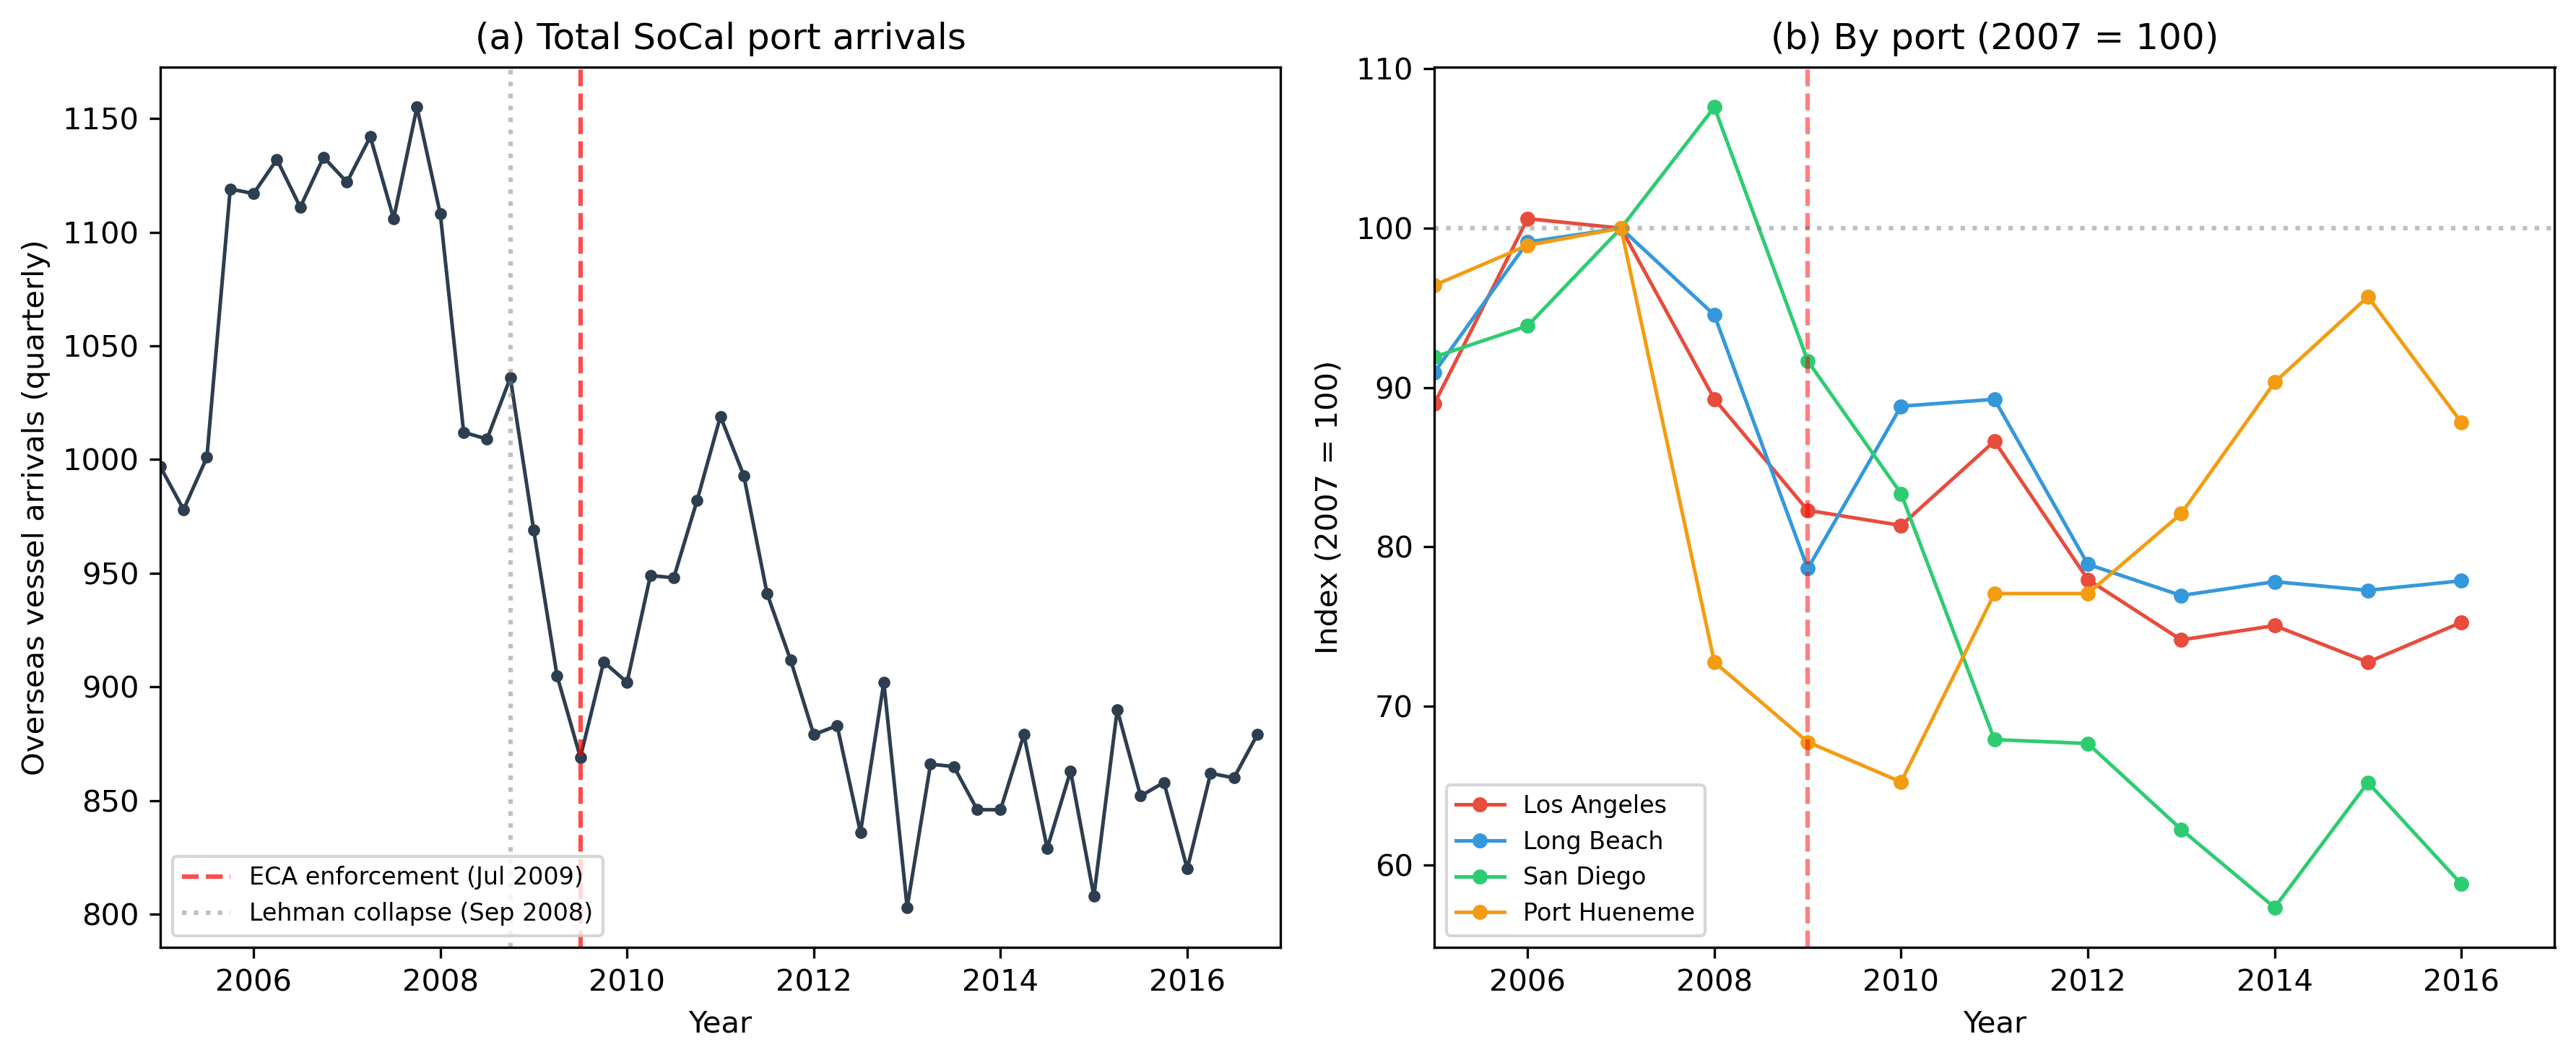
\includegraphics[width=0.95\textwidth]{../output/figures/nbic_port_activity.png}
    \caption{Overseas vessel arrivals at Southern California ports}
    \label{fig:nbic_port_activity}
    \vspace{0.15em}
    \begin{flushleft}
        \footnotesize Note: Panel~(a): total quarterly overseas vessel arrivals at four Southern California ports (Los Angeles, Long Beach, San Diego, Port Hueneme). Panel~(b): arrivals by port, indexed to 2007\,=\,100. Dashed red line marks ECA enforcement (July 2009); dotted gray line marks the Lehman collapse (September 2008). Data source: National Ballast Information Clearinghouse (NBIC).
    \end{flushleft}
\end{figure}

Figure~\ref{fig:crisis_decomposition} presents the core identification argument by juxtaposing port activity with the kelp event study. Panel~(a) shows the same data aggregated to annual frequency (2007\,=\,100). Port activity fell to approximately 81\% of its 2007 level in 2009 and never recovered: by the end of the sample, arrivals stood at only 76\% of the pre-crisis baseline. If reduced economic activity at ports---rather than the ECA---were driving kelp improvements, the effect should fade as ports remain depressed or should intensify as port activity declines further. Neither pattern is consistent with the event study in Panel~(b), which shows positive coefficients for the interaction of shipping exposure and post-2009 indicators despite the continued depression in port activity.

\begin{figure}[H]
    \centering
    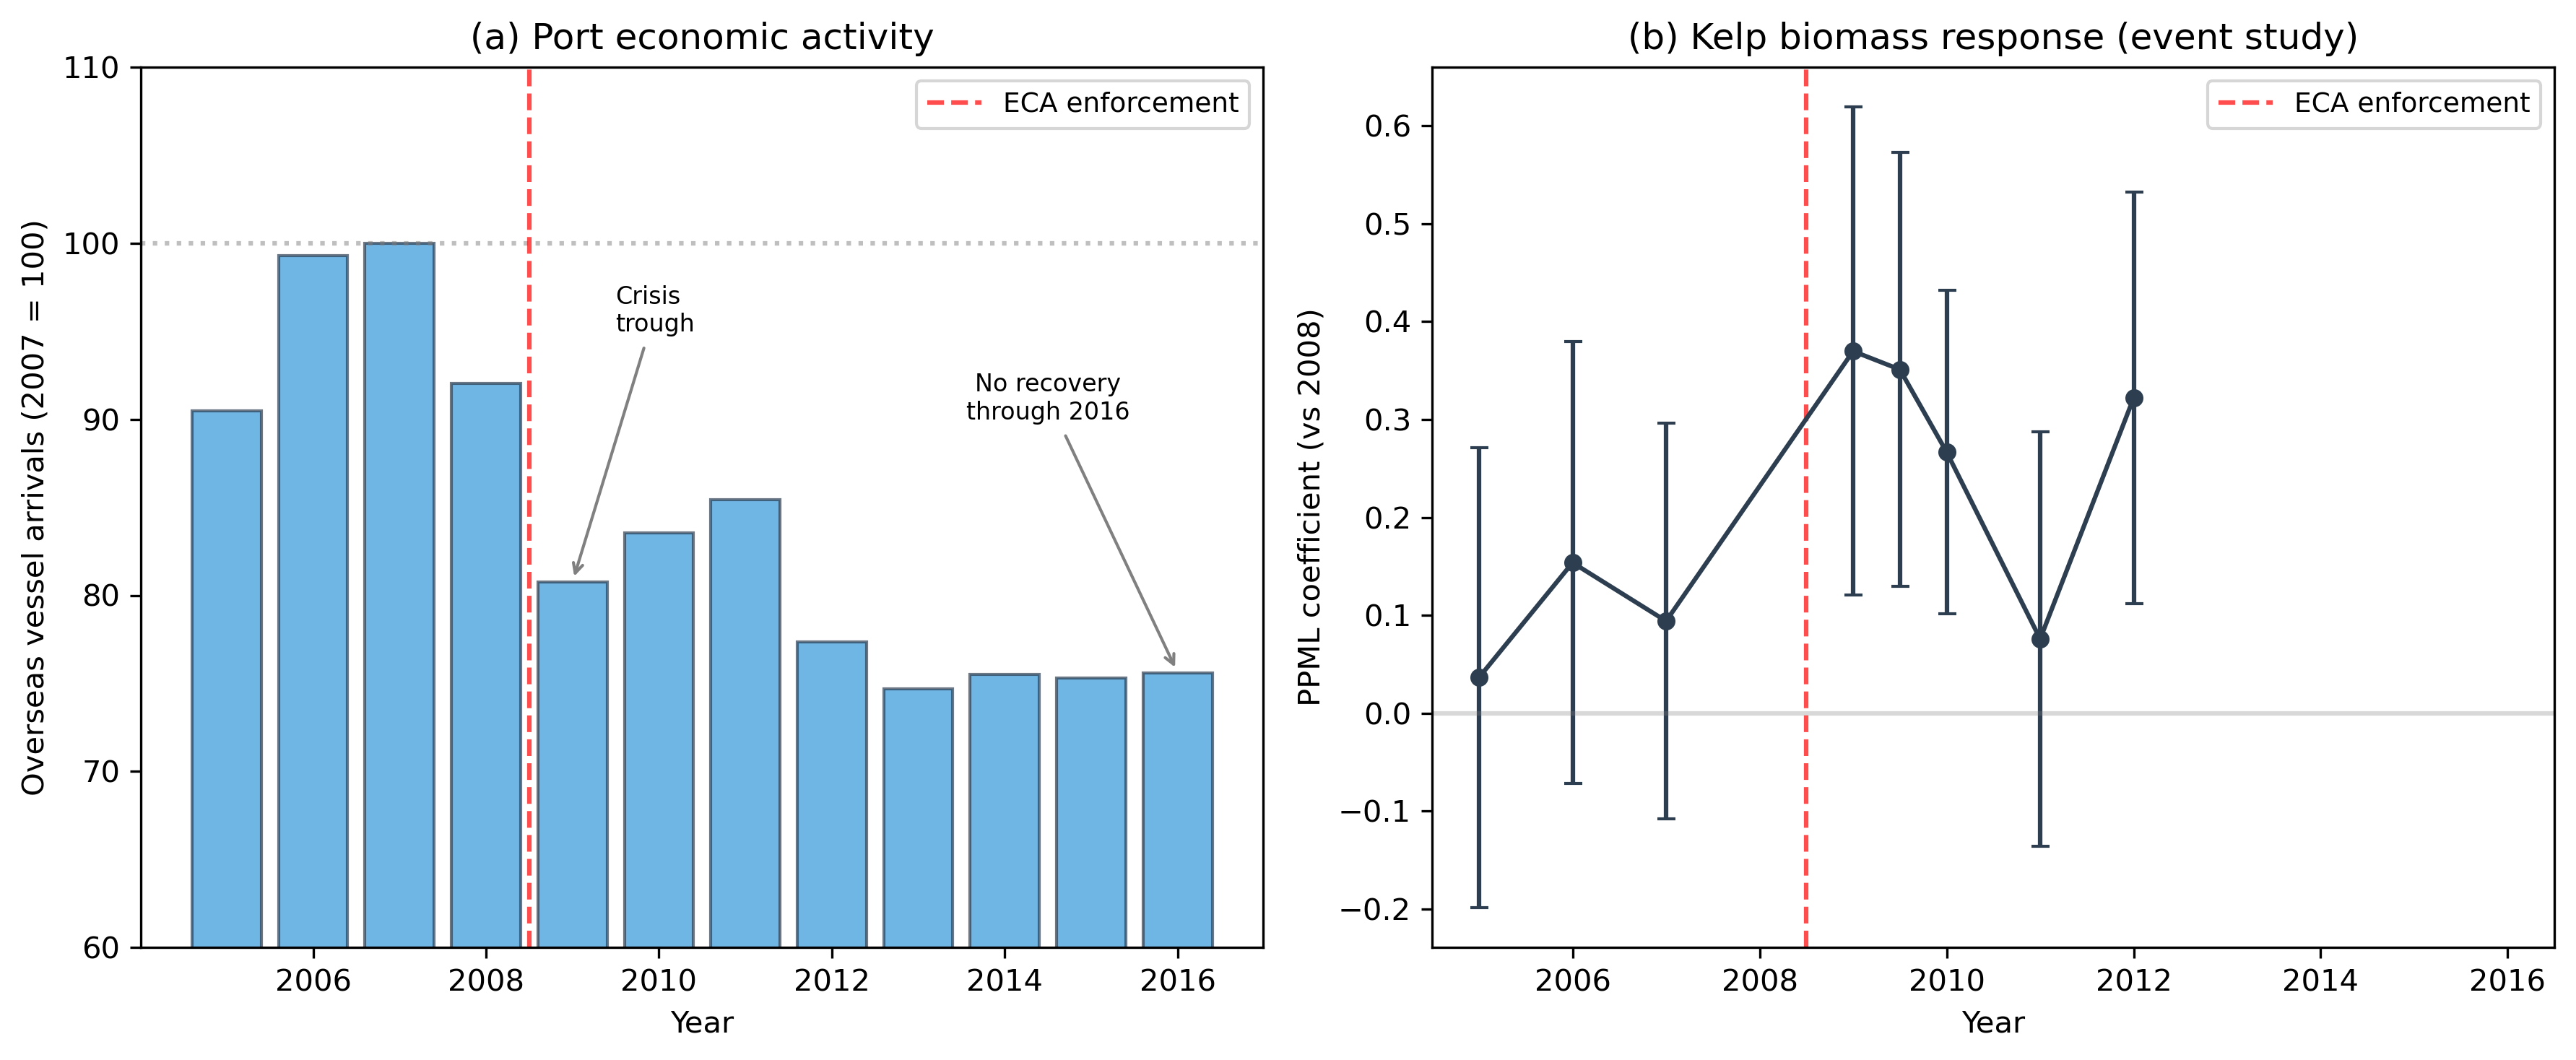
\includegraphics[width=0.95\textwidth]{../output/figures/crisis_decomposition.png}
    \caption{Port economic activity and kelp biomass response}
    \label{fig:crisis_decomposition}
    \vspace{0.15em}
    \begin{flushleft}
        \footnotesize Note: Panel~(a): annual overseas vessel arrivals at four Southern California ports (Los Angeles, Long Beach, San Diego, Port Hueneme), indexed to 2007\,=\,100. Data source: National Ballast Information Clearinghouse (NBIC). Panel~(b): PPML event-study coefficients from Eq.~(\ref{eq:es}), using vessel distance as treatment intensity (reference year: 2008). The dashed vertical line marks ECA enforcement (July 2009). 95\% confidence intervals based on standard errors clustered at the cell level.
    \end{flushleft}
\end{figure}

Table~\ref{tab:crisis_robustness} formalizes this argument by adding the log of distance-weighted port arrivals as a time-varying control in the PPML specification. Panel~A reproduces the baseline estimates from Table~\ref{tab:main_2009}. Panel~B adds the port-activity control. The shipping-exposure coefficient is virtually unchanged: the attenuation is at most 2\% across the four specifications, and all coefficients remain statistically significant at the 1\% level. The port-activity variable itself enters positively and significantly (coefficients between 0.58 and 0.68, $p<0.01$), indicating that it has genuine explanatory power for kelp outcomes---yet it does not absorb the treatment effect. This stability demonstrates that the differential kelp improvement in high-shipping cells is not driven by the differential reduction in port economic activity during the financial crisis.

\begin{table}[H]
  \centering
  \caption{Robustness to controlling for port economic activity}
  \label{tab:crisis_robustness}
  \def\sym#1{\ifmmode^{#1}\else\(^{#1}\)\fi}
\begin{tabular}{l*{4}{c}}
\hline\hline
                    &\multicolumn{2}{c}{Distance Traveled}&\multicolumn{2}{c}{Vessel Count}\\
                    \cmidrule(lr){2-3}\cmidrule(lr){4-5}
                    &\multicolumn{1}{c}{(1)}&\multicolumn{1}{c}{(2)}&\multicolumn{1}{c}{(3)}&\multicolumn{1}{c}{(4)}\\
                    &\multicolumn{1}{c}{Biomass}&\multicolumn{1}{c}{Area}&\multicolumn{1}{c}{Biomass}&\multicolumn{1}{c}{Area}\\
\hline
\multicolumn{5}{l}{\textit{Panel A: Baseline (no port activity control)}}\\[0.3em]
Post 2009 $\times$ Exposure&     0.1361\sym{***}&     0.1317\sym{***}&     0.1548\sym{***}&     0.1493\sym{***}\\
                    &             (0.0359)&             (0.0352)&             (0.0432)&             (0.0424)\\
[0.8em]
\multicolumn{5}{l}{\textit{Panel B: Controlling for port economic activity}}\\[0.3em]
Post 2009 $\times$ Exposure&     0.1363\sym{***}&     0.1319\sym{***}&     0.1520\sym{***}&     0.1465\sym{***}\\
                    &             (0.0360)&             (0.0353)&             (0.0434)&             (0.0426)\\
[0.3em]
Log port arrivals   &     0.6831\sym{***}&     0.6698\sym{***}&     0.5851\sym{***}&     0.5751\sym{***}\\
                    &             (0.2084)&             (0.2081)&             (0.2011)&             (0.2009)\\
[0.5em]
\hline
Observations        &      3880         &      3880         &      3880         &      3880         \\
Controls            &         Yes         &         Yes         &         Yes         &         Yes         \\
Cell FE             &         Yes         &         Yes         &         Yes         &         Yes         \\
Year-Quarter FE     &         Yes         &         Yes         &         Yes         &         Yes         \\
\hline\hline
\end{tabular}
  \vspace{0.5em}

  \begin{minipage}{\linewidth}
  \footnotesize
  \textit{Notes:} PPML estimates of Eq.~(\ref{eq:cdid}). Panel~A: baseline specification (identical to Table~\ref{tab:main_2009}). Panel~B: adds log distance-weighted overseas vessel arrivals at Southern California ports (NBIC data) as a time-varying control. The port-activity variable is constructed as the inverse-distance-weighted sum of quarterly arrivals across four ports (Los Angeles, Long Beach, San Diego, Port Hueneme) for each kelp hexagonal cell. All specifications include kelp-cell and year--quarter fixed effects. Sample: Southern California (32\textdegree--36\textdegree\,N), 2005--2016, restricted to cells with at least two vessel passages per month on average (81 clusters). Standard errors clustered at the cell level in parentheses.\\
  \sym{*} \(p<0.10\), \sym{**} \(p<0.05\), \sym{***} \(p<0.01\).
  \end{minipage}
\end{table}

The combination of these two findings---coefficient stability when controlling for port activity, and the divergent timing of port depression versus kelp improvement---provides evidence that the financial crisis does not confound the estimated ECA effect.

\newpage

\section{Anticipation and Treatment Timing}\label{appendix_anticipation}

A potential concern with our identification strategy is anticipation. The California Air Resources Board (CARB) adopted the ocean-going vessel fuel regulation in 2008, and vessel operators may have begun adjusting their routes before the July 2009 enforcement date. If such adjustments altered the \emph{spatial pattern} of shipping exposure, our treatment variable---measured during January--June 2009---could reflect anticipatory routing rather than the pre-policy equilibrium, biasing our estimates.

There are strong economic reasons to doubt that anticipation is empirically relevant in this setting. The regulation imposes the use of low-sulfur marine fuel within the ECA, which is substantially more expensive than the heavy fuel oil used outside it \citep{Klotz2022}. Switching to compliant fuel thus entails a direct marginal cost increase on every voyage entering the zone. Vessel operators therefore have a clear incentive to \emph{delay} compliance until enforcement begins, not to anticipate it: using low-sulfur fuel before it is required would raise operating costs with no offsetting regulatory benefit. Anticipation through \emph{route adjustments}---sailing outside the ECA to avoid the zone entirely---is equally unlikely before enforcement, since the penalty for noncompliance did not apply until July 2009. In short, the cost structure of the regulation creates a strong incentive to maintain pre-policy routing patterns until the enforcement date, making it improbable that the January--June 2009 treatment variable reflects anticipatory behavior. Nonetheless, to substantiate this reasoning empirically, we provide two formal tests below.

We cannot address this concern by constructing a pre-2009 treatment variable from AIS data, because global AIS coverage was limited before 2009 and the raw AIS files in our dataset begin in January 2009. Instead, we provide two pieces of evidence that anticipation did not distort the spatial distribution of shipping across kelp cells.

\paragraph{Temporal stability of cell-level shipping rankings.}
If anticipation had reshuffled the spatial pattern of vessel traffic during January--June 2009, we would expect that pattern to differ systematically from patterns observed in later years, when any anticipatory rerouting would have subsided. Figure~\ref{fig:temporal_stability} reports the Spearman rank correlation between the January--June 2009 measure and the corresponding full-year measure for 2009 through 2016, computed across the 81 cells in our estimation sample. For both vessel distance and vessel count, rank correlations are high ($\rho\geq 0.94$) in years unaffected by the boundary modification (2009, 2012--2014). The correlations drop in 2010--2011 ($\rho$ between 0.63 and 0.76), consistent with the 2011 boundary modification reshuffling traffic patterns in a subset of cells near the Channel Islands. Importantly, the correlations rebound sharply in 2012--2014 ($\rho\geq 0.94$), confirming that the long-run spatial ordering of cells by shipping intensity is highly persistent. The 2010--2011 dip does not threaten the 2009 identification---it reflects the 2011 policy shock, not anticipation of the 2009 rule---and the high correlations in all other years indicate that anticipatory rerouting did not meaningfully alter which cells were more or less exposed to vessel traffic.

\begin{figure}[H]
    \centering
    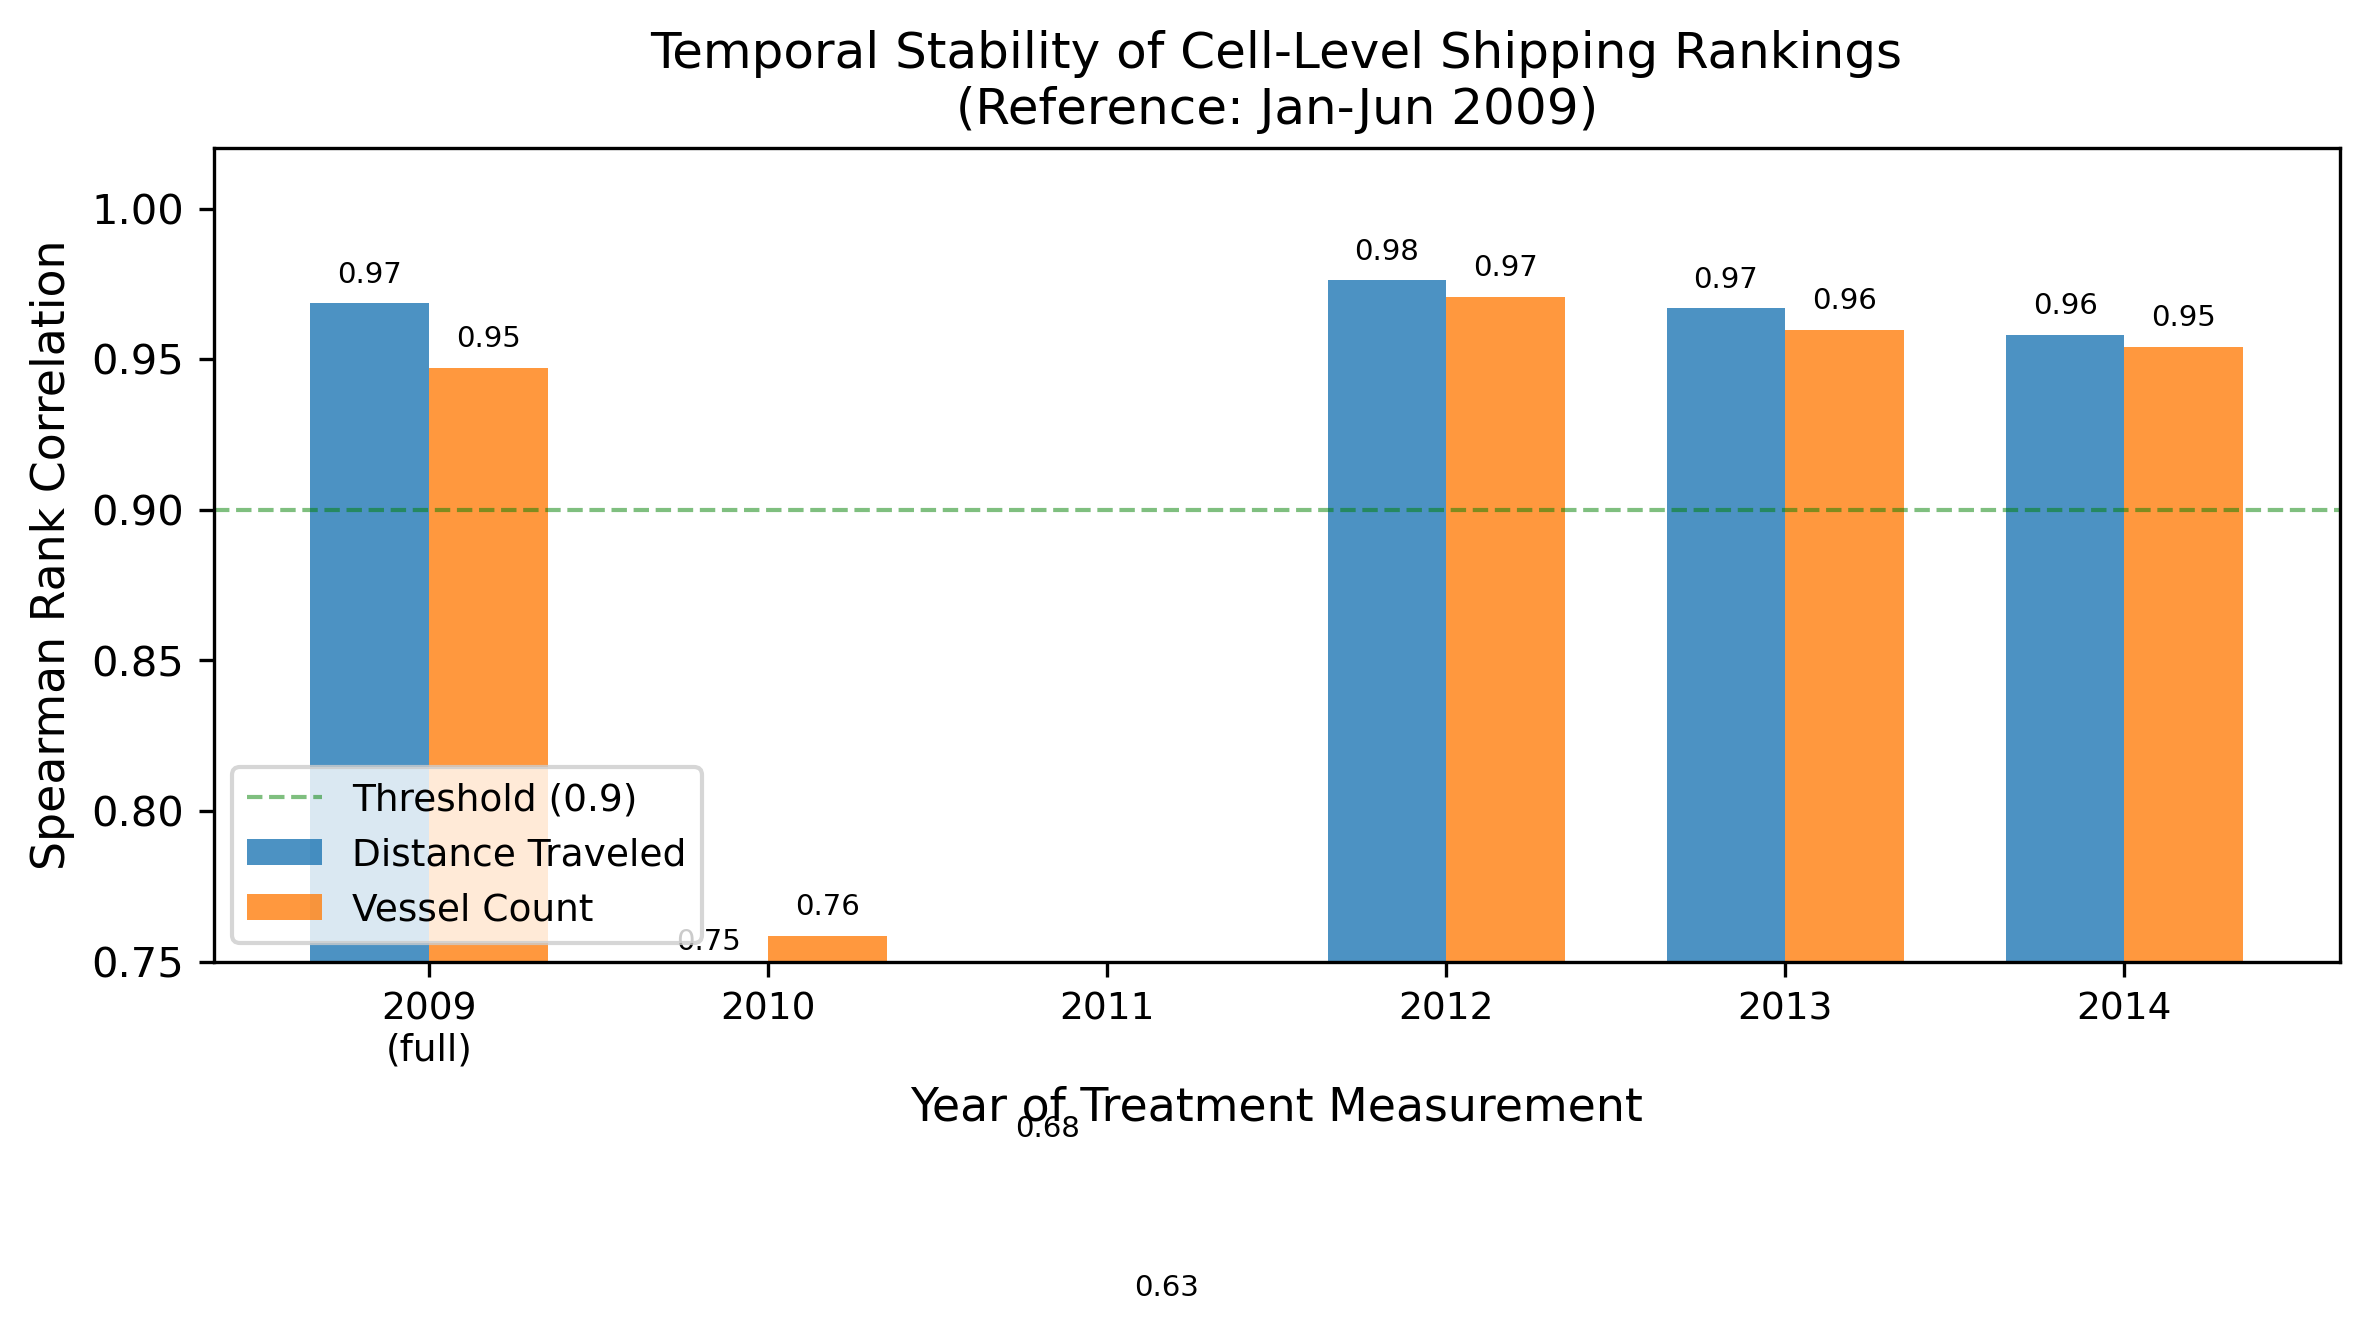
\includegraphics[width=0.7\textwidth]{../output/figures/temporal_stability_shipping.png}
    \caption{Temporal stability of cell-level shipping rankings}
    \label{fig:temporal_stability}
    \vspace{0.15em}
    \begin{flushleft}
        \footnotesize Note: Each bar reports the Spearman rank correlation between cell-level shipping exposure measured during January--June 2009 (the baseline treatment) and the corresponding full-year measure for the indicated year. Computed across the 81 cells in the estimation sample. The dashed line at 0.9 is shown for reference. Correlations are high ($\geq 0.94$) in all years except 2010--2011, where the boundary modification reshuffled traffic near the Channel Islands.
    \end{flushleft}
\end{figure}

\paragraph{Later-year treatments.}
As a stability check, we re-estimate Eq.~(\ref{eq:cdid}) replacing the January--June 2009 treatment with 2012 AIS data. Because the 2009 rule affected routing, the 2012 cross-section is not strictly predetermined; this exercise therefore tests whether the spatial pattern of the results is robust to using a post-policy proxy rather than providing an independent causal estimate. Table~\ref{tab:anticipation} reports the results. The coefficients are larger in magnitude than the baseline ($+0.156$ for distance, $+0.192$ for count), consistent with the spatial pattern of shipping becoming more precisely estimated as AIS coverage improves, and are all significant at the 1\% level. These results confirm that the choice of treatment timing does not qualitatively affect the main findings.

\begin{table}[H]
  \centering
  \caption{Anticipation robustness: Alternative treatment timing}
  \label{tab:anticipation}
  \def\sym#1{\ifmmode^{#1}\else\(^{#1}\)\fi}
\begin{tabular}{l*{4}{c}}
\hline\hline
                    &\multicolumn{2}{c}{Distance Traveled (km)}&\multicolumn{2}{c}{Vessel Count}\\
                    \cmidrule(lr){2-3}\cmidrule(lr){4-5}
                    &\multicolumn{1}{c}{(1)}&\multicolumn{1}{c}{(2)}&\multicolumn{1}{c}{(3)}&\multicolumn{1}{c}{(4)}\\
                    &\multicolumn{1}{c}{Biomass}&\multicolumn{1}{c}{Area}&\multicolumn{1}{c}{Biomass}&\multicolumn{1}{c}{Area}\\
\hline
\multicolumn{5}{l}{\textit{Panel A: Baseline (January--June 2009)}}\\[0.3em]
Post 2009 $\times$ Exposure&     0.1361\sym{***}&     0.1317\sym{***}&     0.1548\sym{***}&     0.1493\sym{***}\\
                    &             (0.0359)&             (0.0352)&             (0.0432)&             (0.0424)\\
[0.8em]
\multicolumn{5}{l}{\textit{Panel B: 2012 (post-adjustment)}}\\[0.3em]
Post 2009 $\times$ Exposure&     0.1559\sym{***}&     0.1512\sym{***}&     0.1922\sym{***}&     0.1860\sym{***}\\
                    &             (0.0389)&             (0.0382)&             (0.0489)&             (0.0481)\\
[0.5em]
\hline
Observations        &        3880         &        3880         &        3880         &        3880         \\
Controls            &         Yes         &         Yes         &         Yes         &         Yes         \\
Cell FE             &         Yes         &         Yes         &         Yes         &         Yes         \\
Year-Quarter FE     &         Yes         &         Yes         &         Yes         &         Yes         \\
\hline\hline
\end{tabular}

  \vspace{0.5em}
  \begin{minipage}{\linewidth}
  \footnotesize
  \textit{Notes:} PPML estimates of Eq.~(\ref{eq:cdid}). Each panel uses a different measurement period for the treatment variable: Panel~A uses January--June 2009 (baseline) and Panel~B uses full-year 2012 AIS data. Both panels use the same post-2009 indicator, controls (SST, precipitation, significant wave height), and cell and year--quarter fixed effects. Sample restricted to cells with at least two vessel passages per month on average. Standard errors clustered at the cell level in parentheses.\\
  \sym{*} \(p<0.10\), \sym{**} \(p<0.05\), \sym{***} \(p<0.01\).
  \end{minipage}
\end{table}

Taken together, the evidence indicates that the spatial distribution of shipping exposure across kelp cells was highly persistent throughout our study period. The January--June 2009 treatment variable is consistent with the long-run spatial pattern of maritime activity rather than transient anticipation-induced rerouting, and the main results are robust to alternative treatment timing.

\newpage

\section{Synthetic Differences-in-Differences}\label{appendix_sc}

A natural complement to the continuous DiD of Section~\ref{sec:empirical} would be a binary comparison of kelp outcomes in regulated California ports versus an unregulated port outside the boundary.\footnote{We estimated a standard two-way fixed-effects DiD comparing kelp cells near Los Angeles--Long Beach, San Diego, and Port Hueneme to cells near Ensenada, Mexico---a deep-water port embedded in the same Pacific shipping network but outside the California regulation. Post-2009 interaction terms were positive for all three treated ports; however, the standard errors from this specification are unreliable given the small number of clusters (see discussion in the text). These results are available on request.} However, because the regulation applies uniformly across California, the effective number of treatment clusters is very small (three treated port areas versus one control port). With only one control-group cluster, there is no within-group variation to estimate the control-group residual variance, making cluster-robust inference essentially impossible. Even wild bootstrap corrections become unreliable when the number of clusters falls below roughly five or six (\citealp{Cameron2008}; \citealp{Cameron2015}). This structural limitation, inherent in any single-jurisdiction policy, prevents credible inference from a binary design regardless of the number of sub-cluster observations within each port area.

The continuous DiD in Section~\ref{sec:empirical} partially addresses this concern by exploiting within-zone variation in exposure intensity, so that inference rests on 81 kelp-cell clusters rather than on a handful of port areas. The synthetic control exercise reported below provides a complementary external comparison that does not rely on within-California exposure variation: rather than selecting a single control port, it constructs a data-driven counterfactual from the full set of Mexican coastal hexagons using the method of \citet{Arkhangelsky2021}.

The analysis is conducted on a 10\,km hexagonal grid. We aggregate kelp biomass from 30\,m $\times$ 30\,m pixels to hexagons and construct an annual series for each hexagon. Treated units are coastal hexagons located within the 2009 regulated boundary; we exclude hexagons surrounding the ports already analyzed in the main text and those within the 2011 boundary modification area. The donor pool consists of coastal hexagons along the Mexican coast. Figure~\ref{fig:map_SC} displays the treated and donor units used in the synthetic control construction.

The synthetic control is constructed as a weighted combination of donor hexagons selected to replicate the treated pre-2009 biomass trajectory as closely as possible. The resulting weights are reported in Figure~\ref{fig:weights_SC}.

\begin{figure}[H]
    \centering
    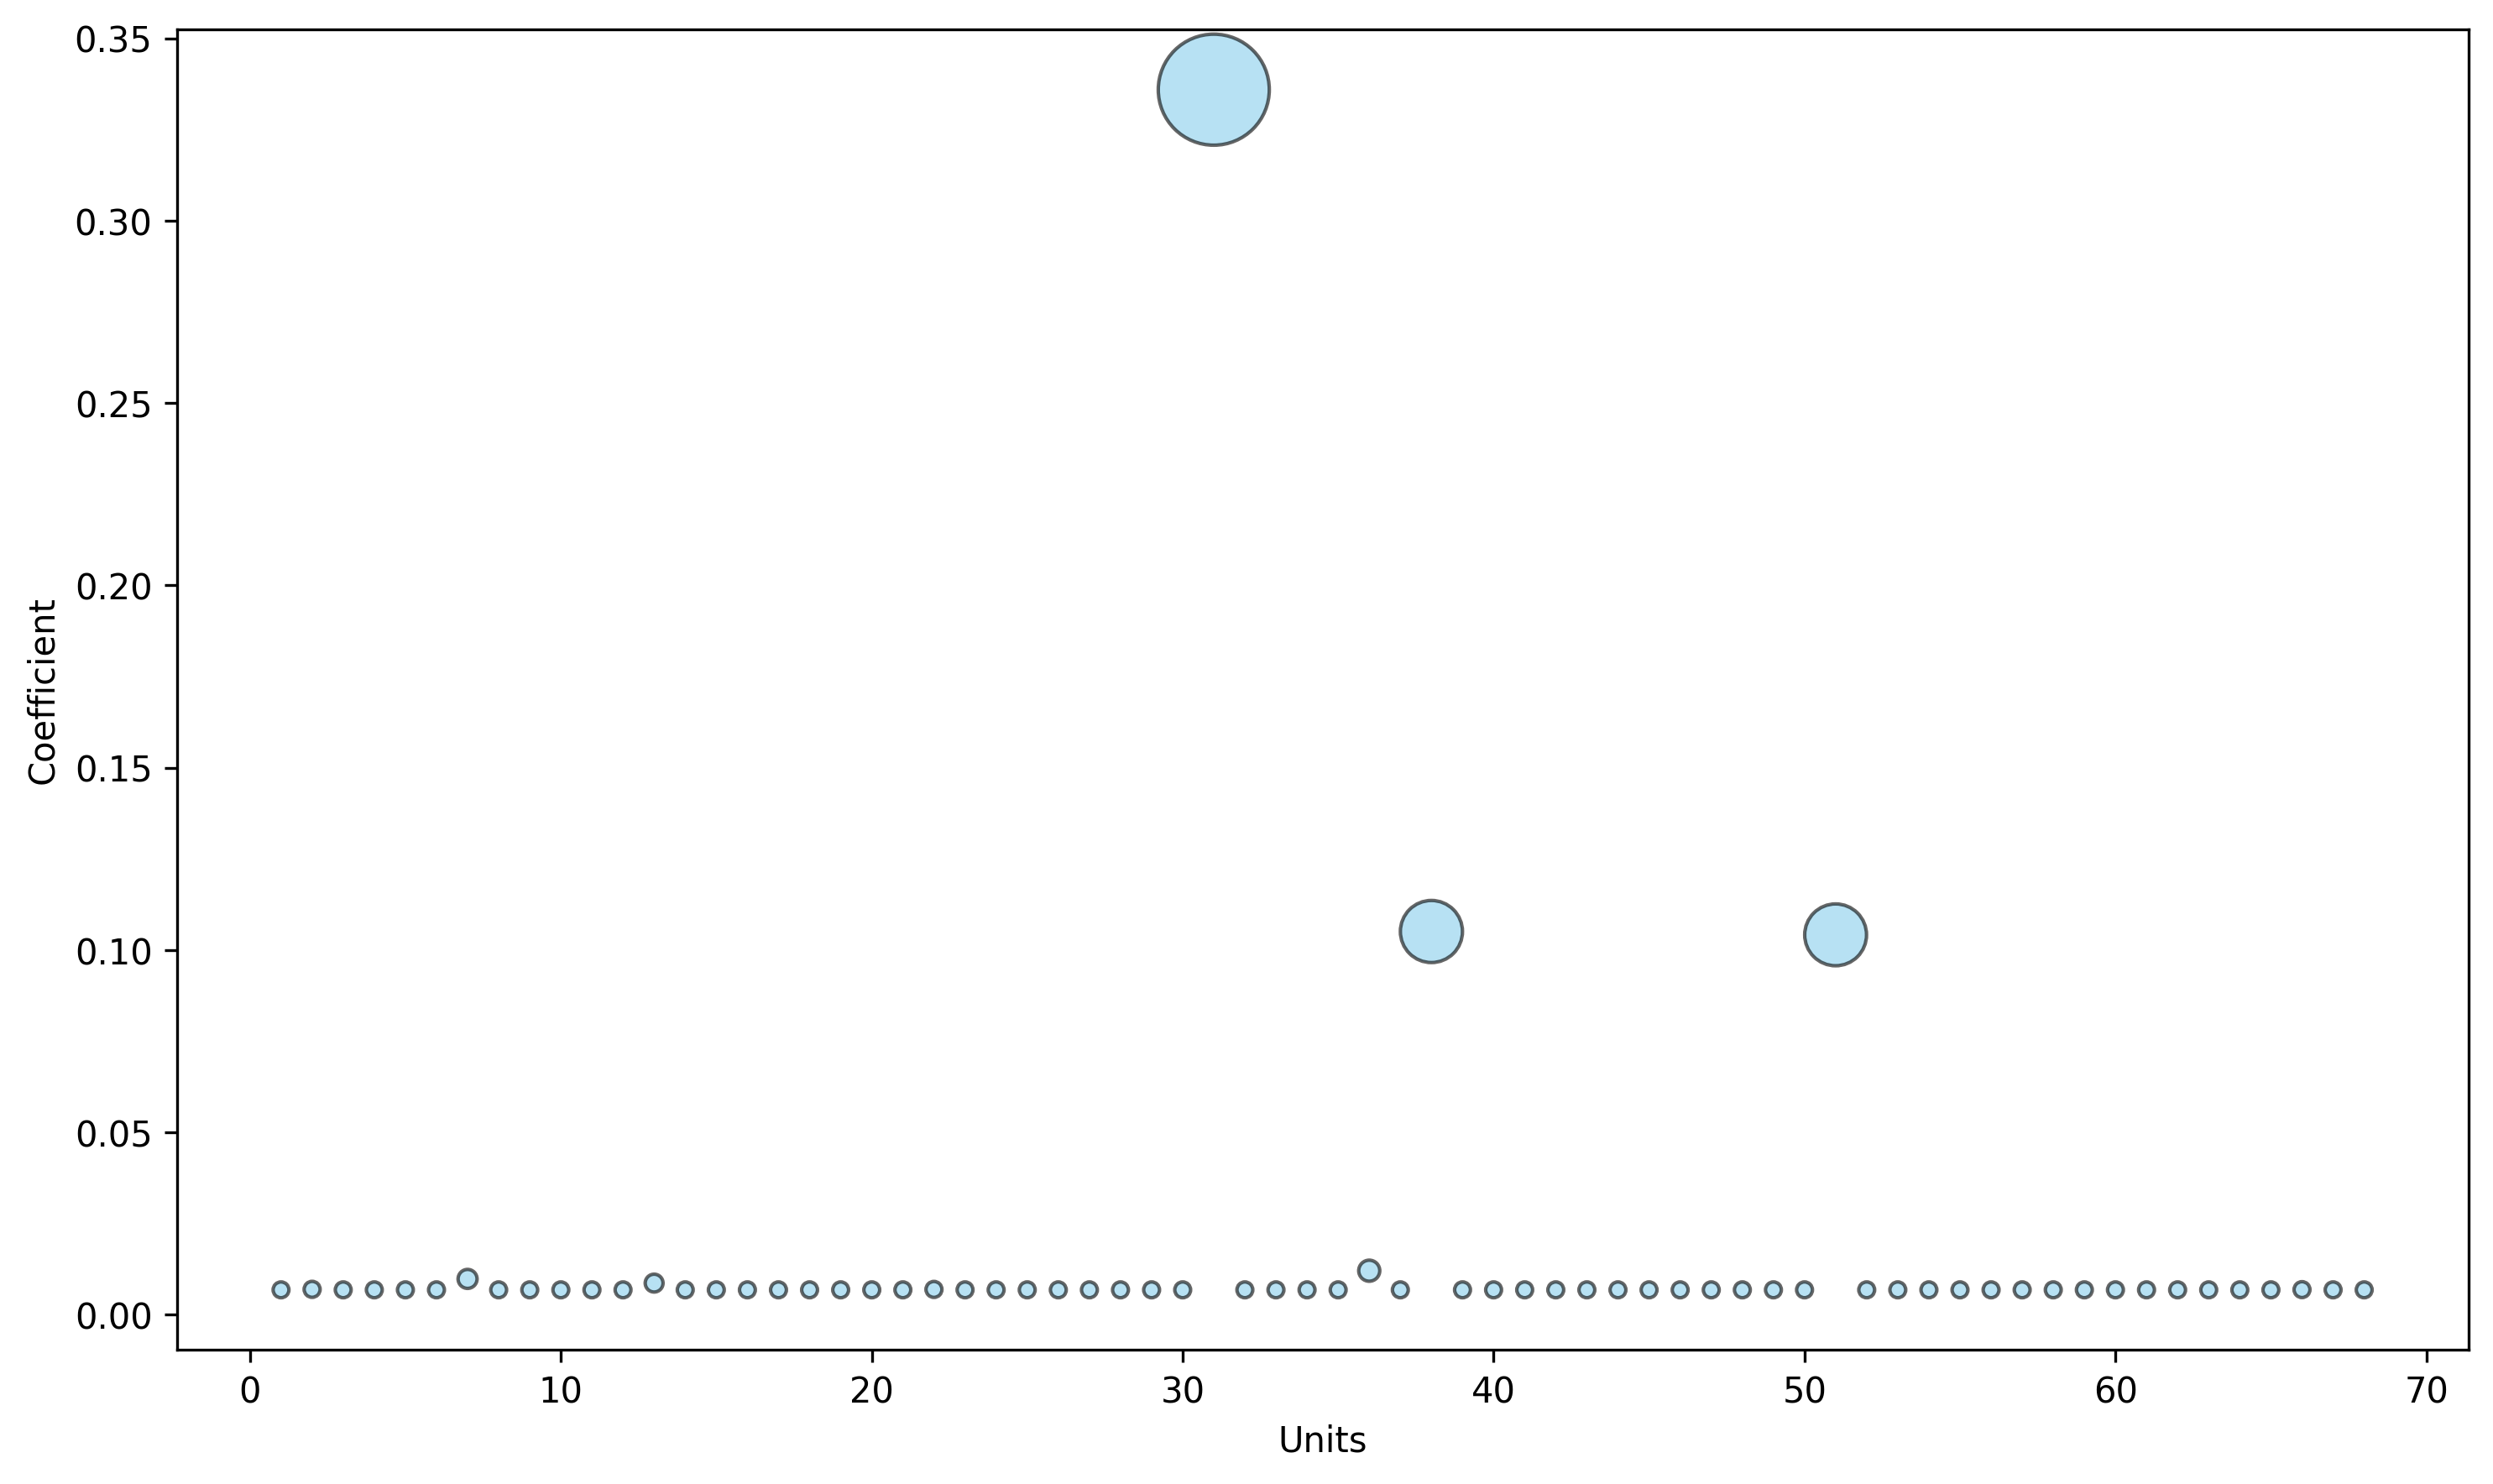
\includegraphics[width=0.6\textwidth]{../output/figures/weigth_sc.png}
    \caption{Synthetic control donor weights}
    \label{fig:weights_SC}
    \vspace{0.5em}
    \begin{flushleft}
{\footnotesize \textit{Notes:} Weights assigned to each donor hexagon in the synthetic control construction. Donor hexagons are Mexican coastal cells. Larger values indicate greater contribution to the synthetic counterfactual. The outcome variable used for matching is summed kelp biomass (kg) per hexagon-year.}
    \end{flushleft}
\end{figure}


A small number of donor hexagons receive most of the weight, which indicates that these locations are the most informative for matching the treated pre-period path. This feature is common in synthetic control applications.

\begin{figure}[H]
    \centering
    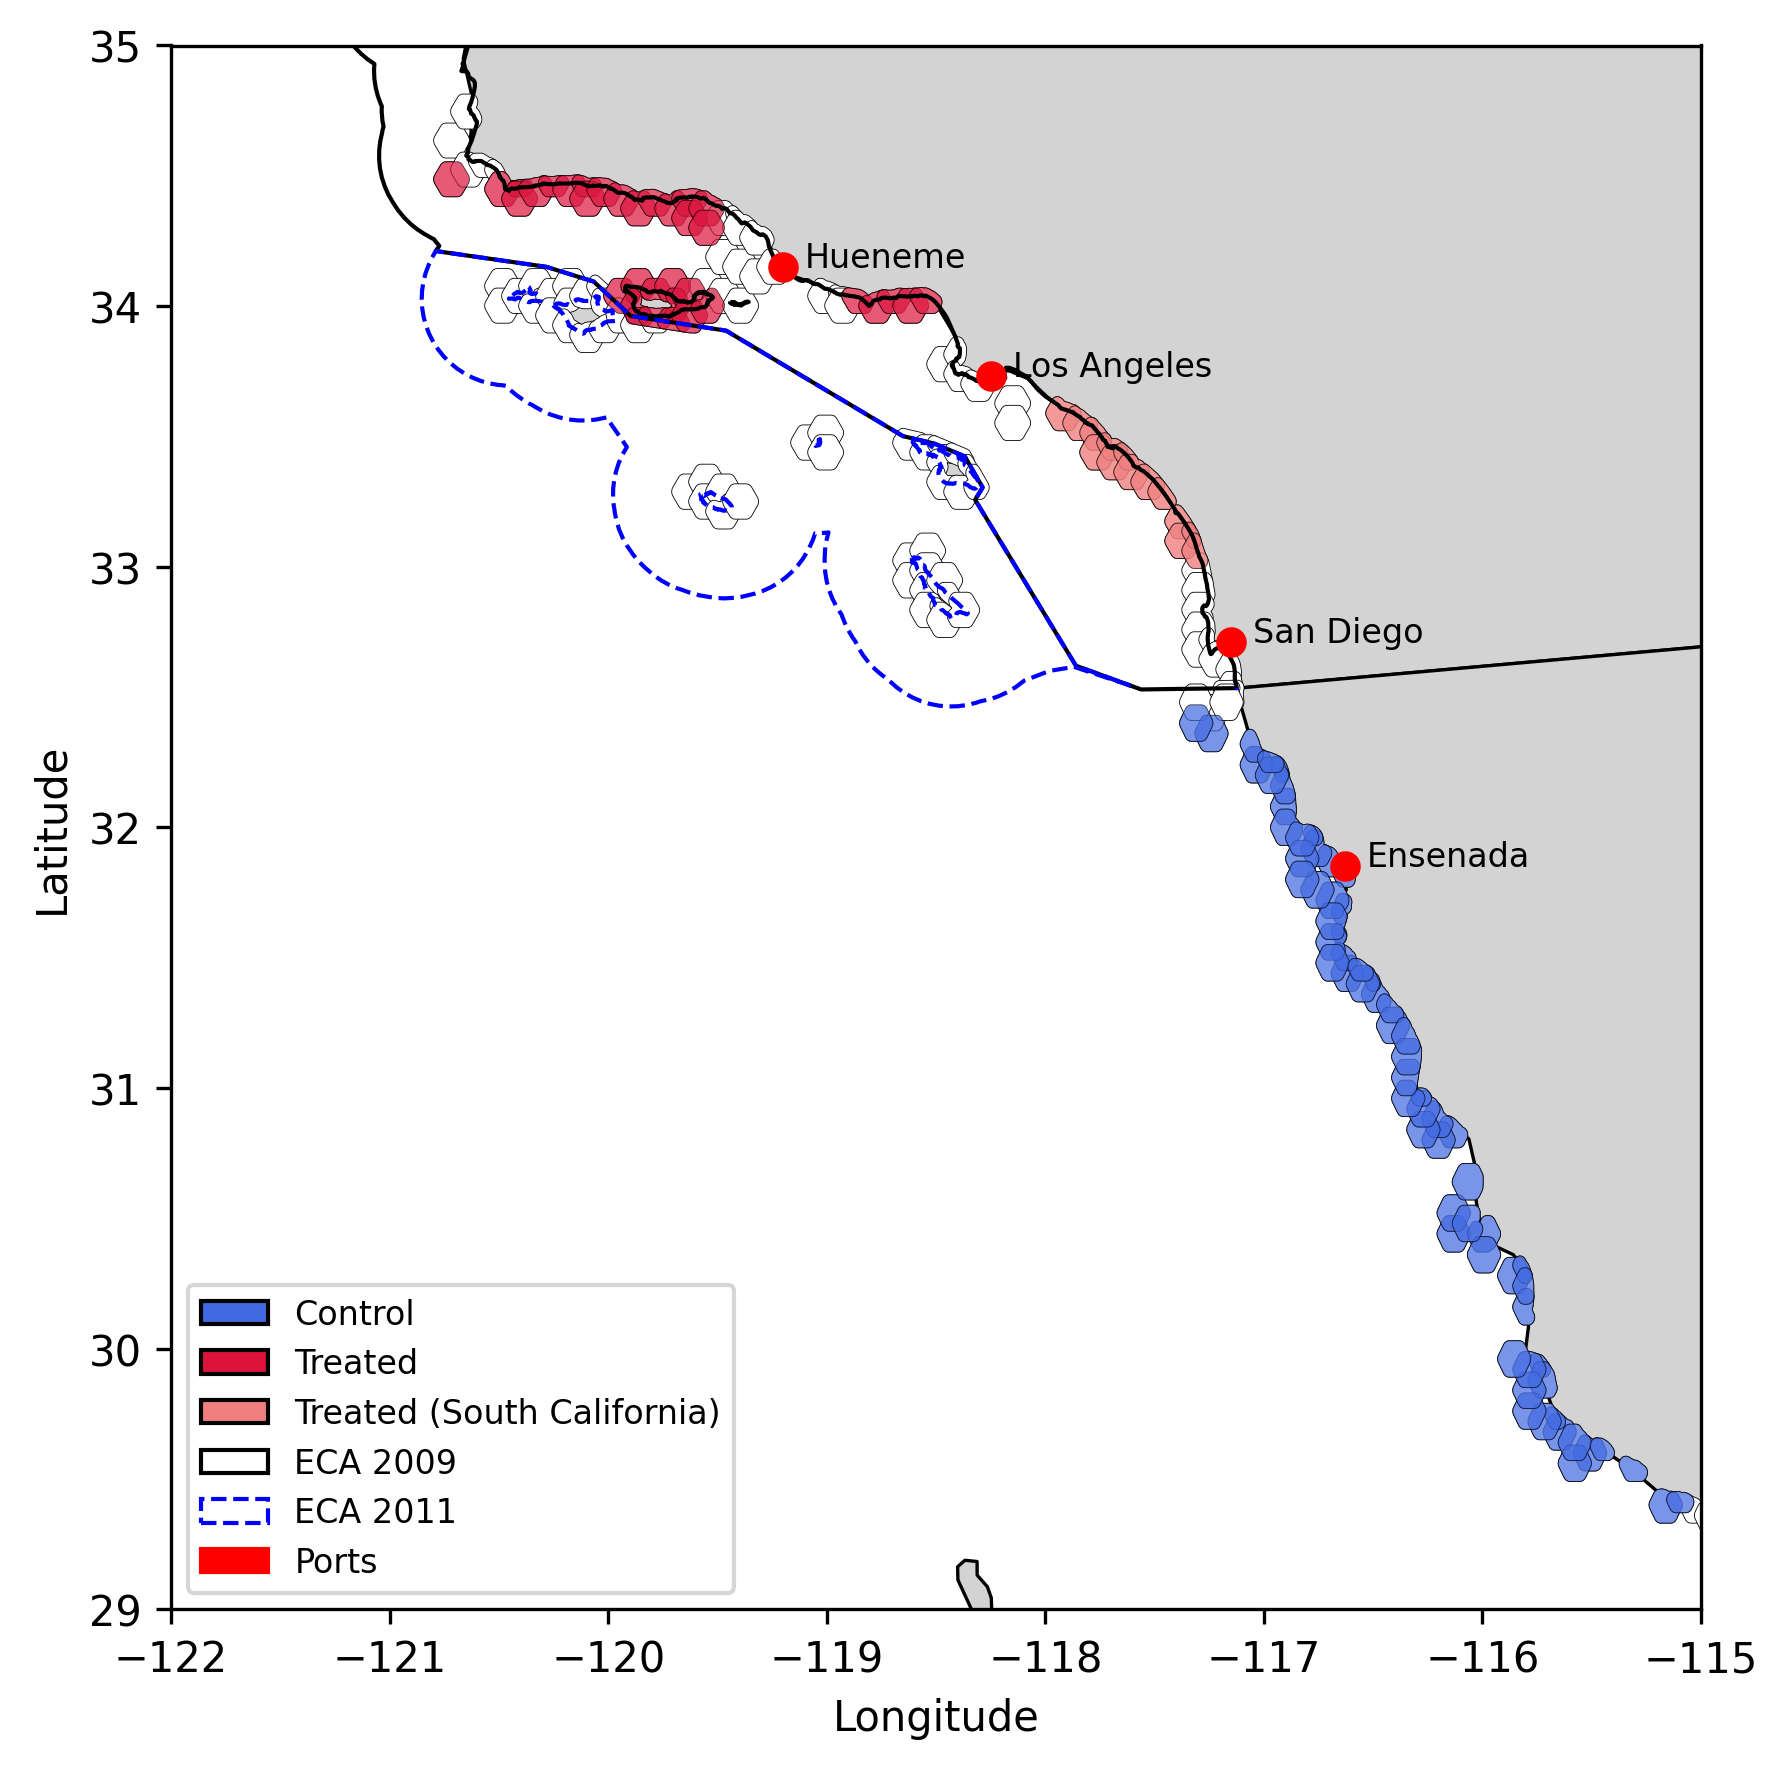
\includegraphics[width=0.7\textwidth]{../output/figures/map_SC.png}
    \caption{Map for the synthetic control analysis}
    \label{fig:map_SC}
    \vspace{0.5em}
    \begin{flushleft}
{\footnotesize \textit{Notes:} Red hexagons are treated units within the 2009 ECA boundary; light red hexagons are the southern California subset excluded in column~(2) of Table~\ref{tab:res_sc_ap}. Blue hexagons are the Mexican coastal donor pool. Geographic scope: Southern California to Baja California.}
    \end{flushleft}
\end{figure}

Table~\ref{tab:res_sc_ap} reports the estimated post-2009 effect for two treated samples: (1) all treated hexagons shown in red in Figure~\ref{fig:map_SC}, and (2) a treated sample excluding the southern California subset (light red in Figure~\ref{fig:map_SC}).


\begin{table}[H]
  \centering
  \caption{Synthetic differences-in-differences: Post-2009 ECA effect on kelp biomass}
  \label{tab:res_sc_ap}
  \begin{tabular}{l*{2}{c}}
\hline\hline
            &\multicolumn{1}{c}{(1)}&\multicolumn{1}{c}{(2)}\\
            &\multicolumn{1}{c}{All treated}&\multicolumn{1}{c}{Excl.\ Southern CA}\\
            &\multicolumn{2}{c}{Biomass (ln)}\\
\hline
Post 2009 (SDID)        &       1.391\sym{**}       &       1.911\sym{**} \\
                        &     (0.642)               &     (0.753)   \\
\hline
\(N\)                   &         819               &         721   \\
\hline\hline
\end{tabular}

  \vspace{0.5em}

  \begin{minipage}{\linewidth}
  \footnotesize
  \textit{Notes:} Synthetic differences-in-differences estimates \citep{Arkhangelsky2021} of the post-2009 ECA effect on log kelp biomass. The dependent variable is the natural log of summed kelp biomass (kg) per hexagon-year. Column~(1) uses all treated hexagons within the 2009 ECA boundary (red in Figure~\ref{fig:map_SC}); column~(2) excludes southern California hexagons (light red in Figure~\ref{fig:map_SC}). The donor pool consists of coastal hexagons along the Mexican coast. Standard errors in parentheses.\\
  \sym{*} \(p<0.10\), \sym{**} \(p<0.05\), \sym{***} \(p<0.01\).
  \end{minipage}
\end{table}


In both cases, the estimated effect is positive and statistically significant, indicating that biomass in treated California hexagons evolves more favorably after 2009 than in their synthetic counterparts constructed from the Mexican donor pool. Figure~\ref{fig:SC} shows the same result in levels: the synthetic series closely tracks the treated series prior to 2009 and then falls markedly afterwards, while the treated series remains comparatively stable. The post-2009 decline in the synthetic series reflects the realized evolution of the donor locations that best reproduce the treated pre-period trajectory.

\begin{figure}[H]
    \centering
    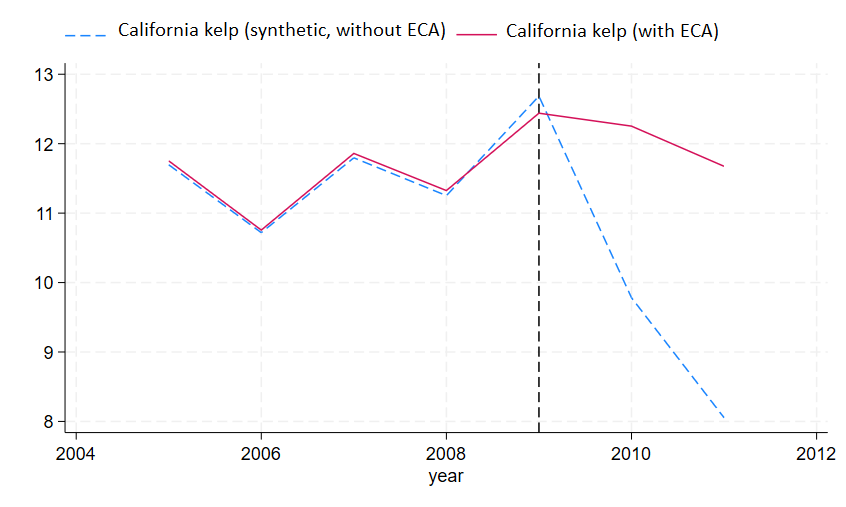
\includegraphics[width=0.8\textwidth]{../output/figures/SC.png}
    \caption{Synthetic control: treated vs.\ synthetic kelp biomass trends}
    \label{fig:SC}
    \vspace{0.5em}
    \begin{flushleft}
{\footnotesize \textit{Notes:} Annual kelp biomass (summed across hexagons) for treated cells within the 2009 ECA zone---excluding port areas analyzed in the main text---compared to a synthetic counterpart constructed from untreated Mexican coastal hexagons using the method of \citet{Arkhangelsky2021}. The vertical dashed line marks the 2009 ECA implementation.}
    \end{flushleft}
\end{figure}

\newpage

\section{After 2011 Boundary Modification}\label{appendix_after_2011}

Figure~\ref{fig:graph_exposure} plots the log of total distance traveled by vessels, averaged across hexagonal cells in each zone, comparing the 2009 regulated zone and the area corresponding to the 2011 boundary modification. The series illustrates a redistribution of traffic across these zones over time, consistent with route adjustments and the boundary modification documented in \citet{Klotz2022}.

\begin{figure}[H]
    \centering
    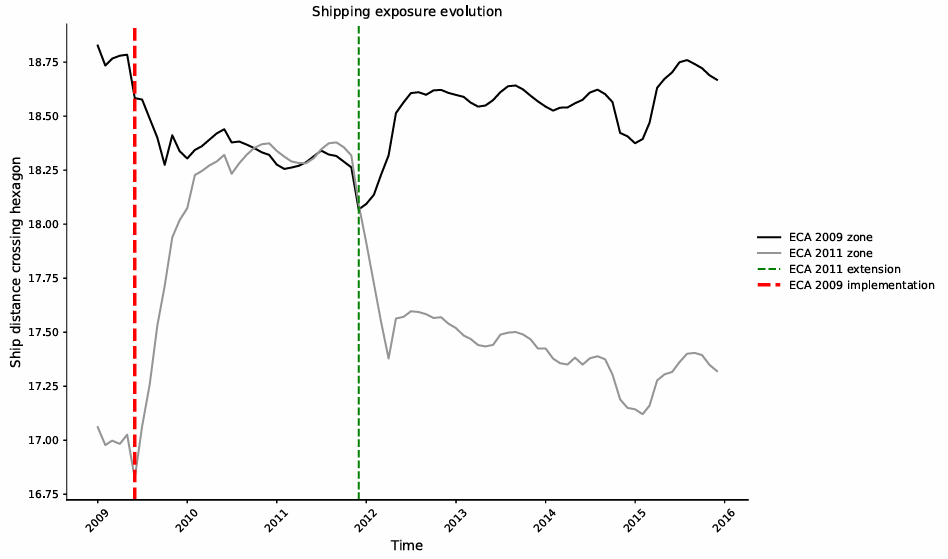
\includegraphics[width=0.9\textwidth]{../output/figures/shipping_exposure_png.png}
    \caption{Evolution of AIS shipping patterns}
    \label{fig:graph_exposure}
    \vspace{0.5em}
    \begin{flushleft}
{\footnotesize \textit{Notes:} Log of total distance traveled by vessels (km), averaged across hexagonal cells in each zone, for cells near kelp forests. ``ECA 2009 zone'' aggregates cells within the original 2009 regulated boundary; ``ECA 2011 zone'' aggregates cells in the 2011 boundary modification area. Data presented monthly from 2009 to 2016. Data source: AIS.}
    \end{flushleft}
\end{figure}

\newpage

\section{Robustness to Pre-Treatment Exposure: 2010 Shipping}\label{appendix_2010treat}

Because the 2011 boundary modification took effect in December 2011, the full-year 2011 treatment variable includes one month of post-modification routing. Although the main text argues that any contamination is quantitatively negligible and biased toward attenuation, we provide a direct robustness check by replacing the 2011 treatment with shipping exposure measured during 2010---a year entirely preceding the boundary change.

Table~\ref{tab:2010treat} reports PPML estimates that are otherwise identical to Table~\ref{tab:cdid2011}: same sample, same fixed effects, same controls. The only change is the treatment variable, which now uses logged vessel distance and count within a 20\,km buffer measured during 2010 instead of 2011.

\begin{table}[H]
  \centering
  \caption{Robustness: 2010 shipping exposure as treatment variable}
  \label{tab:2010treat}
  {
\def\sym#1{\ifmmode^{#1}\else\(^{#1}\)\fi}
\begin{tabular}{l*{4}{c}}
\hline\hline
                    &\multicolumn{2}{c}{Distance Traveled} &\multicolumn{2}{c}{Vessel Count}           \\\cmidrule(lr){2-3}\cmidrule(lr){4-5}
                    &\multicolumn{1}{c}{(1)}&\multicolumn{1}{c}{(2)}&\multicolumn{1}{c}{(3)}&\multicolumn{1}{c}{(4)}\\
                    &\multicolumn{1}{c}{Biomass}&\multicolumn{1}{c}{Area}&\multicolumn{1}{c}{Biomass}&\multicolumn{1}{c}{Area}\\
\hline
Post 2011 $\times$ Exposure (2010)&     -0.0766\sym{***}&     -0.0757\sym{***}&      -0.213\sym{***}&      -0.211\sym{***}\\
                    &    (0.0123)         &    (0.0122)         &    (0.0460)         &    (0.0451)         \\
[1em]
SST                 &      -7.046\sym{***}&      -6.950\sym{***}&      -7.118\sym{***}&      -7.022\sym{***}\\
                    &     (0.914)         &     (0.920)         &     (0.901)         &     (0.907)         \\
[1em]
Precipitation       &     -0.0480         &     -0.0505         &     -0.0452         &     -0.0478         \\
                    &    (0.0777)         &    (0.0771)         &    (0.0788)         &    (0.0781)         \\
[1em]
Significant Wave Height&      -3.326\sym{***}&      -3.245\sym{***}&      -3.363\sym{***}&      -3.282\sym{***}\\
                    &     (0.962)         &     (0.955)         &     (0.959)         &     (0.952)         \\
\hline
Cell FE             &         Yes         &         Yes         &         Yes         &         Yes         \\
Year-Quarter FE     &         Yes         &         Yes         &         Yes         &         Yes         \\
Observations        &        6000         &        6000         &        6000         &        6000         \\
\hline\hline
\end{tabular}
}

  \vspace{0.5em}

  \begin{minipage}{\linewidth}
  \footnotesize
  \textit{Notes:} PPML estimates of Eq.~(\ref{eq:cdid2011}) with shipping exposure measured during 2010 instead of 2011. The dependent variable is kelp biomass (kg) or canopy area (m$^{2}$). ``Distance Traveled (km)'' columns~(1)--(2) measure exposure by logged total distance traveled by vessels within a 20\,km buffer around each kelp hexagon during 2010; ``Vessel Count'' columns~(3)--(4) use the corresponding logged vessel count. All specifications include kelp-cell and year--quarter fixed effects. Standard errors clustered at the cell level in parentheses. Sample: Southern California (32\textdegree--36\textdegree\,N), 2005--2016.\\
  \sym{*} \(p<0.10\), \sym{**} \(p<0.05\), \sym{***} \(p<0.01\).
  \end{minipage}
\end{table}

All four coefficients are negative and statistically significant at the 1\% level. The vessel count coefficients are virtually unchanged ($-0.213$ with 2010 treatment versus $-0.210$ with 2011 treatment), well within each other's confidence intervals. The distance coefficients are smaller in absolute value ($-0.077$ versus $-0.093$), which is expected: the 2010 routing pattern predates the boundary modification by over a year, so it provides a slightly less precise spatial match to the corridors actually affected by the December 2011 change. The attenuation is consistent with classical measurement error in the treatment variable rather than with the 2011 results being inflated by post-modification contamination. In sum, using a purely pre-treatment measure of shipping exposure preserves the sign, significance, and economic interpretation of the main findings.

\newpage

\section{Treatment Correlation: 2009 vs.\ 2011 Exposure}\label{appendix_treat_corr}

The 2009 and 2011 specifications use different treatment variables measured at different dates: January--June 2009 AIS data for the main ECA analysis and full-year 2011 AIS data for the boundary modification. Because both variables capture the spatial distribution of vessel traffic around the same set of kelp cells, they are necessarily correlated. However, the strength and nature of this correlation matters for interpretation: if the two treatment variables were nearly collinear, the 2011 results would largely replicate the 2009 cross-sectional variation rather than exploiting independent spatial information from the boundary modification.

Figure~\ref{fig:treat_corr} plots the cell-level 2009 treatment against the 2011 treatment for both distance traveled and vessel count. The Pearson and Spearman correlations are reported in each panel. For vessel distance, the Pearson correlation is $r=0.67$ and the Spearman rank correlation is $\rho=0.69$; for vessel count, the correlations are lower at $r=0.58$ and $\rho=0.63$.

\begin{figure}[H]
    \centering
    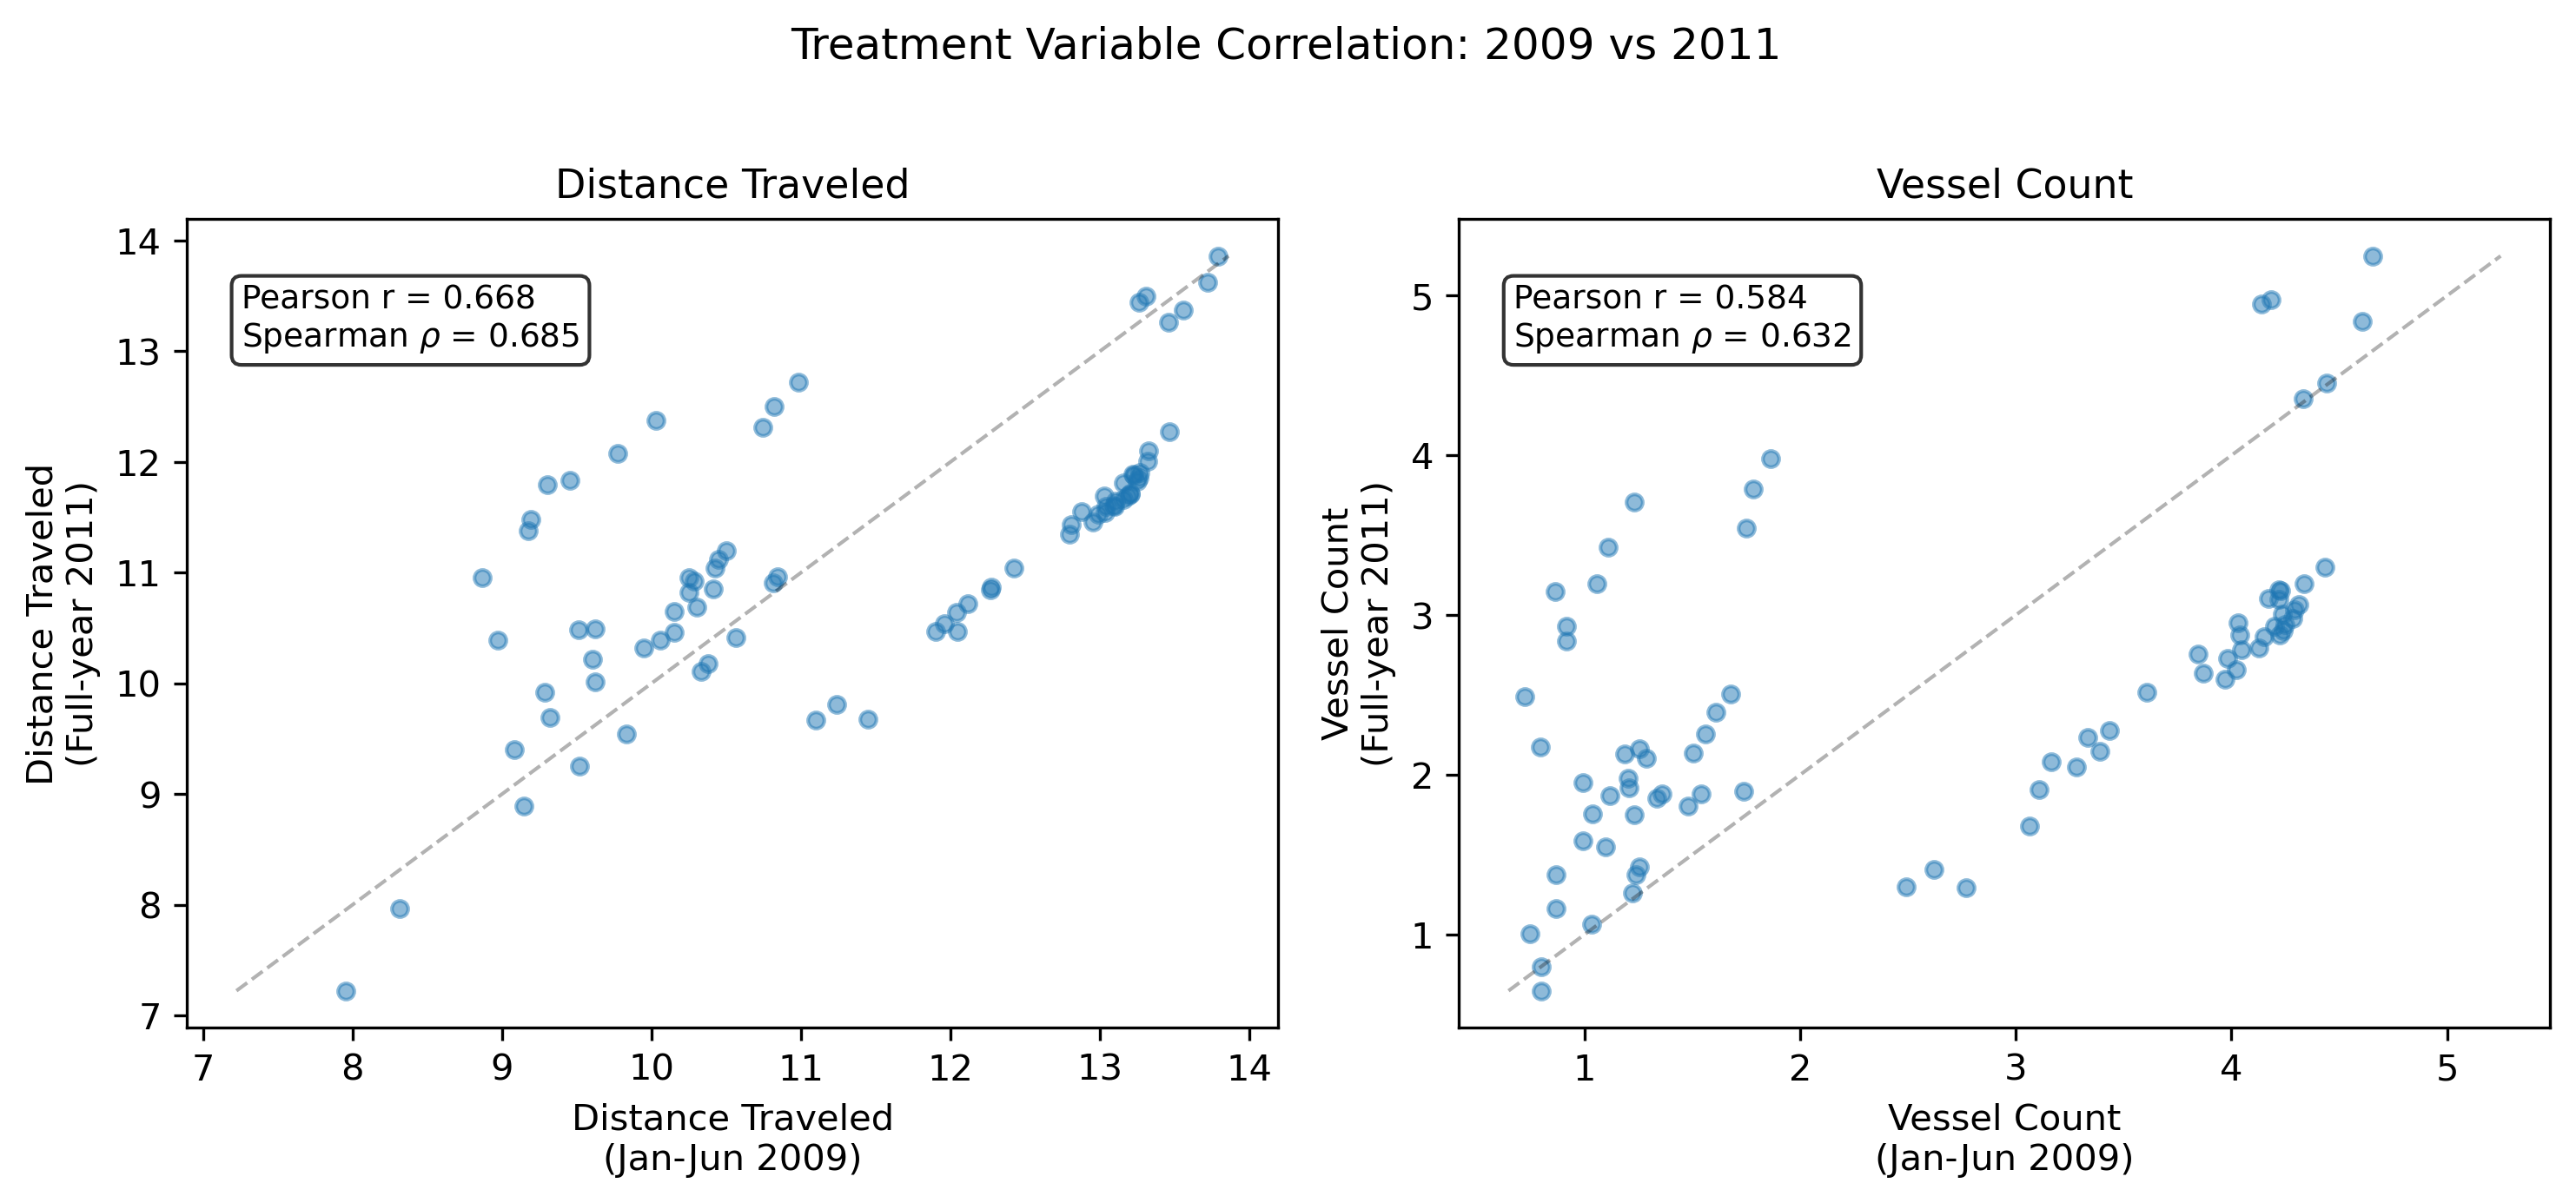
\includegraphics[width=0.85\textwidth]{../output/figures/treatment_correlation_2009_2011.png}
    \caption{Treatment variable correlation: 2009 vs.\ 2011 shipping exposure}
    \label{fig:treat_corr}
    \vspace{0.15em}
    \begin{flushleft}
        \footnotesize \textit{Notes:} Each point represents a kelp hexagonal cell. The $x$-axis measures log shipping exposure during January--June 2009 (the 2009 ECA treatment variable), and the $y$-axis measures log exposure during full-year 2011 (the boundary modification treatment variable). Left panel: log mean distance traveled (km) within a 20\,km buffer. Right panel: log mean vessel count. Both axes are in natural logs. Dashed line is the 45-degree reference. Pearson and Spearman correlations are reported in each panel.
    \end{flushleft}
\end{figure}

The correlations are moderate, indicating that the 2011 boundary modification genuinely reshuffled relative shipping intensities across cells. The scatter plots show clear dispersion around the 45-degree line, particularly for vessel count ($r=0.58$), where several cells that had moderate traffic in 2009 became heavily trafficked by 2011, and vice versa. This supports the argument that the two natural experiments exploit partially independent sources of spatial variation: the 2011 results are not mechanically driven by the same cross-sectional pattern as the 2009 specification, but instead reflect a distinct reallocation of traffic generated by the boundary modification.

\newpage

\section{Weighted PPML: 2011 Boundary Modification}\label{appendix_weighted_2011}

Table~\ref{tab:cdid2011} in the main text reports unweighted PPML estimates for the 2011 boundary modification. Table~\ref{tab:weighted_2011} below reports weighted estimates, where observations are weighted by log vessel count (20\,km buffer, 2011). The results are consistent in sign, significance, and magnitude: all four coefficients are negative and statistically significant at the 1\% level. The vessel traffic coefficient is $-0.102$ (weighted) versus $-0.093$ (unweighted); the vessel count coefficient is $-0.134$ (weighted) versus $-0.210$ (unweighted). The two sets of estimates fall within each other's confidence intervals, confirming that the 2011 results are insensitive to the weighting scheme.

\begin{table}[H]
  \centering
  \caption{Weighted PPML: Kelp outcomes and the 2011 boundary modification}
  \label{tab:weighted_2011}
  {
\def\sym#1{\ifmmode^{#1}\else\(^{#1}\)\fi}
\begin{tabular}{l*{4}{c}}
\hline\hline
                    &\multicolumn{2}{c}{Distance Traveled (km)} &\multicolumn{2}{c}{Vessel Count}           \\\cmidrule(lr){2-3}\cmidrule(lr){4-5}
                    &\multicolumn{1}{c}{(1)}&\multicolumn{1}{c}{(2)}&\multicolumn{1}{c}{(3)}&\multicolumn{1}{c}{(4)}\\
                    &\multicolumn{1}{c}{Biomass}&\multicolumn{1}{c}{Area}&\multicolumn{1}{c}{Biomass}&\multicolumn{1}{c}{Area}\\
\hline
Post 2011 $\times$ Exposure&      -0.102\sym{***}&      -0.101\sym{***}&      -0.134\sym{***}&      -0.133\sym{***}\\
                    &    (0.0251)         &    (0.0248)         &    (0.0473)         &    (0.0466)         \\
[1em]
SST                 &      -6.821\sym{***}&      -6.703\sym{***}&      -6.876\sym{***}&      -6.757\sym{***}\\
                    &     (1.003)         &     (1.004)         &     (1.002)         &     (1.003)         \\
[1em]
Precipitation       &      0.0432         &      0.0432         &      0.0430         &      0.0429         \\
                    &    (0.0824)         &    (0.0814)         &    (0.0820)         &    (0.0810)         \\
[1em]
Significant Wave Height&      -3.424\sym{***}&      -3.318\sym{***}&      -3.407\sym{***}&      -3.301\sym{***}\\
                    &     (0.978)         &     (0.973)         &     (0.978)         &     (0.973)         \\
\hline
Cell FE             &         Yes         &         Yes         &         Yes         &         Yes         \\
Year-Quarter FE     &         Yes         &         Yes         &         Yes         &         Yes         \\
Observations        &        5856         &        5856         &        5856         &        5856         \\
\hline\hline
\end{tabular}
}

  \vspace{0.5em}

  \begin{minipage}{\linewidth}
  \footnotesize
  \textit{Notes:} Weighted PPML estimates of Eq.~(\ref{eq:cdid2011}). The dependent variable is kelp biomass (kg) or canopy area (m$^{2}$). ``Distance Traveled (km)'' columns~(1)--(2) measure exposure by logged total distance traveled by vessels within a 20\,km buffer around each kelp hexagon during 2011; ``Vessel Count'' columns~(3)--(4) use the corresponding logged vessel count. Observations weighted by log vessel count (20\,km buffer, 2011). All specifications include kelp-cell and year--quarter fixed effects. Standard errors clustered at the cell level in parentheses. Sample: Southern California (32\textdegree--36\textdegree\,N), 2005--2016.\\
  \sym{*} \(p<0.10\), \sym{**} \(p<0.05\), \sym{***} \(p<0.01\).
  \end{minipage}
\end{table}

\end{document}




